\documentclass{article}

\usepackage[letterpaper, margin=1in]{geometry}
\usepackage{amsmath,amssymb}
\usepackage{enumerate}
\usepackage{booktabs}
\usepackage{graphicx}
\usepackage[amsmath,thmmarks,framed]{ntheorem}
\usepackage{authblk}
\usepackage{xcolor}
\definecolor{darkgreen}{rgb}{0.0,0.5,0.0}
\usepackage[colorlinks,linkcolor=red,citecolor=darkgreen,urlcolor=blue]{hyperref}
\hypersetup{
  pdftitle={Infinitely many primes p=m^2+n^2 with n<p^0.1129},
  pdfauthor={Xuda Ye}
}
\usepackage[numbers,square,comma,sort&compress]{natbib}

\newtheorem{theorem}{Theorem}
\newtheorem{lemma}{Lemma}
\newtheorem{corollary}[lemma]{Corollary}
\newtheorem{remark}[lemma]{Remark}
\newenvironment{proof}[1][Proof]{\par\medskip\noindent\textit{#1.}\ }{\hfill$\square$\par\medskip}

\newcommand{\Le}{\leqslant}
\newcommand{\Ge}{\geqslant}

\title{Infinitely Many Primes $p=m^2+n^2$ with $n<p^{0.1129}$}

\author{Xuda Ye}
\affil{Department of Mathematics, Purdue University, West Lafayette, IN 47907}
\date{\today}

\begin{document}
\maketitle

\begin{abstract}
We prove that infinitely many primes $p = m^2 + n^2$ have $n < p^{0.1129}$, and that infinitely many primes satisfy $\{\sqrt{p}\} < p^{-0.2742}$. This sharpens the exponents $0.119$ and $-0.262$ of Harman and Lewis (2001). Following their approach, we derive both statements from a lower bound of the correct order of magnitude for the number of Gaussian primes of norm between $X/2$ and $X$ in every sector of angle $X^{-0.3871}$, and we prove this bound with Harman's sieve and their arithmetic information. The new ingredients are three groupings of terms that their sieve discards: a factorization of a two-dimensional sum for the linear estimate, and two applications of the bilinear estimate to four-dimensional sums, one of them after a further application of Buchstab's identity. These groupings give the grouped terms asymptotic formulas, so that fewer terms are discarded. In addition, we give every step of the sieve argument in full, filling in the details that Harman and Lewis present briefly and making several of their statements and discarded regions precise, and we evaluate the losses of the discarded sums by two numerical methods.
\end{abstract}

\textbf{Keywords:} Gaussian primes, narrow sectors, Harman's sieve, Hecke characters, fractional part of $\sqrt{p}$.

\textbf{2020 MSC:} 11N36, 11N32, 11R44, 11J71.

\section{Introduction}
\label{sec: introduction}

A prime $p \equiv 1 \pmod 4$ is the norm $p = m^2 + n^2$ of a Gaussian prime $m + in$. Landau asked whether $n = 1$ occurs for infinitely many primes, that is, whether infinitely many primes have the form $m^2 + 1$ \citep{pintz2009landau}. The question is open. \citet{iwaniec1978almost} showed that infinitely many integers $m^2 + 1$ have at most $2$ prime factors. Primes $p = m^2 + n^2$ are known with $n$ in sparse sets of arithmetic form: the squares \citep{friedlander1998polynomial}, the squares of primes \citep{heathbrown2017prime}, and the integers $y^2 + 1$ \citep{merikoski2023polynomials}. These results restrict the form of $n$, not its size. A weaker form of Landau's question asks how small $n$ can be taken for infinitely many primes $p = m^2 + n^2$. With $m > n > 0$, the condition $n < p^{\theta}$ places the Gaussian prime $m + in$ inside a sector of angle about $p^{\theta - 1/2}$ next to the real axis. So the problem is one of Gaussian primes in narrow sectors.

Under the Riemann hypothesis for the Hecke $L$-functions of $\mathbb{Q}(i)$, \citet{ankeny1952representations} and \citet{kubilius1955problem} showed that infinitely many primes $p = m^2 + n^2$ have $n \ll \log p$. Without hypotheses, every sector of angle greater than $X^{-3/10 + \varepsilon}$, for fixed $\varepsilon > 0$, contains the expected number of Gaussian primes of norm in $(X, 2X]$, by a result of \citet{ricci1976local} quoted in \citet[\S1]{huang2020gaussian}. This covers $n < p^{\theta}$ for every $\theta > 1/5$. For smaller $\theta$, \citet{coleman1993rosser} obtained $n < p^{0.1631}$ with the Rosser--Iwaniec sieve in number fields. \citet{harman2001gaussian} used essentially the arithmetic information of Coleman with Harman's sieve \citep{harman2007prime}, and obtained $n < p^{0.119}$. Among the results that hold for every sector, this bound has remained the best known \citep[\S1.2]{jarviniemi2024gaussian}. \citet{harman2004prime} apply the same sieve to sectors in which the norm also lies in a short interval. Results that hold for almost all sectors go much further. \citet{huang2020gaussian} prove an asymptotic formula for the number of Gaussian primes of norm in $(X, 2X]$ in almost all sectors of angle greater than $X^{-3/5 + \varepsilon}$, for every fixed $\varepsilon > 0$. \citet{jarviniemi2024gaussian} find products of exactly $2$ Gaussian primes in almost all sectors of area $(\log X)^{15.1}$ in the disc of radius $X^{1/2}$.

If $p = m^2 + n^2$ with $n < p^{\theta}$, then
\begin{equation}
\label{eq: fractional part}
0 < \sqrt{p} - m = \frac{n^2}{\sqrt{p} + m} < p^{2\theta - 1/2}.
\end{equation}
Let $\{x\}$ denote the fractional part of $x$. Then $\{\sqrt{p}\} < p^{-(1/2 - 2\theta)}$ once $\theta < 1/4$. Harman and Lewis proved the bound $n < p^{\theta}$ with $\theta = 0.119$ \citep[Theorem~1]{harman2001gaussian}, and deduced $\{\sqrt{p}\} < p^{-0.262}$ for infinitely many primes as a corollary \citep[Theorem~4]{harman2001gaussian}. Earlier, \citet{balog1985distribution} and \citet{harman1983distribution} had obtained the exponent $1/4 - \varepsilon$ for every fixed $\varepsilon > 0$. The exponent $0.262$ has remained the best known \citep{li2025remark}. No exponent above $1/2$ is possible in such a bound, since $|\sqrt{p} - k| \Ge 1/(2\sqrt{p} + 1)$ for the integer $k$ nearest to $\sqrt{p}$.

Our main result is the following.

\begin{theorem}
\label{thm: primes}
There are infinitely many primes $p = m^2 + n^2$ with $m, n$ positive integers and $n < p^{0.1129}$. Consequently, there are infinitely many primes $p$ with $\{\sqrt{p}\} < p^{-0.2742}$.
\end{theorem}

Theorem~\ref{thm: primes} follows from a lower bound for the number of Gaussian primes in narrow sectors. Here and below, the Gaussian integers are the complex numbers $m + in$ with $m, n \in \mathbb{Z}$, which form the ring $\mathbb{Z}[i]$, and the norm of $m + in$ is $|m + in|^2 = m^2 + n^2$. The primes of $\mathbb{Z}[i]$ are the Gaussian primes. A non-zero Gaussian integer, and in particular a product of Gaussian integers, is identified with its associate of argument in $[0, \pi/2)$, and arguments are taken modulo $\pi/2$.

\begin{theorem}
\label{thm: sector}
Let $\theta = 0.1129$. There is a constant $c > 0$ such that, for every sufficiently large $X$,
\begin{equation}
\label{eq: sector bound}
\#\bigl\{ \varpi \in \mathbb{Z}[i] : \varpi \text{ Gaussian prime},\ X/2 \Le |\varpi|^2 < X,\ \psi \Le \arg \varpi < \psi + X^{\theta - 1/2} \bigr\} \Ge \frac{c X^{1/2 + \theta}}{\log X},
\end{equation}
which holds for every $\psi \in \mathbb{R}$.
\end{theorem}

The sector contains about $X^{1/2 + \theta}/(\pi \log X)$ Gaussian primes of norm in $[X/2, X)$ on average over $\psi$, so the lower bound \eqref{eq: sector bound} has the correct order of magnitude.

\begin{proof}[Proof of Theorem~\ref{thm: primes} from Theorem~\ref{thm: sector}]
Let $\theta = 0.1129$, and apply \eqref{eq: sector bound} with $\psi = 0$ and $X = 2^k$ for large $k$. The Gaussian primes of argument $0$ are the rational primes $\ell \equiv 3 \pmod 4$, and fewer than $X^{1/2}$ of them have norm $\ell^2 < X$. So the sector contains a Gaussian prime $\varpi = m + in$ with $m, n > 0$. Its norm $p = m^2 + n^2$ is a rational prime with $X/2 \Le p < X$. Since $\theta < 1/2$ and $p < X$,
\begin{equation*}
n = \sqrt{p}\, \sin(\arg \varpi) < \sqrt{p}\, X^{\theta - 1/2} < \sqrt{p}\, p^{\theta - 1/2} = p^{\theta}.
\end{equation*} The ranges $[X/2, X)$ for different $k$ are disjoint. So the primes $p$ are distinct for different $k$, and there are infinitely many of them. The bound $\{\sqrt{p}\} < p^{-0.2742}$ follows from \eqref{eq: fractional part}, because $1/2 - 2\theta = 0.2742$.
\end{proof}

\subsection{Outline of the method}
\label{subsec: method}

The proof of Theorem~\ref{thm: sector} refines the argument of \citet{harman2001gaussian}. Let $\mathcal{A}$ be the set of Gaussian integers in the sector of \eqref{eq: sector bound} with norm in $[X/2, X)$, and let $\mathcal{B}$ be the set of all Gaussian integers of the quadrant with norm in $[X/2, X)$, so $\mathcal{A} \subset \mathcal{B}$. The number of Gaussian primes in $\mathcal{A}$ is the number of elements of $\mathcal{A}$ without prime factors of norm below $X^{1/2}$. Buchstab's identity \eqref{eq: buchstab} decomposes this count into sums of two kinds. Sums of the first kind have an asymptotic formula: they equal $2X^{\theta - 1/2}/\pi$ times the corresponding sums for $\mathcal{B}$, up to a negligible error. Harman and Lewis derive these formulas from bounds for Hecke $L$-functions, through linear (Type~I) and bilinear (Type~II) estimates. A sum has such a formula when its primes can be combined into variables whose norms lie in the ranges that these estimates admit.

Sums of the second kind consist of non-negative terms that enter with the sign $+$, so a lower bound may omit them. They are discarded. Each discarded sum, taken over $\mathcal{B}$ and divided by the number of Gaussian primes in $\mathcal{B}$, tends to an integral \eqref{eq: loss} of Buchstab's function $\omega$ over a region of exponents. This integral is the loss of the sum, and the sum of the losses is the total loss $\Phi(\theta)$. The same decomposition holds for the number of Gaussian primes in $\mathcal{B}$. So, up to a negligible error, the number of Gaussian primes in $\mathcal{A}$ is at least $2X^{\theta - 1/2}/\pi$ times the difference between the number of Gaussian primes in $\mathcal{B}$ and the discarded sums over $\mathcal{B}$. With the losses of these sums, this gives the lower bound
\begin{equation}
\label{eq: lower bound intro}
\#\{\varpi \in \mathcal{A} : \varpi \text{ Gaussian prime}\} \Ge \frac{2X^{\theta - 1/2}}{\pi}\, \#\{\varpi \in \mathcal{B} : \varpi \text{ Gaussian prime}\}\, \bigl(1 - \Phi(\theta) - o(1)\bigr).
\end{equation}
So \eqref{eq: sector bound} holds, with $\theta$ in place of $0.1129$, for every $\theta \in (1/9, 1/8)$ with $\Phi(\theta) < 1$. For their decomposition, Harman and Lewis state that the total loss at $\theta = 0.119$ is below $0.943$ \citep[p.~134]{harman2001gaussian}.

Besides the prime number theorem in progressions modulo $4$, only the arithmetic information is quoted without proof. It consists of the sector inequality, the mean-value estimate for Hecke characters, the prime number theorem with Hecke characters, and Lemmas~6 and~7 of Harman and Lewis. Lemmas~\ref{lem: sector inequality} to~\ref{lem: type I input} of Appendix~\ref{app: arithmetic} state them.

\subsection{Contributions}
\label{subsec: contributions}

We add three groupings of terms that Harman and Lewis discard. A grouping combines the primes of a sum into the variables of the linear or bilinear estimate, after a further application of Buchstab's identity \eqref{eq: buchstab} where needed, and so gives an asymptotic formula to a set of terms on which their decomposition has none.
\begin{itemize}
\setlength{\itemsep}{0pt}
\item \emph{A new factorization on a region $\mathsf{R}$.} On a two-dimensional region $\mathsf{R}$ of terms $pq$, with $p$ and $q$ Gaussian primes, Harman and Lewis discard the whole sum. We apply Buchstab's identity, which introduces a third prime $r$, and then the linear estimate to the factorization $p \cdot (qr)$. Harman and Lewis apply the linear estimate after Buchstab's identity only to the factorization $(pq) \cdot r$. On $\mathsf{R}$ the product $pq$ is too large for the linear estimate, while $p$ and $qr$ satisfy its conditions, because $q$ is small.
\item \emph{The bilinear estimate with any set of primes on a region $\mathsf{G}$.} The other two groupings act on terms $pqrst$ in which two applications of Buchstab's identity have introduced primes $r$ and $s$, and $t$ is the remaining factor, the cofactor. Harman and Lewis discard these terms over four-dimensional regions, except on a few subregions. The bilinear estimate needs a prime variable and further variables $u$ and $v$ of norm at least about $X^{1/2 - \theta}$, and it applies at every level of sifting of $t$. On a region $\mathsf{G}$, we apply it with $s$ as the prime variable and with the product of a non-empty subset of $\{p, q, r\}$ as $u$. Harman and Lewis use the subset $\{p, r\}$, in one of their regions only.
\item \emph{A further Buchstab step on a region $\mathsf{L}$.} On a region $\mathsf{L}$, we apply Buchstab's identity once more, at a level below every fixed power of $X$, which introduces a prime $s'$ with $|s'| \Le |s|$. The linear estimate for $pqrs$ then treats the sum sifted at this level, and the bilinear estimate with $s'$ as its prime variable treats the sum over $s'$. Here $u$ may contain $s$, which on $\mathsf{G}$ is the prime variable.
\end{itemize}
Section~\ref{sec: outline} defines $\mathsf{R}$, $\mathsf{G}$ and $\mathsf{L}$ and places them in the decomposition.

Table~\ref{tab: roots} shows the effect of each grouping. With the regions derived from the lemmas of Section~\ref{sec: two primes} (Remark~\ref{rem: misprints}), the decomposition of Harman and Lewis has total loss $1$ at $\theta = 0.1167825$. This is just below the range from $0.117$ to $0.118$ in which, by \citet[p.~134]{harman2001gaussian}, the constant in their lower bound ceases to be positive. They add that they did not spend much time on the numerical calculations. Adding $\mathsf{R}$ moves the value $0.1167825$ to $0.1141073$, and adding $\mathsf{G}$ and $\mathsf{L}$ moves it to $0.1128554$, so that the total loss is below $1$ at $\theta = 0.1129$. The losses are computed in floating point by two methods (Section~\ref{sec: numerics}). At $\theta = 0.1129$ the total loss is $0.9990033$. The gap $1 - \Phi(0.1129) = 9.97 \times 10^{-4}$ is more than $800$ times each of the following: the difference between the totals of the methods, the error estimate of the second method, and the change of the total of the first method under refinement of its quadrature.

We also give in full several steps that \citet{harman2001gaussian} present briefly: the fundamental lemma invoked in their Lemmas~8, 9, 11 and~12, the proofs of their Lemmas~8 to~10, the removal of the conditions that couple the variables of their bilinear estimate, and the extension of their Lemma~14 that part~6 of their \S5 uses. Lemma~\ref{lem: fundamental}, Lemmas~\ref{lem: level large} and~\ref{lem: level small} with Corollary~\ref{cor: level one}, Lemma~\ref{lem: decoupling} and Lemma~\ref{lem: lemma 14} fill in these steps. Appendix~\ref{app: comparison} compares the two arguments item by item, including several statements and discarded regions that are made precise here.

\subsection{Structure of the paper}
\label{subsec: structure}

Section~\ref{sec: notation} fixes the notation. Section~\ref{sec: outline} states the decomposition: identity \eqref{eq: identity 37}, the ranges of Table~\ref{tab: ranges}, the groupings $\mathsf{R}$, $\mathsf{G}$ and $\mathsf{L}$, and the total loss \eqref{eq: total loss}. Section~\ref{sec: estimates} states the linear and bilinear estimates, a fundamental lemma over $\mathbb{Z}[i]$, and asymptotic formulas for sifting functions with a variable level, and Section~\ref{sec: decoupling} removes the conditions that couple the variables of a sum. Section~\ref{sec: two primes} treats the sums over two primes. Section~\ref{sec: decomposition} proves identity \eqref{eq: identity 37}, checks the hypotheses of the lemmas on each range of Table~\ref{tab: ranges}, and defines the discarded regions. Section~\ref{sec: four} treats the four-dimensional sums on $\mathsf{G}$ and $\mathsf{L}$. Section~\ref{sec: integrals} turns the discarded sums into integrals and proves the lower bound, Lemma~\ref{lem: lower bound}. Section~\ref{sec: numerics} evaluates the integrals numerically and proves Theorem~\ref{thm: sector}, and Section~\ref{sec: conclusion} concludes. Appendix~\ref{app: arithmetic} collects standard facts on Gaussian primes and derives the linear and bilinear estimates from the arithmetic information. Appendix~\ref{app: sieve} proves Lemmas~\ref{lem: fundamental}, \ref{lem: level large}, \ref{lem: level small} and~\ref{lem: decoupling}, and Appendix~\ref{app: integrals} proves Lemma~\ref{lem: boxes to integrals}. Appendix~\ref{app: inequalities} lists the inequalities between the parameters, and Appendix~\ref{app: comparison} compares the argument with that of Harman and Lewis.

Theorem~\ref{thm: sector} follows from Lemma~\ref{lem: lower bound} and Table~\ref{tab: losses}. Lemma~\ref{lem: lower bound} rests on Lemmas~\ref{lem: lemma 11} to~\ref{lem: boxes to integrals}, and Lemmas~\ref{lem: lemma 11} to~\ref{lem: four dim} rest on the results of Sections~\ref{sec: estimates} and~\ref{sec: decoupling}.

\section{Notation}
\label{sec: notation}

Throughout, $1/9 < \theta < 1/8$, the range in which the inequalities of Table~\ref{tab: inequalities} hold, and $X$ is large in terms of $\theta$ and of the other fixed parameters. Following \citet[p.~120]{harman2001gaussian}, put
\begin{equation}
\label{eq: parameters}
\sigma := \frac12 - \theta, \quad \tau := \frac12 + \theta, \quad \rho := \frac{1 + 22\theta}{12}, \quad \zeta := \frac{1 + 4\theta}{3}, \quad \nu := \frac{7 + 10\theta}{12},
\end{equation}
which satisfy $\nu - \sigma = \rho$ and $\nu - \sigma/2 = \zeta$. Put $W := X^{\sigma}$ and $\mu := \exp((\log X)^{4/5})$. The exponents $\tau$, $\zeta$, $\rho$ and $\nu$ bound the variables of the linear estimate, Lemma~\ref{lem: type I}, and $W$ bounds from below the variables $u$ and $v$ of the bilinear estimate, Lemma~\ref{lem: type II}. The number $W^{-1} = X^{\theta - 1/2}$ is the angle of the sector in \eqref{eq: sector bound}. The number $\mu$ exceeds every fixed power of $\log X$ and is smaller than every fixed positive power of $X$. The fundamental lemma, Lemma~\ref{lem: fundamental}, sifts by the primes of norm below $\mu^4$, and the prime variable of the bilinear estimate has norm at least $\mu^4/2$.

For a Gaussian integer $n$, $n \sim N$ means $N \Le |n|^2 < 2N$. From now on, $p, q, r, s$ and $\varpi$ denote Gaussian primes, and $d(n)$ is the number of divisors of $n$. A sequence $a_n$ is \emph{divisor-bounded} if $|a_n| \Le d(n)^{C_0}$ for a fixed $C_0$. Fix $\psi \in \mathbb{R}$. The sets $\mathcal{A}$ and $\mathcal{B}$ of Section~\ref{subsec: method} are
\begin{equation*}
\mathcal{A} := \{ n \in \mathbb{Z}[i] : X/2 \Le |n|^2 < X,\ \psi \Le \arg n < \psi + W^{-1} \}, \qquad \mathcal{B} := \{ n \in \mathbb{Z}[i] : X/2 \Le |n|^2 < X \},
\end{equation*}
and write $\mathcal{E}_u := \{ n \in \mathcal{E} : u \mid n \}$ for $\mathcal{E} \in \{\mathcal{A}, \mathcal{B}\}$.

Buchstab's identity classifies a Gaussian integer by its least prime factor, so it needs a total order on the Gaussian primes. The norm does not give one, since a rational prime $\ell \equiv 1 \pmod 4$ is the norm of $2$ Gaussian primes. As in \citet[p.~122]{harman2001gaussian}, the Gaussian primes are ordered by norm, and primes of equal norm by argument: $\varpi \prec \varpi'$ means $|\varpi| < |\varpi'|$, or $|\varpi| = |\varpi'|$ and $\arg \varpi < \arg \varpi'$. For $z \Ge 1$ and a prime $q$, the sifting functions of \citet[p.~121]{harman2001gaussian} are
\begin{equation*}
S(\mathcal{E}, z) := \#\{ n \in \mathcal{E} : |\varpi|^2 \Ge z \text{ for all } \varpi \mid n \}, \qquad S(\mathcal{E}, q) := \#\{ n \in \mathcal{E} : \varpi \succcurlyeq q \text{ for all } \varpi \mid n \},
\end{equation*}
and $z$ and $q$ are their \emph{levels}. Using the letter $S$ for both functions is a slight abuse of notation, but it causes no ambiguity: the level is a real number in the first and a prime in the second, and in both it excludes the prime factors below it, in norm or for $\prec$. The function $S(\mathcal{E}_u, z)$ also sifts the prime factors of $u$. For $n \in \mathcal{E}_u$, the quotient $n/u$ is the \emph{cofactor} of $n$. We also sift the cofactor alone:
\begin{equation}
\label{eq: cofactor sieve}
S'(\mathcal{E}_u, z) := \#\{ n \in \mathcal{E}_u : |\varpi|^2 \Ge z \text{ for all } \varpi \mid n/u \},
\end{equation}
and $S'(\mathcal{E}_u, q)$ is defined in the same way with the condition $\varpi \succcurlyeq q$. Thus $S(\mathcal{E}_u, z) = S'(\mathcal{E}_u, z)$ if every prime factor of $u$ has norm at least $z$, and $S(\mathcal{E}_u, z) = 0$ otherwise. In the same way, $S(\mathcal{E}_u, q) = S'(\mathcal{E}_u, q)$ if every prime factor $\varpi$ of $u$ satisfies $\varpi \succcurlyeq q$, and $S(\mathcal{E}_u, q) = 0$ otherwise. Classifying $n/u$ by its least prime factor for $\prec$ gives Buchstab's identities
\begin{equation}
\label{eq: buchstab}
S'(\mathcal{E}_u, z) = S'(\mathcal{E}_u, w) - \sum_{w \Le |\varpi|^2 < z} S'(\mathcal{E}_{u\varpi}, \varpi), \qquad S'(\mathcal{E}_u, q) = S'(\mathcal{E}_u, w) - \sum_{\varpi \prec q,\ |\varpi|^2 \Ge w} S'(\mathcal{E}_{u\varpi}, \varpi),
\end{equation}
for $1 \Le w \Le z$ and for primes $q$ with $|q|^2 \Ge w$. These are \citet[(13)]{harman2001gaussian}, and the same identities hold for $S$ in place of $S'$ when $u = 1$.

The density of $\mathcal{A}$ in $\mathcal{B}$ is $2/(\pi W)$. A \emph{sum} is a weighted count $\Sigma(\mathcal{E})$ of the elements of $\mathcal{E} \in \{\mathcal{A}, \mathcal{B}\}$, in which each element is counted with a real weight that does not depend on $\mathcal{E}$. For example, $|\mathcal{E}_u|$ gives the weight $1$ to the multiples of $u$ and $0$ to the other elements, and $S'(\mathcal{E}_u, z)$ gives the weight $1$ to the multiples of $u$ whose cofactor has no prime factor of norm below $z$. A linear combination of sums is again a sum. A sum \emph{has an asymptotic formula} if, for every $A > 0$,
\begin{equation}
\label{eq: asymptotic formula}
\Sigma(\mathcal{A}) = \frac{2}{\pi W}\, \Sigma(\mathcal{B}) + \mathcal{O}\bigl( X W^{-1} (\log X)^{-A} \bigr),
\end{equation}
where the implied constant may depend on $A$ and on the sum. A sum has an asymptotic formula \emph{uniformly} in a family when \eqref{eq: asymptotic formula} holds with the same implied constant for every member. Then, for a fixed $C$, a sum of at most $(\log X)^C$ members, each with the sign $+$ or $-$, has an asymptotic formula, since $A$ is arbitrary.

Throughout, $\varepsilon > 0$ denotes a fixed small margin. An inequality between exponents holds \emph{with margin} $\varepsilon$ if it still holds after $\varepsilon$ is added to its smaller side. Implied constants depend only on $A$, on $\theta$, on $\varepsilon$, on the exponent $C_0$ of the divisor bounds and on the number of variables. They never depend on dyadic boxes, intervals, levels or coefficients, which is the convention of \citet[p.~121]{harman2001gaussian}. The letter $C$ denotes a positive constant with the same dependence, not necessarily the same at each occurrence.

The function $z$ below bounds the levels that Lemmas~\ref{lem: level large} and~\ref{lem: level small} admit: a weighted sum of $S'(\mathcal{E}_n, l(n))$ over $|n|^2 \Le X^{\tau - \varepsilon}$ has an asymptotic formula when the level $l(n)$ is at most a constant times $z(|n|^2)$. For real $y \Ge 1$, let $j(y) := -1$ if $y \Ge W$, and otherwise let $j(y) \Ge 0$ be the integer with $W X^{-(j(y)+1)\theta} \Le y < W X^{-j(y)\theta}$. Following \citet[p.~128]{harman2001gaussian}, put
\begin{equation}
\label{eq: z function}
z(y) := \Bigl( \frac{X^{\tau}}{y} \Bigr)^{1/(j(y) + 2)}.
\end{equation}
Thus $z(y) = X^{\tau}/y$ for $y \Ge W$. For $y < W$ and $j = j(y)$,
\begin{equation}
\label{eq: z lower}
z(y) > \Bigl( \frac{X^{\tau}}{W X^{-j\theta}} \Bigr)^{1/(j+2)} = X^{\theta}.
\end{equation}

\section{The decomposition and the total loss}
\label{sec: outline}

In the notation of Section~\ref{sec: notation}, the number of Gaussian primes in $\mathcal{A}$ is the sifting function $S(\mathcal{A}, X^{1/2})$. This section states the decomposition of $S(\mathcal{A}, X^{1/2})$, the groupings $\mathsf{R}$, $\mathsf{G}$ and $\mathsf{L}$, and the total loss. Lemma~\ref{lem: lower bound} proves the lower bound \eqref{eq: lower bound intro} in the form \eqref{eq: lower bound}, where $\Phi_\varepsilon(\theta)$ tends to the total loss $\Phi(\theta)$ of \eqref{eq: total loss} as $\varepsilon \to 0$.

\subsection{The linear and bilinear estimates in exponent form}
\label{subsec: exponent form}

The asymptotic formulas rest on the linear and bilinear estimates, Lemmas~\ref{lem: type I} and~\ref{lem: type II}. The arithmetic information quoted from \citet{harman2001gaussian} enters the argument only through these two lemmas. Consider a sum over primes $\varpi_1, \dots, \varpi_K$ and a cofactor $t$ with $\varpi_1 \cdots \varpi_K t \in \mathcal{E}$, where $|\varpi_i|^2$ is about $X^{x_i}$. For a set $\mathcal{S}$ of indices, put $x_{\mathcal{S}} := \sum_{i \in \mathcal{S}} x_i$. The linear estimate applies when $t$ is free, that is, subject to no sieve condition. Through Lemma~\ref{lem: fundamental}, it also applies when $t$ has no prime factor of norm below $\mu^4$. In exponent form, it needs $\sum_{i=1}^{K} x_i \Le \tau$, or, for a partition of the indices into sets $\mathcal{U}$ and $\mathcal{V}$,
\begin{equation}
\label{eq: linear exponents}
x_{\mathcal{U}} \Le \zeta, \qquad x_{\mathcal{V}} \Le \rho, \qquad \sum_{i=1}^{K} x_i \Le \nu.
\end{equation}
The bilinear estimate applies at every level of sifting of $t$, since $t$ becomes part of one of its variables, whose coefficients may be any non-negative divisor-bounded sequence. It needs an index $i_0$ and a non-empty set $\mathcal{S}$ of other indices with
\begin{equation}
\label{eq: bilinear exponents}
\sigma \Le x_{\mathcal{S}} \Le \tau - x_{i_0}.
\end{equation}
Then the product of the primes of $\mathcal{S}$ has norm at least $W$, up to a constant factor. So does the quotient of $\varpi_1 \cdots \varpi_K t$ by this product and by $\varpi_{i_0}$. These numbers are the variables $u$ and $v$ of Lemma~\ref{lem: type II}, and $\varpi_{i_0}$ is its prime variable $\varpi$. Lemma~\ref{lem: pieces} states the condition $\sum_{i=1}^{K} x_i \Le \tau$ and \eqref{eq: linear exponents}, with margin $\varepsilon$, as (P1) for a free cofactor and as (P2) for a cofactor without prime factors of norm below $\mu^4$. It states \eqref{eq: bilinear exponents}, up to constant factors in the norms, as (P3). Its condition (P4) covers a cofactor sifted at a level that depends on the product $\varpi_1 \cdots \varpi_K$, by Lemmas~\ref{lem: level large} and~\ref{lem: level small}. Conditions such as an order constraint $q \prec p$ or a sieve condition that depends on a prime couple the variables of a sum. Lemma~\ref{lem: decoupling} reduces such a sum to sums over Cartesian products of short intervals, to which (P1) to (P4) apply.

\subsection{Decomposition of the sifting function}
\label{subsec: decomposition}

The decomposition begins with two applications of Buchstab's identity \eqref{eq: buchstab}. Let $\Pi_1$ be the set of primes $p$ with $X^{\theta} \Le |p|^2 < X^{1/2}$ and $z(|p|^2) \Le |p|^2$, and let $\Pi_2$ be the set of the other primes with $X^{\theta} \Le |p|^2 < X^{1/2}$. For $\mathcal{E} \in \{\mathcal{A}, \mathcal{B}\}$,
\begin{equation}
\label{eq: identity 37}
S(\mathcal{E}, X^{1/2}) = S(\mathcal{E}, X^{\theta}) - \sum_{p \in \Pi_1} S\bigl(\mathcal{E}_p, z(|p|^2)\bigr) - \sum_{p \in \Pi_2} S(\mathcal{E}_p, p) + \sideset{}{^*}\sum_{p, q} S(\mathcal{E}_{pq}, q),
\end{equation}
where $\sum^*$ runs over the pairs with $p \in \Pi_1$, $q \prec p$ and $|q|^2 \Ge z(|p|^2)$. The first application of Buchstab's identity gives the terms $S(\mathcal{E}_p, p)$ with $X^{\theta} \Le |p|^2 < X^{1/2}$. Since $|p|^2 < z(|p|^2)$ for $p \in \Pi_2$, the terms with $p \in \Pi_2$ have asymptotic formulas. For $p \in \Pi_1$, the second application lowers the level of $S(\mathcal{E}_p, p)$ to $z(|p|^2)$ and subtracts the terms of $\sum^*$. Lemma~\ref{lem: identity 37} proves \eqref{eq: identity 37}. It gives the terms other than $\sum^*$ asymptotic formulas by Corollary~\ref{cor: level one} and Lemmas~\ref{lem: type I}, \ref{lem: level large} and~\ref{lem: level small}. The rest of the argument concerns $\sum^*$.

The lemmas of Section~\ref{sec: two primes} treat a pair $(p, q)$ of $\sum^*$ according to the sizes of $|p|^2$ and $|q|^2$ as powers of $X$. We write $|p|^2 = X^{\alpha}$, $|q|^2 = X^{\beta}$, $|r|^2 = X^{\gamma}$ and $|s|^2 = X^{\delta}$. For $0 < \alpha < 1/2$ let $\beta_0(\alpha) := \log z(X^{\alpha})/\log X$, the lower limit of $\beta$ in $\sum^*$, so that
\begin{equation*}
\beta_0(\alpha) = \begin{cases} \tau - \alpha & \text{for } \alpha \Ge \sigma, \\ (\tau - \alpha)/(j + 2) & \text{for } \alpha < \sigma, \text{ where } j = j(X^{\alpha}). \end{cases}
\end{equation*}
Section~\ref{sec: decomposition} discards the pairs of $\sum^*$ with $|p|^2|q|^4 \Ge X$, which have cofactor $1$ and whose sum over $\mathcal{B}$ is $\mathcal{O}(X/(\log X)^2)$. The other pairs have exponents in
\begin{equation}
\label{eq: domain}
\mathsf{D} := \bigl\{ (\alpha, \beta) : \theta \Le \alpha < 1/2,\ \beta_0(\alpha) \Le \alpha,\ \beta_0(\alpha) \Le \beta < \min(\alpha, (1 - \alpha)/2) \bigr\}.
\end{equation}

Following \citet[\S5]{harman2001gaussian}, whose numbering we keep, we split $\mathsf{D}$ into Ranges~1 to~6, listed in Table~\ref{tab: ranges}, and each of them into parts, which are polytopes. Figure~\ref{fig: domain} shows the ranges at $\theta = 0.1129$, with the regions $\mathsf{D}_k$ where the whole sum is discarded and the region $\mathsf{R}$ of \eqref{eq: region R}. On each part, $\sum^*$ receives one of three \emph{treatments}: an asymptotic formula for the whole sum; identity \eqref{eq: identity 35} of Lemma~\ref{lem: lemma 13} or identity \eqref{eq: identity 36} of Lemma~\ref{lem: lemma 14}; or a discard of the whole sum. Both identities apply Buchstab's identity \eqref{eq: buchstab} twice. For $|pq|^2 \Ge W$, the level $X^{\tau}/|pq|^2$ is the largest, up to a constant factor, that Lemma~\ref{lem: level large} admits for a sum of $S(\mathcal{A}_{pq}, \cdot)$ over $(p, q)$. For a single pair $(p, q)$ with $|p|^2|q|^4 \Ge X^{\tau}$, which makes this level at most $|q|^2$, both applications at the level $X^{\tau}/|pq|^2$ give
\begin{equation}
\label{eq: pair identity}
S(\mathcal{A}_{pq}, q) = S\Bigl(\mathcal{A}_{pq}, \frac{X^{\tau}}{|pq|^2}\Bigr) - \sum_{\substack{r \prec q \\ |pqr|^2 \Ge X^{\tau}}} S\Bigl(\mathcal{A}_{pqr}, \frac{X^{\tau}}{|pq|^2}\Bigr) + \sum_{\substack{s \prec r \prec q \\ |pqs|^2 \Ge X^{\tau}}} S(\mathcal{A}_{pqrs}, s).
\end{equation}
Summing \eqref{eq: pair identity} over a box $p \sim P$, $q \sim Q$ with $PQ \Ge W$, with $PQ$ in place of $|pq|^2$, gives identity \eqref{eq: identity 35}. For the boxes with $PQ < W$, the level $X^{\tau}/(PQ)$ exceeds $z(PQ)$, and identity \eqref{eq: identity 36} is built in the same way at levels given by $z$. Where an identity applies, its sums over $(p, q)$ and over $(p, q, r)$ have asymptotic formulas. Its \emph{third sum}, of $S(\mathcal{A}_{pqrs}, s)$ over primes $s \prec r \prec q \prec p$, has non-negative terms and the sign $+$, and it is discarded over a four-dimensional region of exponents $(\alpha, \beta, \gamma, \delta)$. Section~\ref{sec: decomposition} defines the discarded regions $\mathsf{D}_k$ and $\mathsf{E}_k$ of Table~\ref{tab: ranges} and checks the hypotheses of the lemmas on each part, with the inequalities of Appendix~\ref{app: inequalities}.

\begin{table}[ht]
\centering
\small
\begin{tabular}{clp{6.4cm}cc}
\toprule
Range & Exponents & Treatment of $\sum^*$ & Discarded & Third sums \\
\midrule
$1$ & $\sigma \Le \alpha < 1/2$ & asymptotic formula (Lemma~\ref{lem: lemma 11}) & $\mathsf{D}_1$ & --- \\
$2$ & $1/3 \Le \alpha < \sigma$ & identity \eqref{eq: identity 35}, case (a), and case (b) on $\mathsf{R}$ (Lemma~\ref{lem: lemma 13}) & $\mathsf{D}_2$ & $\mathsf{E}_3$, $\mathsf{E}_{\mathsf{R}}$ \\
$3$ & $\rho \Le \alpha < 1/3$ & identity \eqref{eq: identity 35}, case (a) (Lemma~\ref{lem: lemma 13}) & $\mathsf{D}_4$ & $\mathsf{E}_5$ \\
$4$ & $\sigma - \theta \Le \alpha < \rho$ & identity \eqref{eq: identity 35}, case (a) (Lemma~\ref{lem: lemma 13}) & $\mathsf{D}_6$ & $\mathsf{E}_7$ \\
$5$ & $\alpha < \sigma - \theta$, $\sigma \Le \alpha + \beta$ & $S_<$, and identity \eqref{eq: identity 35}, case (a) (Lemma~\ref{lem: lemma 13}) & $\mathsf{D}_8$ & $\mathsf{E}_9$ \\
$5$ & $\alpha < \sigma - \theta \Le \alpha + \beta < \sigma$ & $S_<$, and identity \eqref{eq: identity 36} with $j = 0$ (Lemma~\ref{lem: lemma 14}) & --- & $\mathsf{E}_{10}$ \\
$6$ & $\alpha + \beta < \sigma - \theta$ & identity \eqref{eq: identity 36} with $j = 1$ (Lemma~\ref{lem: lemma 14}) & --- & $\mathsf{E}_{11}$ \\
\bottomrule
\end{tabular}
\caption{The ranges of the domain $\mathsf{D}$ of \eqref{eq: domain}, with Range~5 in $2$ rows. For each range: the exponents of the pairs $(p, q)$ of $\sum^*$; the treatment, where $S_<$ is the part of Lemma~\ref{lem: lemma 13} or~\ref{lem: lemma 14} with an asymptotic formula and the cases (a) and (b) are those of \eqref{eq: lemma 12 cases}; the two-dimensional region where the whole sum is discarded; and the four-dimensional regions where the third sum of \eqref{eq: identity 35} or \eqref{eq: identity 36} is discarded. The regions are defined in Section~\ref{sec: decomposition}, by \eqref{eq: D1}--\eqref{eq: D8} and \eqref{eq: four dim regions}. The index $k$ of a region $\mathsf{D}_k$ or $\mathsf{E}_k$ is that of the loss $\varphi_k$ of Harman and Lewis, and $\mathsf{E}_{\mathsf{R}}$ has no counterpart there.}
\label{tab: ranges}
\end{table}

\begin{figure}[!htbp]
\centering
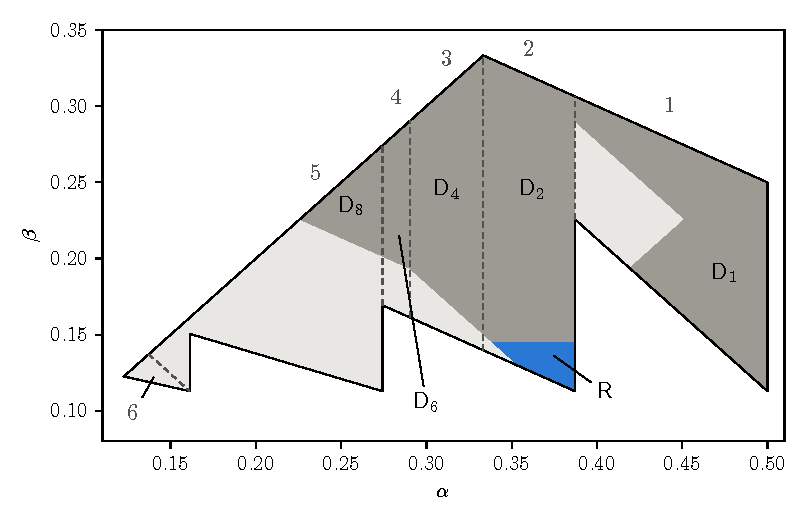
\includegraphics[width=0.8\textwidth]{../Code/figures/domain.pdf}
\caption{The domain $\mathsf{D}$ of \eqref{eq: domain} in the $(\alpha, \beta)$-plane at $\theta = 0.1129$. Dashed lines separate the ranges of Table~\ref{tab: ranges}, numbered $1$ to $6$: the vertical ones are at $\alpha = \sigma = 0.3871$, $1/3$, $\rho = 0.29032$ and $\sigma - \theta = 0.2742$, and the oblique one is the line $\alpha + \beta = \sigma - \theta$ between Ranges~$5$ and~$6$. Dark gray: the regions $\mathsf{D}_1$, $\mathsf{D}_2$, $\mathsf{D}_4$, $\mathsf{D}_6$ and $\mathsf{D}_8$ of Section~\ref{sec: decomposition}. Blue: the region $\mathsf{R}$ of \eqref{eq: region R}. Light gray: the rest of $\mathsf{D}$.}
\label{fig: domain}
\end{figure}

\subsection{\texorpdfstring{Groupings on the regions $\mathsf{R}$, $\mathsf{G}$ and $\mathsf{L}$}{Groupings on the regions R, G and L}}
\label{subsec: groupings}

Three groupings give asymptotic formulas to parts of the discarded sums. The grouping in Range~2 of the domain $\mathsf{D}$ of \eqref{eq: domain} (Table~\ref{tab: ranges}) acts on the region
\begin{equation}
\label{eq: region R}
\mathsf{R} := \bigl\{ 1/3 \Le \alpha < \sigma,\ \max(\zeta - \alpha, (\tau - \alpha)/2) \Le \beta \Le \rho/2 \bigr\}.
\end{equation}
Case (a) of \eqref{eq: lemma 12 cases} in Lemma~\ref{lem: lemma 13} applies the linear estimate to the factorization $(pq) \cdot r$, which needs $\alpha + \beta \Le \zeta$. On $\mathsf{R}$, where $\alpha + \beta \Ge \zeta$, case (b) applies it to the factorization $p \cdot (qr)$, which needs $\alpha \Le \zeta$, $2\beta \Le \rho$ and $\alpha + 2\beta \Le \nu$. In Range~2, $\alpha < \sigma < \zeta$ and $\sigma + \rho = \nu$, so these conditions reduce to $2\beta \Le \rho$, the upper limit of $\beta$ in \eqref{eq: region R}. The lower limits of $\beta$ there are $\zeta - \alpha$, below which case (a) applies, and $\beta_0(\alpha) = (\tau - \alpha)/2$. So on $\mathsf{R}$, identity \eqref{eq: identity 35} replaces the discard of the whole sum, and only its third sum is discarded, over $\mathsf{E}_{\mathsf{R}}$.

The other two groupings give parts of the third sums of \eqref{eq: identity 35} and \eqref{eq: identity 36} asymptotic formulas. On a region $\mathsf{G}$, the bilinear estimate applies to the products $pqrst$ with $s$ as its prime variable: \eqref{eq: bilinear exponents} holds with $x_{i_0} = \delta$ for a non-empty set $\mathcal{S} \subset \{p, q, r\}$. On a region $\mathsf{L}$, Buchstab's identity \eqref{eq: buchstab} at level $\mu^4$ writes $S(\mathcal{A}_{pqrs}, s)$ as the difference \eqref{eq: L split} of a sum sifted at level $\mu^4$ and a sum over a further prime $s' \prec s$. The sum over $s'$ enters with the sign $-$, so both sums need asymptotic formulas. The linear estimate treats the sum sifted at level $\mu^4$ on the region $\mathsf{I}$ where the primes $p, q, r, s$ satisfy $\alpha + \beta + \gamma + \delta \Le \tau$ or \eqref{eq: linear exponents}. Since $|s'|^2 \Le |s|^2$, the bilinear estimate with $s'$ as its prime variable treats the sum over $s'$ where \eqref{eq: bilinear exponents} holds with $x_{i_0} = \delta$ for a non-empty set $\mathcal{S} \subset \{p, q, r, s\}$. With an index set written by its primes, as in $x_{\{p, q\}} = \alpha + \beta$, these regions are
\begin{equation}
\label{eq: regions G L}
\begin{aligned}
\mathsf{G} &:= \bigcup_{\emptyset \neq \mathcal{S} \subset \{p, q, r\}} \bigl\{ \sigma \Le x_{\mathcal{S}} \Le \tau - \delta \bigr\}, \\
\mathsf{I} &:= \bigl\{ \alpha + \beta + \gamma + \delta \Le \tau \bigr\} \cup \bigcup_{\mathcal{U} \sqcup \mathcal{V} = \{p, q, r, s\}} \bigl\{ x_{\mathcal{U}} \Le \zeta,\ x_{\mathcal{V}} \Le \rho,\ \alpha + \beta + \gamma + \delta \Le \nu \bigr\}, \\
\mathsf{L} &:= \mathsf{I} \cap \bigcup_{\emptyset \neq \mathcal{S} \subset \{p, q, r, s\}} \bigl\{ \sigma \Le x_{\mathcal{S}} \Le \tau - \delta \bigr\}.
\end{aligned}
\end{equation}
Lemma~\ref{lem: four dim} proves the formulas on $\mathsf{G}$ and $\mathsf{L}$. These regions use the smallest prime of the product, $s$ or $s'$, as the prime variable of the bilinear estimate, and another prime in this role would not enlarge them. Indeed, let $x_0 \Le x_1$ be the exponents of the smallest prime of the product and of another prime $\varpi$ of the product, and let \eqref{eq: bilinear exponents} hold with $x_{i_0} = x_1$ for a set $\mathcal{S}$ of primes of the product with $\varpi \notin \mathcal{S}$. If $\mathcal{S}$ does not contain the smallest prime, then \eqref{eq: bilinear exponents} holds with $x_{i_0} = x_0$ for the same $\mathcal{S}$. If it does, replacing the smallest prime in $\mathcal{S}$ by $\varpi$ raises $x_{\mathcal{S}}$ by $x_1 - x_0$, to at least $\sigma$ and at most $\tau - x_0$.

The region $\mathsf{L}$ contains the polytope
\begin{equation}
\label{eq: polytope}
\mathsf{P} := \bigl\{ \alpha + \beta \Le \sigma,\ \gamma + \delta \Le \rho,\ \alpha + \beta + \delta \Ge \sigma,\ \alpha + \beta + 2\delta \Le \tau \bigr\}.
\end{equation}
On $\mathsf{P}$, the partition $\mathcal{U} = \{p, q\}$, $\mathcal{V} = \{r, s\}$ satisfies \eqref{eq: linear exponents}, since $\sigma < \zeta$ and $\sigma + \rho = \nu$, and the set $\mathcal{S} = \{p, q, s\}$ satisfies \eqref{eq: bilinear exponents} with $x_{i_0} = \delta$. Section~\ref{sec: numerics} also evaluates the losses with $\mathsf{P}$ in place of $\mathsf{L}$. Then $\mathsf{L}$ is replaced by a single polytope on which one partition and one set $\mathcal{S}$ serve every point, and the treatment of each four-dimensional box can be checked by hand.

\subsection{The total loss}
\label{subsec: total loss}

The lower bound of Lemma~\ref{lem: lower bound} drops the discarded sums over $\mathcal{A}$, and its main term is $2/(\pi W)$ times $S(\mathcal{B}, X^{1/2})$ minus the same sums over $\mathcal{B}$, as in \eqref{eq: lower bound boxes}. So each discarded sum is measured relative to $S(\mathcal{B}, X^{1/2})$. By Lemma~\ref{lem: boxes to integrals}, a discarded sum over $\mathcal{B}$ with exponents in a region, divided by $S(\mathcal{B}, X^{1/2})$, tends to the loss \eqref{eq: loss} of that region. For a two-dimensional region $\mathsf{F}$ and a four-dimensional region $\mathsf{F}'$, define the losses
\begin{equation}
\label{eq: loss}
\Phi(\mathsf{F}) := \iint_{\mathsf{F}} \omega\Bigl( \frac{1 - \alpha - \beta}{\beta} \Bigr) \frac{d\beta\, d\alpha}{\alpha \beta^2}, \qquad \Phi(\mathsf{F}') := \iiiint_{\mathsf{F}'} \omega\Bigl( \frac{1 - \alpha - \beta - \gamma - \delta}{\delta} \Bigr) \frac{d\delta\, d\gamma\, d\beta\, d\alpha}{\alpha \beta \gamma \delta^2},
\end{equation}
where $\omega$ is Buchstab's function, defined by $\omega(u) = 0$ for $u < 1$ and
\begin{equation}
\label{eq: buchstab function}
u\omega(u) = 1 + \int_1^{u-1} \omega(t)\, dt \qquad (u \Ge 1).
\end{equation}
This equation defines $\omega$ implicitly, starting from $\omega(u) = 1/u$ for $1 \Le u \Le 2$, where the integral vanishes.

Let $\Phi(\theta)$ be the total loss
\begin{equation}
\label{eq: total loss}
\Phi(\theta) := \sum_{k \in \{1, 2, 4, 6, 8\}} \Phi(\mathsf{D}_k) + \sum_{k \in \{3, \mathsf{R}, 5, 7, 9, 10, 11\}} \Phi\bigl(\mathsf{E}_k \setminus (\mathsf{G} \cup \mathsf{L})\bigr),
\end{equation}
with $\mathsf{D}_k$ of \eqref{eq: D1}, \eqref{eq: D2}, \eqref{eq: D4}, \eqref{eq: D6} and \eqref{eq: D8}, $\mathsf{E}_k$ of \eqref{eq: four dim regions}, and $\mathsf{G}$, $\mathsf{L}$ of \eqref{eq: regions G L}. Let $\Phi_{\mathsf{P}}(\theta)$ be defined in the same way with $\mathsf{P}$ in place of $\mathsf{L}$.

The total loss collects the losses of all sums that remain discarded: the sums over $(p, q)$ on the regions $\mathsf{D}_k$, and the third sums on the regions $\mathsf{E}_k$ outside $\mathsf{G} \cup \mathsf{L}$, where the groupings give asymptotic formulas. So $\Phi(\theta)$ measures the proportion of $S(\mathcal{B}, X^{1/2})$ that the discarded sums take up, and the lower bound of Lemma~\ref{lem: lower bound} is positive when $\Phi(\theta) < 1$.

Lemma~\ref{lem: lower bound} splits $\sum^*$ and the third sums into dyadic boxes. It applies Lemmas~\ref{lem: lemma 11}, \ref{lem: lemma 13}, \ref{lem: lemma 14} and~\ref{lem: four dim} to the boxes that lie inside a region where these lemmas apply, at distance at least $\varepsilon$ from its boundary, and it bounds the other boxes by Lemma~\ref{lem: boxes to integrals}. Section~\ref{sec: numerics} evaluates $\Phi(\theta)$ and shows $\Phi(0.1129) < 1$, which with Lemma~\ref{lem: lower bound} proves Theorem~\ref{thm: sector}.

\section{Asymptotic formulas from the linear and bilinear estimates}
\label{sec: estimates}

Each result of this section gives a sum an asymptotic formula in the sense of \eqref{eq: asymptotic formula}. Lemmas~\ref{lem: type I} and~\ref{lem: type II} below are the linear and bilinear estimates of Section~\ref{sec: outline}, in the form used in this paper. Appendix~\ref{app: arithmetic} derives them from the arithmetic information of \citet{harman2001gaussian}. The other results of this section give asymptotic formulas for sums in which the cofactor is sifted. Lemma~\ref{lem: fundamental} sifts it at levels up to $\mu^4$. Lemmas~\ref{lem: level large} and~\ref{lem: level small} sift the cofactors of the elements of $\mathcal{E}_n$ at a level $l(n)$ that depends on $n$. With Corollary~\ref{cor: level one}, they extend Lemmas~8, 9 and~10 of \citet{harman2001gaussian} (Appendix~\ref{app: comparison}). Appendix~\ref{app: sieve} contains the proofs of Lemmas~\ref{lem: fundamental}, \ref{lem: level large} and~\ref{lem: level small}.

\begin{lemma}
\label{lem: type I}
Let $c_v \Ge 0$ be divisor-bounded, and suppose that one of the following holds:
\begin{enumerate}[(a)]
\item $c_v$ is supported on $|v|^2 \Le X^{\tau} \mu^{-1}$;
\item $c_v = \sum_{v = uu'} a_u b_{u'}$, where $a_u, b_{u'} \Ge 0$ are divisor-bounded and supported on $u \sim U$, $u' \sim U'$, with $U \Le X^{\zeta} \mu^{-1}$, $U' \Le X^{\rho} \mu^{-1}$ and $UU' \Le X^{\nu} \mu^{-1}$.
\end{enumerate}
Then $\sum_{v \neq 0} c_v |\mathcal{E}_v|$ has an asymptotic formula \eqref{eq: asymptotic formula}.
\end{lemma}

The bilinear estimate of \citet[Lemma~5 and (30)]{harman2001gaussian} needs a prime variable. Its proof applies when the prime is restricted to any interval of norms above $\mu^4/2$ (Remark~\ref{rem: lemma 4 range}), and Section~\ref{sec: decoupling} restricts the prime to short intervals.

\begin{lemma}
\label{lem: type II}
Let $C_1 \Ge 1$, let $a_u, b_v \Ge 0$ be divisor-bounded and supported on $u \sim U$ and $v \sim V$ with $U, V \Ge W/C_1$, and let $\mu^4/2 \Le Z_1 < Z_2$. Then
\begin{equation}
\label{eq: type II}
\sum_{u \sim U,\ v \sim V} a_u b_v\, \#\{ \varpi : Z_1 \Le |\varpi|^2 < Z_2,\ uv\varpi \in \mathcal{E} \}
\end{equation}
has an asymptotic formula, uniformly in $U$, $V$, $Z_1$ and $Z_2$.
\end{lemma}

Lemma~\ref{lem: fundamental} below is a fundamental lemma over $\mathbb{Z}[i]$. Every level at which it is applied is at most $\mu^4 = X^{o(1)}$, so Brun's pure sieve suffices (Appendix~\ref{app: sieve}).

\begin{lemma}
\label{lem: fundamental}
Let $0 < \varepsilon_0 < 1$, let $c_u \Ge 0$ be divisor-bounded, and let $z_0$ be a function on the support of $c$ with $1 \Le z_0(u) \Le \mu^4$. Then $\sum_{u \neq 0} c_u S'(\mathcal{E}_u, z_0(u))$ has an asymptotic formula if one of the following holds:
\begin{enumerate}[(a)]
\item $c_u$ is supported on $|u|^2 \Le X^{\tau - \varepsilon_0} \mu^{-1}$;
\item $z_0$ is constant, and $c_u = \sum_{u = u_1 u_2} a_{u_1} b_{u_2}$, where $a_{u_1}, b_{u_2} \Ge 0$ are divisor-bounded and supported on $u_1 \sim U$, $u_2 \sim U'$, with $U \Le X^{\zeta} \mu^{-1}$, $U' \Le X^{\rho - \varepsilon_0} \mu^{-1}$ and $UU' \Le X^{\nu - \varepsilon_0} \mu^{-1}$.
\end{enumerate}
\end{lemma}

Lemma~\ref{lem: fundamental} sifts at levels up to $\mu^4$, and the decomposition needs levels $l(n)$ up to $X^{\tau}/|n|^2$. Lemmas~\ref{lem: level large} and~\ref{lem: level small} reach them through the bilinear estimate. Buchstab's identity \eqref{eq: buchstab} lowers the level $l(n)$ to $\mu^4$, where Lemma~\ref{lem: fundamental} applies, and subtracts a sum over a prime $q$ with $\mu^4 \Le |q|^2 < l(n)$. Once $q$ is confined to short intervals, $n$ is the variable $u$ of Lemma~\ref{lem: type II} in this sum, $q$ is its prime variable, and the cofactor $v$ of $nq$ satisfies $|v|^2 > (X/2)/(|n|^2 l(n))$. So Lemma~\ref{lem: type II} applies when $|n|^2 \Ge W/C_l$ and $l(n) \Le C_l X^{\tau}/|n|^2$, which are the hypotheses of Lemma~\ref{lem: level large}.

\begin{lemma}
\label{lem: level large}
Let $C_l \Ge 1$. Let $a_n \Ge 0$ be divisor-bounded and supported on $W/C_l \Le |n|^2 \Le X^{\tau - \varepsilon}$, and let $l$ be any function on the support of $a$ with $1 \Le l(n) \Le C_l X^{\tau}/|n|^2$. Then $\sum_{W/C_l \Le |n|^2 \Le X^{\tau - \varepsilon}} a_n S'(\mathcal{E}_n, l(n))$ has an asymptotic formula, uniformly in $a$ and $l$.
\end{lemma}

For $|n|^2 < W$, the variable $u = n$ is too small for Lemma~\ref{lem: type II}. The proof of Lemma~\ref{lem: level small} applies Buchstab's identity repeatedly, until the product of $n$ and the primes it introduces has norm at least $W$, and then applies Lemma~\ref{lem: level large} to that product. The bound $l(n) \Le C_l\, z(|n|^2)$, with $z$ of \eqref{eq: z function}, ensures that each such product and its level satisfy the hypotheses of Lemma~\ref{lem: level large}.

\begin{lemma}
\label{lem: level small}
Let $C_l \Ge 1$. Let $a_n \Ge 0$ be divisor-bounded and supported on $1 \Le |n|^2 < W$, and let $l$ be any function on the support of $a$ with $1 \Le l(n) \Le C_l\, z(|n|^2)$, with $z$ of \eqref{eq: z function}. Then $\sum_{1 \Le |n|^2 < W} a_n S'(\mathcal{E}_n, l(n))$ has an asymptotic formula, uniformly in $a$ and $l$.
\end{lemma}

\begin{corollary}
\label{cor: level one}
The sum $S(\mathcal{E}, X^{\theta})$ of \eqref{eq: identity 37} has an asymptotic formula.
\end{corollary}

\begin{proof}
The sum $S(\mathcal{E}, X^{\theta}) = S'(\mathcal{E}_1, X^{\theta})$ is the case $a_n = \mathbf{1}[n = 1]$, $l \equiv X^{\theta}$ of Lemma~\ref{lem: level small}. Its hypothesis holds, since $z(1) > X^{\theta}$ by \eqref{eq: z lower}.
\end{proof}

\section{Removing the conditions that couple the variables}
\label{sec: decoupling}

The sums of Harman's sieve run over products of primes with order constraints between them, conditions on products of their norms, and sieve conditions on the cofactor that depend on one of the primes. The bilinear estimate of Lemma~\ref{lem: type II} admits none of these conditions between its variables. This section removes them with short intervals. The order constraints and the conditions on products of norms are the cross-conditions of \citet[\S7]{merikoski2023polynomials}, and the short intervals give what he calls a finer-than-dyadic decomposition, which he builds from smooth weights \citep[\S3.1]{merikoski2023polynomials}. \citet[\S11.1]{heathbrown2017prime} separate variables by intervals $(A, A + A/L]$, of the same shape as ours, and \citet[p.~130]{harman2001gaussian} remove such conditions by Perron's formula (Appendix~\ref{app: comparison}). Every order constraint and every condition on a product of norms is constant on most Cartesian products of short intervals, and the sums over the other products are small. On a single Cartesian product, the sieve condition differs from sifting at a constant level only at the prime factors of the cofactor whose norms lie in a few short intervals. Lemma~\ref{lem: decoupling} reduces a sum with such conditions to sums over single Cartesian products of short intervals, and Lemma~\ref{lem: pieces} gives these sums asymptotic formulas under the conditions of Section~\ref{subsec: exponent form}. The sieve conditions sift the cofactor as $S'$ of \eqref{eq: cofactor sieve} does, at a level that may depend on the primes. The other terms defined below are introduced here, for the bookkeeping of this reduction.

Let $H := (\log X)^B$ with $B$ fixed, as in Lemma~\ref{lem: prime ideal theorem} of Appendix~\ref{app: arithmetic}, and put $\xi_\lambda := (1 + 1/H)^{\lambda}$ for integers $\lambda \Ge 0$. The \emph{short intervals} are $J_\lambda := [\xi_\lambda, \xi_{\lambda + 1})$. For a prime $q$, let $\lambda_q$ be the index with $|q|^2 \in J_{\lambda_q}$.

A \emph{configuration} $\mathcal{C}$ consists of the following data:
\begin{enumerate}[(i)]
\item prime variables $\varpi_1, \dots, \varpi_k$, with $k$ fixed and $|\varpi_i|^2 \in \mathcal{I}_i$ for intervals $\mathcal{I}_i \subset [\mu^4, X]$, the \emph{ranges} of the variables. A \emph{tuple} is a choice $\boldsymbol{\varpi} = (\varpi_1, \dots, \varpi_k)$ of these primes;
\item a cofactor $t$, which is a Gaussian integer;
\item finitely many \emph{monomial constraints} $c$, each of the form $m_c(\boldsymbol{\varpi}) < Z_c$ or $m_c(\boldsymbol{\varpi}) \Le Z_c$, where $m_c(\boldsymbol{\varpi}) := \prod_{i=1}^{k} |\varpi_i|^{2e_{c,i}}$ with integers $|e_{c,i}| \Le 2$, not all $0$, and $Z_c > 0$. We write $\mathbf{1}_c(\boldsymbol{\varpi})$ for the indicator that $\boldsymbol{\varpi}$ satisfies $c$. A lower bound $m_c(\boldsymbol{\varpi}) \Ge Z_c$ is the constraint $m_c(\boldsymbol{\varpi})^{-1} \Le Z_c^{-1}$. An order constraint $\varpi_i \prec \varpi_{i'}$ is the monomial constraint with $m_c(\boldsymbol{\varpi}) = |\varpi_i|^2/|\varpi_{i'}|^2$ and $Z_c = 1$, in which the case $m_c(\boldsymbol{\varpi}) = 1$ is decided by $\prec$;
\item a \emph{sieve condition} on $t$, with indicator $\Xi(\boldsymbol{\varpi}, t)$, of type (F), (C), (S) or (M): (F) none; (C) every prime factor of $t$ has norm at least $\mu^4$; (S) every prime factor $\varpi'$ of $t$ satisfies $\varpi' \succcurlyeq \varpi_{i_s}$, for a fixed index $i_s$; (M) every prime factor of $t$ has norm at least $m_s(\boldsymbol{\varpi}) := Z_s \prod_{i=1}^{k} |\varpi_i|^{2f_i}$, with $Z_s > 0$ and reals $|f_i| \Le 2$ that do not depend on the tuple.
\end{enumerate}
On every tuple that satisfies all the constraints, we require $\varpi_{i_s} \preccurlyeq \varpi_i$ for all $i$ in type (S), and $\mu^4 \Le m_s(\boldsymbol{\varpi}) \Le \min_i |\varpi_i|^2$ in type (M). The subscript $s$ of $i_s$, $m_s$ and $Z_s$ refers to the sieve condition, not to a prime $s$. The sum induced by $\mathcal{C}$ is
\begin{equation*}
\Sigma_{\mathcal{C}}(\mathcal{E}) := \sum_{\varpi_1, \dots, \varpi_k} \sum_{t \in \mathbb{Z}[i]} \mathbf{1}[\varpi_1 \cdots \varpi_k t \in \mathcal{E}] \prod_{i=1}^{k} \mathbf{1}[|\varpi_i|^2 \in \mathcal{I}_i] \prod_c \mathbf{1}_c(\boldsymbol{\varpi})\, \Xi(\boldsymbol{\varpi}, t).
\end{equation*}
A configuration has the type of its sieve condition, and we identify it with the sum $\Sigma_{\mathcal{C}}$ that it induces. For example, for fixed primes $p, q, r, s$, the sum $S'(\mathcal{E}_{pqrs}, s)$ counts the cofactors $t$ with $pqrst \in \mathcal{E}$ whose prime factors are all $\succcurlyeq s$. A sum of $S'(\mathcal{E}_{pqrs}, s)$ over primes in given ranges with $s \prec r \prec q \prec p$, such as a third sum of Section~\ref{subsec: decomposition}, is therefore a configuration with $k = 4$, the order constraints $s \prec r$, $r \prec q$ and $q \prec p$, and the sieve condition of type (S) with $i_s$ the index of $s$.

For an index vector $\boldsymbol{\lambda} = (\lambda_1, \dots, \lambda_k)$ of non-negative integers, let $\mathcal{T}(\boldsymbol{\lambda})$ be the set of tuples with $|\varpi_i|^2 \in \mathcal{I}_i \cap J_{\lambda_i}$ for all $i$. The \emph{pieces} of $\mathcal{C}$ are the sums over a single set $\mathcal{T}(\boldsymbol{\lambda})$, without constraints, in which the cofactor is sifted at a constant level $y \Ge 1$, or which have one further prime $\varpi'$ with norm in a short interval $J_{\lambda'}$ and a free cofactor:
\begin{equation}
\label{eq: pieces}
\mathcal{P}_{\boldsymbol{\lambda}}(\mathcal{E}; y) := \sum_{\boldsymbol{\varpi} \in \mathcal{T}(\boldsymbol{\lambda})} S'(\mathcal{E}_{\varpi_1 \cdots \varpi_k}, y), \qquad \mathcal{P}'_{\boldsymbol{\lambda},\lambda'}(\mathcal{E}) := \sum_{\boldsymbol{\varpi} \in \mathcal{T}(\boldsymbol{\lambda})} \sum_{|\varpi'|^2 \in J_{\lambda'}} |\mathcal{E}_{\varpi_1 \cdots \varpi_k \varpi'}|,
\end{equation}
where $\varpi'$ runs over primes and $\lambda' \Ge 0$ is an integer, the index of a single short interval, not an index vector like $\boldsymbol{\lambda}$. For $y = 1$ the cofactor of $\mathcal{P}_{\boldsymbol{\lambda}}(\mathcal{E}; y)$ is free, since $S'(\mathcal{E}_u, 1) = |\mathcal{E}_u|$.

The index vector $\boldsymbol{\lambda}$ \emph{satisfies} a constraint $c$ if every tuple of $\mathcal{T}(\boldsymbol{\lambda})$ satisfies $c$, and \emph{straddles} $c$ if $\mathcal{T}(\boldsymbol{\lambda})$ contains tuples that satisfy $c$ and tuples that do not. The \emph{level} of $\boldsymbol{\lambda}$ is
\begin{equation}
\label{eq: piece level}
y_{\boldsymbol{\lambda}} := \begin{cases} 1 & \text{in type (F)}, \\ \mu^4 & \text{in type (C)}, \\ \xi_{\lambda_{i_s}} & \text{in type (S)}, \\ \inf_{\mathcal{T}(\boldsymbol{\lambda})} m_s & \text{in type (M)}, \end{cases}
\end{equation}
and its \emph{window} is
\begin{equation}
\label{eq: window}
\mathcal{W}(\boldsymbol{\lambda}) := \begin{cases} \emptyset & \text{in types (F) and (C)}, \\ \{\lambda_{i_s}\} & \text{in type (S)}, \\ \{ \lambda' : J_{\lambda'} \cap [\inf_{\mathcal{T}(\boldsymbol{\lambda})} m_s, \sup_{\mathcal{T}(\boldsymbol{\lambda})} m_s) \neq \emptyset \} & \text{in type (M)}. \end{cases}
\end{equation}
Since $m_s$ varies by at most the factor $(1 + 1/H)^{2k}$ on $\mathcal{T}(\boldsymbol{\lambda})$, the window has at most $2k + 2$ elements. If $\boldsymbol{\lambda}$ satisfies all constraints, the requirements on types (S) and (M) give $y_{\boldsymbol{\lambda}} \Le \min_i |\varpi_i|^2$ on $\mathcal{T}(\boldsymbol{\lambda})$ and $\xi_{\lambda'} \Ge \mu^4/2$ for $\lambda' \in \mathcal{W}(\boldsymbol{\lambda})$. On the tuples of such an $\boldsymbol{\lambda}$, the sieve condition $\Xi(\boldsymbol{\varpi}, t)$ and sifting at the constant level $y_{\boldsymbol{\lambda}}$ differ only at the prime factors of $t$ with norm in $J_{\lambda'}$ for some $\lambda' \in \mathcal{W}(\boldsymbol{\lambda})$. So the part of $\Sigma_{\mathcal{C}}$ on the tuples of $\mathcal{T}(\boldsymbol{\lambda})$ differs from $\mathcal{P}_{\boldsymbol{\lambda}}(\mathcal{E}; y_{\boldsymbol{\lambda}})$ by at most the sum of $\mathcal{P}'_{\boldsymbol{\lambda},\lambda'}(\mathcal{E})$ over $\lambda' \in \mathcal{W}(\boldsymbol{\lambda})$.

\begin{lemma}
\label{lem: decoupling}
Let $\mathcal{C}$ be a configuration, and suppose that the following pieces \eqref{eq: pieces} have asymptotic formulas, uniformly in $\boldsymbol{\lambda}$ and $\lambda'$:
\begin{enumerate}[(a)]
\item $\mathcal{P}_{\boldsymbol{\lambda}}(\mathcal{E}; y_{\boldsymbol{\lambda}})$, with the level $y_{\boldsymbol{\lambda}}$ of \eqref{eq: piece level}, for every $\boldsymbol{\lambda}$ that satisfies all constraints;
\item $\mathcal{P}_{\boldsymbol{\lambda}}(\mathcal{E}; 1)$ for every $\boldsymbol{\lambda}$ that straddles some constraint;
\item $\mathcal{P}'_{\boldsymbol{\lambda},\lambda'}(\mathcal{E})$ for every $\boldsymbol{\lambda}$ that satisfies all constraints and every $\lambda'$ in its window $\mathcal{W}(\boldsymbol{\lambda})$ of \eqref{eq: window}.
\end{enumerate}
Then $\Sigma_{\mathcal{C}}$ has an asymptotic formula.
\end{lemma}

The pieces in (b) of Lemma~\ref{lem: decoupling} are the \emph{straddling pieces} of $\mathcal{C}$, and the pieces in (c) are its \emph{window pieces}. Summed over $\boldsymbol{\lambda}$ and $\lambda'$, the straddling and window pieces are small over $\mathcal{B}$, and their asymptotic formulas carry this bound to $\mathcal{A}$. Appendix~\ref{app: sieve} proves Lemma~\ref{lem: decoupling}.

The hypotheses of Lemma~\ref{lem: decoupling} are checked with Lemma~\ref{lem: pieces} below. A piece has the primes $\varpi_1, \dots, \varpi_K$, with $K = k$ for $\mathcal{P}_{\boldsymbol{\lambda}}(\mathcal{E}; y)$, and with $K = k + 1$ and $\varpi_{k+1} = \varpi'$ for $\mathcal{P}'_{\boldsymbol{\lambda},\lambda'}(\mathcal{E})$. Its cofactor $t$ is sifted at the constant level $y$, with $y = 1$ for $\mathcal{P}'_{\boldsymbol{\lambda},\lambda'}(\mathcal{E})$. The norm of $\varpi_i$ lies in $\Lambda_i$, and the \emph{exponents} of the piece are the $x_i$, where
\begin{equation*}
\Lambda_i := \mathcal{I}_i \cap J_{\lambda_i} \quad (i \Le k), \qquad \Lambda_{k+1} := J_{\lambda'}, \qquad x_i := \frac{\log \inf \Lambda_i}{\log X}.
\end{equation*}
Each $\Lambda_i$ lies in $[\mu^4/2, X]$ and has $\sup \Lambda_i \Le (1 + 1/H) \inf \Lambda_i$. So each $\log|\varpi_i|^2/\log X$ lies within $\mathcal{O}(1/(H \log X))$ of $x_i$, and a condition that holds at $(x_i)$ with margin $\varepsilon$ holds with margin $\varepsilon/2$ for every tuple of the piece, once $X$ is large. When the primes of a piece have names, an index set is written by its primes, as in $\mathcal{U} = \{p\}$, and $i_0$ by its prime, as in $\varpi_{i_0} = r$.

\begin{lemma}
\label{lem: pieces}
Let $C_1 \Ge 1$ be fixed. A piece \eqref{eq: pieces} has an asymptotic formula, uniformly in $\boldsymbol{\lambda}$ and $\lambda'$, if one of the following holds.
\begin{enumerate}[(P1)]
\item $y = 1$, and either $\sum_{i=1}^{K} x_i \Le \tau - \varepsilon$, or the indices split as $\mathcal{U} \sqcup \mathcal{V}$ with
\begin{equation*}
x_{\mathcal{U}} \Le \zeta - \varepsilon, \qquad x_{\mathcal{V}} \Le \rho - \varepsilon, \qquad \sum_{i=1}^{K} x_i \Le \nu - \varepsilon.
\end{equation*}
\item $y = \mu^4$, and the exponents satisfy one of the alternatives of (P1).
\item There are an index $i_0$ and a non-empty set $\mathcal{S}$ of other indices such that
\begin{equation*}
\inf \Bigl| \prod_{i \in \mathcal{S}} \varpi_i \Bigr|^2 \Ge \frac{W}{C_1}, \qquad \frac{X/2}{\sup |\varpi_{i_0} \prod_{i \in \mathcal{S}} \varpi_i|^2} \Ge \frac{W}{C_1},
\end{equation*}
with the infimum and the supremum over the tuples of the piece.
\item Every product $n = \varpi_1 \cdots \varpi_K$ of the piece satisfies
\begin{equation}
\label{eq: P4 large}
W/C_1 \Le |n|^2 \Le X^{\tau - \varepsilon}, \qquad y \Le C_1 X^{\tau}/|n|^2,
\end{equation}
or
\begin{equation}
\label{eq: P4 small}
|n|^2 < W, \qquad y \Le C_1\, z(|n|^2).
\end{equation}
\end{enumerate}
\end{lemma}

\begin{proof}
In (P1), the piece is $\sum_{v \neq 0} a_v |\mathcal{E}_v|$, where $a_v$ is the number of tuples of the piece with product $v$. This $a_v$ is non-negative, at most $d(v)^K$, and supported on $|v|^2 \Le X^{\sum_{i=1}^{K} x_i + o(1)}$. When the indices split as $\mathcal{U} \sqcup \mathcal{V}$, $a_v = \sum_{v = uu'} a'_u b_{u'}$, where $a'_u$ is the number of subtuples $(\varpi_i)_{i \in \mathcal{U}}$ with product $u$, and $b_{u'}$ is the number of subtuples $(\varpi_i)_{i \in \mathcal{V}}$ with product $u'$. Both $a'_u$ and $b_{u'}$ are supported on at most $2$ dyadic ranges. Lemma~\ref{lem: type I} applies, since the margin $\varepsilon/2$ absorbs the factor $\mu^{-1}$.

In (P2), the piece is $\sum_{u \neq 0} a_u S'(\mathcal{E}_u, \mu^4)$, where $a_u$ is the number of tuples of the piece with product $u$. Lemma~\ref{lem: fundamental} applies with $\varepsilon_0 = \varepsilon/4$: in case (a) when $\sum_{i=1}^{K} x_i \Le \tau - \varepsilon$, and in case (b) when the indices split as $\mathcal{U} \sqcup \mathcal{V}$, with $u_1$ and $u_2$ the products of the primes indexed by $\mathcal{U}$ and by $\mathcal{V}$, each in at most $2$ dyadic ranges.

In (P3), the piece is
\begin{equation*}
\sum_{u \neq 0,\ v \neq 0} a_u b_v\, \#\bigl\{ \varpi_{i_0} : |\varpi_{i_0}|^2 \in \Lambda_{i_0},\ uv\varpi_{i_0} \in \mathcal{E} \bigr\},
\end{equation*}
where $a_u$ is the number of subtuples $(\varpi_i)_{i \in \mathcal{S}}$ with product $u$, and $b_v$ is the number of pairs of a subtuple $(\varpi_i)_{i \notin \mathcal{S} \cup \{i_0\}}$ and a cofactor $t$ sifted at level $y$ with product $v$. Both are non-negative and divisor-bounded. The variable $u$ lies in at most $2$ dyadic ranges and $v$ in at most $4$. Both $|u|^2$ and $|v|^2$ are at least $W/C_1$. The norm of $\varpi_{i_0}$ ranges over $\Lambda_{i_0} \subset [\mu^4/2, X]$, so Lemma~\ref{lem: type II} applies.

In (P4), the piece is $\sum_{n \neq 0} a_n S'(\mathcal{E}_n, y)$, where $a_n$ counts the tuples with product $n$. Lemma~\ref{lem: level large} applies to the $n$ that satisfy \eqref{eq: P4 large} and Lemma~\ref{lem: level small} to those that satisfy \eqref{eq: P4 small}, both with the constant level $y$.
\end{proof}

\section{Sums over two primes}
\label{sec: two primes}

The lemmas of this section treat the sum $\sum^*$ of \eqref{eq: identity 37} on dyadic boxes. They supply the treatments of Table~\ref{tab: ranges}, and Section~\ref{sec: decomposition} checks their hypotheses on each range.

Throughout, $p \sim P$ and $q \sim Q$, where $P$ and $Q$ are powers of $2$. The pairs $(p, q)$ with $p \sim P$ and $q \sim Q$ form a \emph{box}. Its \emph{exponent rectangle} is the set of the pairs $(\alpha, \beta)$ with $X^{\alpha} \in [P, 2P)$ and $X^{\beta} \in [Q, 2Q)$, and the distance of a box from a set of exponents is that of its exponent rectangle. In every sifting function $S(\mathcal{A}_u, \cdot)$ below, every prime factor of $u$ satisfies the condition that defines the level, $|\varpi|^2 \Ge z$ or $\varpi \succcurlyeq q$, so $S(\mathcal{A}_u, \cdot) = S'(\mathcal{A}_u, \cdot)$ by the definition \eqref{eq: cofactor sieve} of $S'$. The sums and identities below are written for $\mathcal{A}$. Each sum is defined for $\mathcal{B}$ in the same way, and identities \eqref{eq: identity 35} and \eqref{eq: identity 36} hold with $\mathcal{B}$ in place of $\mathcal{A}$, since they follow from \eqref{eq: buchstab}.

Lemma~\ref{lem: lemma 11} gives the whole sum over a box an asymptotic formula, the treatment of Range~1 in Table~\ref{tab: ranges}. Its proof applies Buchstab's identity \eqref{eq: buchstab} at level $\mu^4$, the linear estimate to the sum sifted at this level, and the bilinear estimate, with $p$ as the variable $u$, to the sum that this identity subtracts.

\begin{lemma}
\label{lem: lemma 11}
Suppose that $W \Le P \Le X^{\zeta - \varepsilon}$, $Q \Ge P X^{-2\theta}$ and $PQ \Le X^{\nu - \varepsilon}$. Then the sum of $S(\mathcal{A}_{pq}, q)$ over $p \sim P$ and $q \sim Q$ has an asymptotic formula.
\end{lemma}

\begin{proof}
Since $Q \Le X^{\nu - \varepsilon}/W = X^{\rho - \varepsilon} < W \Le P$, the condition $q \prec p$ holds automatically. Buchstab's identity \eqref{eq: buchstab} at level $\mu^4$ gives
\begin{equation*}
\sum_{p \sim P,\, q \sim Q} S'(\mathcal{A}_{pq}, q) = \sum_{p \sim P,\, q \sim Q} S'(\mathcal{A}_{pq}, \mu^4) - \sum_{p \sim P,\, q \sim Q} \sum_{r \prec q,\ |r|^2 \Ge \mu^4} S'(\mathcal{A}_{pqr}, r).
\end{equation*}
The sum of $S'(\mathcal{A}_{pq}, \mu^4)$ is a configuration of type (C) without constraints. Its pieces fall under (P2) of Lemma~\ref{lem: pieces} with $\mathcal{U} = \{p\}$, $\mathcal{V} = \{q\}$ and $\varepsilon/2$ in place of $\varepsilon$, since $P \Le X^{\zeta - \varepsilon}$, $Q \Le X^{\rho - \varepsilon}$ and $PQ \Le X^{\nu - \varepsilon}$.

In the sum of $S'(\mathcal{A}_{pqr}, r)$, only the primes $r$ with $|r|^4 < X/(PQ)$ contribute. Indeed, for $|r|^4 \Ge X/(PQ)$, a cofactor $t \neq 1$ has $|t|^2 \Ge |r|^2$, so $|pqrt|^2 \Ge PQ |r|^4 \Ge X$. The cofactor $t = 1$ requires $|r|^2 \Ge X/(8PQ)$. Since $PQ^2 \Le X^{\nu + \rho - 2\varepsilon}$ and $\nu + \rho = (2 + 8\theta)/3 < 1$, this gives $|r|^2 > 2Q > |q|^2$, which contradicts $r \prec q$.
Hence the sum of $S'(\mathcal{A}_{pqr}, r)$ is the configuration with variables $p, q, r$, the range $[\mu^4, (X/(PQ))^{1/2})$ for $|r|^2$, the constraint $r \prec q$, and the sieve condition of type (S) with $i_s$ the index of $r$. Its requirement $r \preccurlyeq p$ holds, since $(X/(PQ))^{1/2} \Le X^{\tau}/P \Le X^{2\theta} < P$. All of its pieces, the window pieces included, fall under (P3) with $\mathcal{S} = \{p\}$ and $\varpi_{i_0} = r$. Indeed, $|p|^2 \Ge W$, and the quotient $(X/2)/\sup|pr|^2$ of (P3) satisfies
\begin{equation*}
\frac{X/2}{2P (X/(PQ))^{1/2} (1 + 1/H)} \Ge \frac{(XQ/P)^{1/2}}{5} \Ge \frac{W}{5},
\end{equation*}
since $Q \Ge P X^{-2\theta}$. Lemma~\ref{lem: decoupling} completes the proof.
\end{proof}

In the proof of Lemma~\ref{lem: lemma 13}, Lemma~\ref{lem: three primes} gives the sum over $(p, q, r)$ in \eqref{eq: identity 35} an asymptotic formula. The cases (a) and (b) of \eqref{eq: lemma 12 cases} correspond to the factorizations $(pq) \cdot r$ and $p \cdot (qr)$ of Section~\ref{subsec: groupings}.

\begin{lemma}
\label{lem: three primes}
Suppose that $Q \Le 2P$, $PQ \Ge W$ and $X^{\tau}/(PQ) \Ge X^{\varepsilon}$, and let $\mathcal{Q} \subset [Q, 2Q)$ and $\mathcal{I} \subset [X^{\tau}/(PQ), 2Q)$ be intervals with $\inf \mathcal{Q} \Ge X^{\tau}/(PQ)$. Then
\begin{equation}
\label{eq: lemma 12 sum}
\sum_{p \sim P,\ |q|^2 \in \mathcal{Q},\ q \prec p}\ \sum_{|r|^2 \in \mathcal{I},\ r \prec q} S\bigl(\mathcal{A}_{pqr}, X^{\tau}/(PQ)\bigr)
\end{equation}
has an asymptotic formula if one of the following holds:
\begin{equation}
\label{eq: lemma 12 cases}
\text{(a)}\ PQ \Le X^{\zeta - \varepsilon},\ Q \Le X^{\rho - \varepsilon},\ PQ^2 \Le X^{\nu - \varepsilon}; \qquad \text{(b)}\ P \Le X^{\zeta - \varepsilon},\ Q^2 \Le X^{\rho - \varepsilon},\ PQ^2 \Le X^{\nu - \varepsilon}.
\end{equation}
\end{lemma}

\begin{proof}
All of $p, q, r$ have norm at least $X^{\tau}/(PQ) \Ge X^{\varepsilon} \Ge \mu^4$, so Buchstab's identity \eqref{eq: buchstab} gives
\begin{equation*}
S\bigl(\mathcal{A}_{pqr}, X^{\tau}/(PQ)\bigr) = S'(\mathcal{A}_{pqr}, \mu^4) - \sum_{\mu^4 \Le |s|^2 < X^{\tau}/(PQ)} S'(\mathcal{A}_{pqrs}, s).
\end{equation*}
Summed as in \eqref{eq: lemma 12 sum}, the term $S'(\mathcal{A}_{pqr}, \mu^4)$ is the configuration with variables $p, q, r$, ranges $[P, 2P)$, $\mathcal{Q}$, $\mathcal{I}$, constraints $q \prec p$ and $r \prec q$, and the sieve condition of type (C). The sum of $S'(\mathcal{A}_{pqrs}, s)$ is the configuration with the further variable $s$, of range $[\mu^4, X^{\tau}/(PQ))$, the same constraints, and the sieve condition of type (S) with $i_s$ the index of $s$. Every tuple that satisfies the constraints has $s \prec r \prec q \prec p$, as type (S) requires. We apply Lemma~\ref{lem: decoupling} to both.

For the configuration of type (C), the pieces of hypothesis (a) of Lemma~\ref{lem: decoupling} fall under (P2), and the straddling pieces under (P1), with $\varepsilon/2$ in place of $\varepsilon$. There are no window pieces, since the window \eqref{eq: window} is empty in type (C). In case (a) of \eqref{eq: lemma 12 cases}, take $\mathcal{U} = \{p, q\}$ and $\mathcal{V} = \{r\}$: then $|pq|^2 < 4PQ$, $|r|^2 < 2Q$ and $|pqr|^2 < 8PQ^2$. In case (b), take $\mathcal{U} = \{p\}$ and $\mathcal{V} = \{q, r\}$: then $|p|^2 < 2P$, $|qr|^2 < 4Q^2$ and $|pqr|^2 < 8PQ^2$. In both cases \eqref{eq: lemma 12 cases} gives the conditions of (P1).

For the configuration of type (S), all pieces, the window pieces included, fall under (P3) with $\mathcal{S} = \{p, q\}$ and $\varpi_{i_0} = s$. Indeed, $|pq|^2 \Ge PQ \Ge W$. On every piece, $|s|^2 < (1 + 1/H) X^{\tau}/(PQ)$, so $(X/2)/\sup|pqs|^2 \Ge W/9$.
\end{proof}

For the boxes with $PQ \Ge W$, Lemma~\ref{lem: lemma 13} applies Buchstab's identity \eqref{eq: buchstab} twice at the level $X^{\tau}/(PQ)$.

\begin{lemma}
\label{lem: lemma 13}
Suppose that $X^{\varepsilon} \Le Q \Le 2P$ and $W \Le PQ \Le X^{\tau - \varepsilon}$. Split
\begin{equation*}
\sum_{p \sim P,\, q \sim Q,\, q \prec p} S(\mathcal{A}_{pq}, q) = S_< + S_\Ge
\end{equation*}
according as $|q|^2 < X^{\tau}/(PQ)$ or $|q|^2 \Ge X^{\tau}/(PQ)$. Then $S_<$ has an asymptotic formula, and
\begin{equation}
\label{eq: identity 35}
S_\Ge = \sum_{p, q} S\bigl(\mathcal{A}_{pq}, X^{\tau}/(PQ)\bigr) - \sum_{p, q}\ \sum_{\substack{r \prec q \\ |r|^2 \Ge X^{\tau}/(PQ)}} S\bigl(\mathcal{A}_{pqr}, X^{\tau}/(PQ)\bigr) + \sum_{p, q}\ \sum_{\substack{s \prec r \prec q \\ |s|^2 \Ge X^{\tau}/(PQ)}} S(\mathcal{A}_{pqrs}, s),
\end{equation}
where each $\sum_{p, q}$ runs over $p \sim P$, $q \sim Q$, $q \prec p$, $|q|^2 \Ge X^{\tau}/(PQ)$. If moreover (a) or (b) of \eqref{eq: lemma 12 cases} holds, then the sums in \eqref{eq: identity 35} over $(p, q)$ and over $(p, q, r)$ have asymptotic formulas.
\end{lemma}

\begin{proof}
Lemma~\ref{lem: decoupling} treats $S_<$, Lemma~\ref{lem: level large} the sum over $(p, q)$ in \eqref{eq: identity 35}, and Lemma~\ref{lem: three primes} the sum over $(p, q, r)$. For $n = pq$ with $p \sim P$ and $q \sim Q$,
\begin{equation}
\label{eq: lemma 13 pq}
W \Le |n|^2 < 4PQ \Le X^{\tau - \varepsilon/2}, \qquad \frac{X^{\tau}}{PQ} < \frac{4X^{\tau}}{|n|^2}.
\end{equation}
The sum $S_<$ is the configuration with variables $p, q$, ranges $[P, 2P)$ and $[Q, \min(2Q, X^{\tau}/(PQ)))$, the constraint $q \prec p$, and the sieve condition of type (S) with $i_s$ the index of $q$. In Lemma~\ref{lem: decoupling}, its pieces of hypothesis (a) have, by \eqref{eq: piece level}, the level $\xi_{\lambda_q} \Le |q|^2 < X^{\tau}/(PQ)$, and they fall under \eqref{eq: P4 large} of Lemma~\ref{lem: pieces} with $n = pq$ and $\varepsilon/2$ in place of $\varepsilon$, by \eqref{eq: lemma 13 pq}. Its straddling pieces, with $p$ and $q$ in the same short interval, fall under (P1) with $\varepsilon/2$ in place of $\varepsilon$, by \eqref{eq: lemma 13 pq}. Its window pieces, with $\varpi'$ in the short interval of $q$ by \eqref{eq: window}, fall under (P3) with $\mathcal{S} = \{p, q\}$ and $\varpi_{i_0} = \varpi'$, since $|pq|^2 \Ge W$ and $|pq\varpi'|^2 < 4(1 + 1/H) X^{\tau}$, so that $(X/2)/\sup|pq\varpi'|^2 \Ge W/9$.

For $|q|^2 \Ge X^{\tau}/(PQ)$, Buchstab's identity \eqref{eq: buchstab}, applied first to $S(\mathcal{A}_{pq}, q)$ and then to each $S(\mathcal{A}_{pqr}, r)$ with $|r|^2 \Ge X^{\tau}/(PQ)$, gives \eqref{eq: identity 35}. The sum over $(p, q)$ in \eqref{eq: identity 35} is $\sum_{n \neq 0} a_n S(\mathcal{A}_n, X^{\tau}/(PQ))$, with $n = pq$ and $a_n$ the number of pairs $(p, q)$ in the range of $\sum_{p, q}$ with $pq = n$. Lemma~\ref{lem: level large} applies to it with $\varepsilon/2$ in place of $\varepsilon$, by \eqref{eq: lemma 13 pq}. The sum over $(p, q, r)$ is the case $\mathcal{Q} = [\max(Q, X^{\tau}/(PQ)), 2Q)$ and $\mathcal{I} = [X^{\tau}/(PQ), 2Q)$ of Lemma~\ref{lem: three primes}, whose hypothesis $X^{\tau}/(PQ) \Ge X^{\varepsilon}$ holds because $PQ \Le X^{\tau - \varepsilon}$.
\end{proof}

For the boxes with $PQ < W$, the level $X^{\tau}/(PQ)$ of \eqref{eq: identity 35} exceeds $z(PQ)$, the level that Lemma~\ref{lem: level small} admits up to a constant factor, and Lemma~\ref{lem: lemma 14} applies Buchstab's identity \eqref{eq: buchstab} at levels given by $z$ instead.

\begin{lemma}
\label{lem: lemma 14}
Let $j \in \{0, 1\}$ and $0 < 4\varepsilon < 5\theta/2 - 1/4$. Suppose that $X^{\varepsilon} \Le Q \Le 2P$ and $W X^{-(j+1)\theta} \Le PQ < W X^{-j\theta}$, so that $j(PQ) = j$ and $z(PQ) = (X^{\tau}/(PQ))^{1/(j+2)}$. Split
\begin{equation*}
\sum_{p \sim P,\, q \sim Q,\, q \prec p} S(\mathcal{A}_{pq}, q) = S_< + S_\Ge
\end{equation*}
according as $|q|^2 < z(PQ)$ or $|q|^2 \Ge z(PQ)$. Then $S_<$ has an asymptotic formula, and
\begin{equation}
\label{eq: identity 36}
\begin{aligned}
S_\Ge = {} & \sum_{p, q} S\bigl(\mathcal{A}_{pq}, z(PQ)\bigr) - \sum_{p, q} \sum_{\substack{r \prec q \\ |r|^2 \Ge z(PQ)}} S\Bigl(\mathcal{A}_{pqr}, \Bigl(\frac{X^{\tau}}{PQ|r|^2}\Bigr)^{1/(j+1)}\Bigr) \\
& + \sum_{p, q} \sum_{\substack{r \prec q \\ |r|^2 \Ge z(PQ)}} \sum_{\substack{s \prec r \\ |s|^{2(j+1)} \Ge X^{\tau}/(PQ|r|^2)}} S(\mathcal{A}_{pqrs}, s),
\end{aligned}
\end{equation}
where each $\sum_{p, q}$ runs over $p \sim P$, $q \sim Q$, $q \prec p$, $|q|^2 \Ge z(PQ)$. The sums in \eqref{eq: identity 36} over $(p, q)$ and over $(p, q, r)$ have asymptotic formulas.
\end{lemma}

\begin{proof}
We first derive \eqref{eq: identity 36} and prove the bounds \eqref{eq: lemma 14 small products} to \eqref{eq: lemma 14 pq levels}. With these bounds, Lemmas~\ref{lem: level large} and~\ref{lem: level small} give the sum over $(p, q)$ in \eqref{eq: identity 36} an asymptotic formula. Lemma~\ref{lem: decoupling} gives $S_<$ and the sum over $(p, q, r)$ asymptotic formulas: the pieces of its hypothesis (a) fall under (P4) of Lemma~\ref{lem: pieces}, and the straddling and window pieces under (P1) or (P3).

For $|q|^2 \Ge z(PQ)$, Buchstab's identity \eqref{eq: buchstab} gives
\begin{equation*}
S(\mathcal{A}_{pq}, q) = S\bigl(\mathcal{A}_{pq}, z(PQ)\bigr) - \sum_{\substack{r \prec q \\ |r|^2 \Ge z(PQ)}} S(\mathcal{A}_{pqr}, r).
\end{equation*}
For such $r$, $|r|^{2(j+2)} \Ge z(PQ)^{j+2} = X^{\tau}/(PQ)$, so the level of the sum over $(p, q, r)$ in \eqref{eq: identity 36}, which serves as the function $m_s$ of a sieve condition of type (M) of Section~\ref{sec: decoupling}, satisfies
\begin{equation}
\label{eq: lemma 14 ms}
m_s(p, q, r) := \Bigl( \frac{X^{\tau}}{PQ|r|^2} \Bigr)^{1/(j+1)} \Le |r|^2.
\end{equation}
So \eqref{eq: buchstab} applies again to $S(\mathcal{A}_{pqr}, r)$, at the level $m_s(p, q, r)$, and \eqref{eq: identity 36} follows.

For a prime $q'$ with $|q'|^2 \Le 4Q$, which below is $r$ or the prime $\varpi'$ of a window piece, the bounds $Q^2 \Le 2PQ$ and $PQ < W$ give $|pqq'|^2 < 16PQ^2 < 32 (PQ)^{3/2} < 32 X^{3\sigma/2}$. Since $3\sigma/2 = \tau - (5\theta/2 - 1/4)$ and $4\varepsilon < 5\theta/2 - 1/4$,
\begin{equation}
\label{eq: lemma 14 small products}
|pq|^2 |q'|^2 \Le X^{\tau - 3\varepsilon} \qquad (|q'|^2 \Le 4Q).
\end{equation}
If $|r|^2 \Ge z(PQ)$, then $|pqr|^2 \Ge PQ\, z(PQ) = (PQ)^{(j+1)/(j+2)} X^{\tau/(j+2)}$, and $PQ \Ge W X^{-(j+1)\theta}$ gives
\begin{equation}
\label{eq: lemma 14 three primes}
|pqr|^2 \Ge W X^{\theta/2} \quad (j = 0), \qquad |pqr|^2 \Ge W X^{-2\theta/3} \quad (j = 1).
\end{equation}
For $|r|^2 < 2Q$, the level \eqref{eq: lemma 14 ms} satisfies
\begin{equation}
\label{eq: lemma 14 level}
m_s(p, q, r) \Ge \Bigl( \frac{X^{\tau}}{8PQ^2} \Bigr)^{1/(j+1)} \Ge \frac{X^{(\tau - 3\sigma/2)/2}}{8} \Ge X^{2\varepsilon} \Ge \mu^4.
\end{equation}

Let $n = pq$ with $p \sim P$ and $q \sim Q$. Then $|n|^2 \Ge PQ \Ge W X^{-(j+1)\theta}$, so $j(|n|^2) \Le j$ if $|n|^2 < W$. Also $|n|^2 < 4PQ < 4W X^{-j\theta}$, so $|n|^2 \Ge W$ only for $j = 0$, and then $|n|^2 < 4W \Le X^{\tau - \varepsilon}$. Hence
\begin{equation}
\label{eq: lemma 14 pq levels}
\begin{aligned}
z(|n|^2) &\Ge \Bigl( \frac{X^{\tau}}{4PQ} \Bigr)^{1/(j+2)} > \frac{z(PQ)}{4} && (|n|^2 < W), \\
z(PQ) &= \Bigl( \frac{X^{\tau}}{PQ} \Bigr)^{1/2} \Le \frac{X^{\tau}}{4PQ} \Le \frac{X^{\tau}}{|n|^2} && (|n|^2 \Ge W).
\end{aligned}
\end{equation}

The sum over $(p, q)$ in \eqref{eq: identity 36} is $\sum_{n \neq 0} a_n S(\mathcal{A}_n, z(PQ))$, with $n = pq$ and $a_n$ the number of pairs $(p, q)$ in the range of $\sum_{p, q}$ with $pq = n$. By \eqref{eq: lemma 14 pq levels}, Lemma~\ref{lem: level small} applies to the $n$ with $|n|^2 < W$, and Lemma~\ref{lem: level large} to the others, both with the constant level $z(PQ)$.

The sum $S_<$ is the configuration with variables $p, q$, ranges $[P, 2P)$ and $[Q, \min(2Q, z(PQ)))$, the constraint $q \prec p$, and the sieve condition of type (S) with $i_s$ the index of $q$. In Lemma~\ref{lem: decoupling}, its pieces of hypothesis (a) have, by \eqref{eq: piece level}, the level $y = \xi_{\lambda_q} \Le |q|^2 < z(PQ)$, and they fall under (P4) with $n = pq$ by \eqref{eq: lemma 14 pq levels}. Its straddling pieces and window pieces fall under (P1) by \eqref{eq: lemma 14 small products}.

The sum over $(p, q, r)$ in \eqref{eq: identity 36} is the configuration with variables $p, q, r$, constraints $q \prec p$ and $r \prec q$, the ranges $[P, 2P)$, $[\max(Q, z(PQ)), 2Q)$ and $[z(PQ), 2Q)$, and the sieve condition of type (M) with the level $m_s(p, q, r)$ of \eqref{eq: lemma 14 ms}. Its requirement $\mu^4 \Le m_s(p, q, r) \Le |r|^2$ holds by \eqref{eq: lemma 14 ms} and \eqref{eq: lemma 14 level}. In Lemma~\ref{lem: decoupling}, a piece of hypothesis (a) has, by \eqref{eq: piece level}, the level $y = \inf m_s$ over the piece. Every product $n = pqr$ of the piece has $|n|^2 < 4PQ|r|^2$, so
\begin{equation*}
y \Le m_s(p, q, r) < \Bigl( \frac{4X^{\tau}}{|n|^2} \Bigr)^{1/(j+1)}.
\end{equation*}
For $j = 0$, every $n$ has $W \Le |n|^2 \Le X^{\tau - 3\varepsilon}$ by \eqref{eq: lemma 14 three primes} and \eqref{eq: lemma 14 small products}, so the piece falls under \eqref{eq: P4 large}. For $j = 1$, an $n$ with $|n|^2 \Ge W$ has $|n|^2 \Le X^{\tau - 3\varepsilon}$ by \eqref{eq: lemma 14 small products} and $y \Le y^2 < 4X^{\tau}/|n|^2$, which is \eqref{eq: P4 large}. An $n$ with $|n|^2 < W$ has $|n|^2 \Ge W X^{-2\theta/3}$ by \eqref{eq: lemma 14 three primes}, so $j(|n|^2) = 0$ and $y < 2(X^{\tau}/|n|^2)^{1/2} = 2z(|n|^2)$, which is \eqref{eq: P4 small}.

The straddling pieces fall under (P1) by \eqref{eq: lemma 14 small products}. A window piece adds a prime $\varpi'$ with $|\varpi'|^2$ within the factor $(1 + 1/H)^2$ of $m_s(p, q, r)$, by \eqref{eq: window}. For $j = 1$ it falls under (P1), because $|pqr\varpi'|^2 \Le 8(X^{\tau} |pqr|^2)^{1/2} \Le X^{\tau - \varepsilon}$ by \eqref{eq: lemma 14 small products}. For $j = 0$ it falls under (P3) with $\mathcal{S} = \{p, q, r\}$ and $\varpi_{i_0} = \varpi'$. Indeed, $|pqr|^2 \Ge W$ by \eqref{eq: lemma 14 three primes}, and $|pqr\varpi'|^2 \Le 5X^{\tau}$ on the piece, so $(X/2)/\sup|pqr\varpi'|^2 \Ge W/10$.
\end{proof}

\section{The ranges and the discarded regions}
\label{sec: decomposition}

This section proves identity \eqref{eq: identity 37}, defines the regions of Table~\ref{tab: ranges}, and checks the treatment of each range.

\begin{lemma}
\label{lem: identity 37}
Let $\Pi_1$, $\Pi_2$ and $\sum^*$ be as in Section~\ref{sec: outline}. Identity \eqref{eq: identity 37} holds for $\mathcal{E} \in \{\mathcal{A}, \mathcal{B}\}$. The terms on the right of \eqref{eq: identity 37} other than $\sum^*$ have asymptotic formulas. A prime $p$ with $|p|^2 = X^{\alpha}$ lies in $\Pi_2$ exactly when $\theta \Le \alpha < \tau/5$ or $\sigma - 2\theta \Le \alpha < \tau/4$. The interval $[\sigma - 2\theta, \tau/4)$ is empty for $\theta \Le 3/26$.
\end{lemma}

\begin{proof}
Buchstab's identity \eqref{eq: buchstab} gives
\begin{equation*}
S(\mathcal{E}, X^{1/2}) = S(\mathcal{E}, X^{\theta}) - \sum_{X^{\theta} \Le |p|^2 < X^{1/2}} S(\mathcal{E}_p, p),
\end{equation*}
and $S(\mathcal{E}_p, p) = S'(\mathcal{E}_p, p)$. For $p \in \Pi_1$, the identity of \eqref{eq: buchstab} for $S'(\mathcal{E}_u, q)$, with $u = q = p$ and $w = z(|p|^2) \Le |p|^2$, gives
\begin{equation*}
S'(\mathcal{E}_p, p) = S\bigl(\mathcal{E}_p, z(|p|^2)\bigr) - \sum_{\substack{q \prec p \\ |q|^2 \Ge z(|p|^2)}} S(\mathcal{E}_{pq}, q).
\end{equation*}
Together they give \eqref{eq: identity 37}.

The term $S(\mathcal{E}, X^{\theta})$ of \eqref{eq: identity 37} has an asymptotic formula by Corollary~\ref{cor: level one}. In the sum of $S(\mathcal{E}_p, z(|p|^2))$ over $p \in \Pi_1$, the level $z(|p|^2)$ does not exceed $|p|^2$, so $S = S'$. For $|p|^2 \Ge W$ the level is $X^{\tau}/|p|^2$ and $|p|^2 < X^{1/2} = X^{\tau - \theta}$, so Lemma~\ref{lem: level large} applies. For $|p|^2 < W$, Lemma~\ref{lem: level small} applies with the level $z(|p|^2)$.

In the sum over $p \in \Pi_2$, the term $S(\mathcal{E}_p, p)$ differs from $S'(\mathcal{E}_p, |p|^2)$ only by the cofactors divisible by the other prime $p'$ of norm $|p|^2$, when it exists and $p' \prec p$. So $0 \Le S'(\mathcal{E}_p, |p|^2) - S(\mathcal{E}_p, p) \Le |\mathcal{E}_{pp'}|$. For $p \in \Pi_2$, $|p|^2 < z(|p|^2)$ and $|p|^2 < W$, so Lemma~\ref{lem: level small} gives the sum of $S'(\mathcal{E}_p, |p|^2)$ over $p \in \Pi_2$ an asymptotic formula. Since $|pp'|^2 = |p|^4 < X^{\tau/2}$, Lemmas~\ref{lem: type I}(a) and~\ref{lem: counting}(a) give
\begin{equation*}
\sum_{p \in \Pi_2} |\mathcal{A}_{pp'}| = \frac{2}{\pi W} \sum_{p \in \Pi_2} |\mathcal{B}_{pp'}| + \mathcal{O}\bigl(XW^{-1}(\log X)^{-A}\bigr), \qquad \sum_{p \in \Pi_2} |\mathcal{B}_{pp'}| \ll X \sum_{|p|^2 \Ge X^{\theta}} |p|^{-4} \ll X^{1 - \theta}.
\end{equation*}
So the sums of $|\mathcal{A}_{pp'}|$ and of $2|\mathcal{B}_{pp'}|/(\pi W)$ over $p \in \Pi_2$ are $\mathcal{O}(XW^{-1}(\log X)^{-A})$, and the sum of $S(\mathcal{E}_p, p)$ over $p \in \Pi_2$ has an asymptotic formula.

By the definition of $\beta_0$, a prime $p$ with $|p|^2 = X^{\alpha}$ and $\theta \Le \alpha < 1/2$ lies in $\Pi_2$ exactly when $\beta_0(\alpha) > \alpha$. For $\alpha \Ge \sigma$, $\beta_0(\alpha) = \tau - \alpha \Le \alpha$. For $\alpha < \sigma$ and $j = j(X^{\alpha})$, the inequality $\beta_0(\alpha) > \alpha$ means $\alpha < \tau/(j+3)$. For $j = 0$ this is impossible, because $j = 0$ gives $\alpha \Ge \sigma - \theta > \tau/3$. For $j = 1$ it gives $\alpha \in [\sigma - 2\theta, \tau/4)$, and $\tau/4 \Le \sigma - 2\theta$ for $\theta \Le 3/26$. For $j = 2$ it gives $\theta \Le \alpha < \tau/5$, since $\theta > \sigma - 3\theta$ and $\tau/5 < \sigma - 2\theta$. For $j \Ge 3$, $\alpha < \sigma - 3\theta < \theta$, which is excluded.
\end{proof}

At $\theta = 0.1129$ the primes of $\Pi_2$ have $\alpha \in [0.1129, 0.12258)$, so $\mathsf{D}$ begins at $\alpha = \tau/5 = 0.12258$ in Figure~\ref{fig: domain}.

In the sum $\sum^*$, a term with $|p|^2 |q|^4 \Ge X$ has cofactor $t = 1$, because a cofactor $t \neq 1$ has $|t|^2 \Ge |q|^2$ and would give $|pqt|^2 \Ge |p|^2 |q|^4 \Ge X$. Then $pq \in \mathcal{E}$ and $q \prec p$ force $|p|^4 \Ge X/2$ and $|q|^2 \Ge X^{1/2}/2$, and the number of such pairs with $pq \in \mathcal{B}$ is $\mathcal{O}(X/(\log X)^2)$. These terms are non-negative and enter \eqref{eq: identity 37} with the sign $+$, so we discard them. Their contribution tends to $0$ after division by $S(\mathcal{B}, X^{1/2})$, which is of order $X/\log X$ by \eqref{eq: primes in B}. The remaining pairs have exponents in the domain $\mathsf{D}$ of \eqref{eq: domain}.

On each part of Ranges~1 to~6, the hypotheses of the lemmas used there are linear inequalities in $\alpha$, $\beta$ and $\theta$. Appendix~\ref{app: inequalities} lists the inequalities between the parameters that these hypotheses use, with their values at $\theta = 0.1129$. On each range, the discarded region consists of the pairs on which no lemma of Section~\ref{sec: two primes} applies.

Range~1 consists of the pairs with $\sigma \Le \alpha < 1/2$. Here $\beta_0(\alpha) = \tau - \alpha$ and $\beta < (1 - \alpha)/2 < \alpha$. Lemma~\ref{lem: lemma 11} gives an asymptotic formula where $\alpha \Le \zeta$, $\beta \Ge \alpha - 2\theta$ and $\alpha + \beta \Le \nu$. The discarded region is
\begin{equation}
\label{eq: D1}
\mathsf{D}_1 := \bigl\{ \sigma \Le \alpha < 1/2,\ \tau - \alpha \Le \beta < (1 - \alpha)/2 \bigr\} \setminus \bigl\{ \alpha - 2\theta \Le \beta \Le \nu - \alpha \bigr\}.
\end{equation}
The set subtracted in $\mathsf{D}_1$ is empty for $\alpha > \chi$, where $\chi := (\nu + 2\theta)/2$. Since $\chi < \zeta$, the condition $\alpha \Le \zeta$ of Lemma~\ref{lem: lemma 11} holds wherever this set is non-empty. The exponent $\chi$ is that of the hypothesis $P \ll X^{\chi}$ of Lemma~11 of \citet{harman2001gaussian} (Appendix~\ref{app: comparison}).

Range~2 consists of the pairs with $1/3 \Le \alpha < \sigma$. Here $j(X^{\alpha}) = 0$, so $\beta_0(\alpha) = (\tau - \alpha)/2$, and $\beta < (1 - \alpha)/2$. Lemma~\ref{lem: lemma 13} applies in case (a) of \eqref{eq: lemma 12 cases} where $\alpha + \beta \Le \zeta$, since there $\beta \Le \zeta - 1/3 < \rho$ and $\alpha + 2\beta \Le 2\zeta - 1/3 < \nu$. It applies in case (b) on the region $\mathsf{R}$ of \eqref{eq: region R}, since there $\alpha < \sigma < \zeta$, $2\beta \Le \rho$, $\alpha + 2\beta < \sigma + \rho = \nu$ and $\alpha + \beta < \sigma + \rho/2 < \tau$. In both cases $\alpha + \beta \Ge (\alpha + \tau)/2 > \sigma$ and $\beta \Ge (\tau - \alpha)/2$, so $PQ \Ge W$ and $S_< = 0$. Where Lemma~\ref{lem: lemma 13} applies, only the third sum of \eqref{eq: identity 35} is discarded. The two-dimensional discarded region is
\begin{equation}
\label{eq: D2}
\mathsf{D}_2 := \bigl\{ 1/3 \Le \alpha < \sigma,\ \max(\zeta - \alpha, (\tau - \alpha)/2) \Le \beta < (1 - \alpha)/2,\ \beta > \rho/2 \bigr\}.
\end{equation}

Range~3 consists of the pairs with $\rho \Le \alpha < 1/3$. Here $\beta_0(\alpha) = (\tau - \alpha)/2$ and $\beta < \alpha$. Lemma~\ref{lem: lemma 13} applies in case (a) where $\alpha + \beta \Le \zeta$, since there $\beta \Le \zeta - \rho < \rho$, $\alpha + 2\beta \Le 2\zeta - \rho = \nu$ and $\alpha + \beta \Ge (\rho + \tau)/2 > \sigma$. The discarded region is
\begin{equation}
\label{eq: D4}
\mathsf{D}_4 := \bigl\{ \rho \Le \alpha < 1/3,\ \zeta - \alpha \Le \beta < \alpha \bigr\}.
\end{equation}

Range~4 consists of the pairs with $\sigma - \theta \Le \alpha < \rho$. Here $\beta_0(\alpha) = (\tau - \alpha)/2$. Lemma~\ref{lem: lemma 13} applies in case (a) where $\alpha + 2\beta \Le \nu$, since there $\alpha + \beta \Le (\alpha + \nu)/2 < (\rho + \nu)/2 = \zeta$, $\beta \Le (\nu - \sigma + \theta)/2 = (\rho + \theta)/2 < \rho$ and $\alpha + \beta \Ge (\alpha + \tau)/2 \Ge (1 - \theta)/2 > \sigma$. The discarded region is
\begin{equation}
\label{eq: D6}
\mathsf{D}_6 := \bigl\{ \sigma - \theta \Le \alpha < \rho,\ (\nu - \alpha)/2 \Le \beta < \alpha \bigr\}.
\end{equation}

Range~5 consists of the pairs with $\alpha < \sigma - \theta$ and $\alpha + \beta \Ge \sigma - \theta$. Here $j(X^{\alpha}) \Ge 1$, so $\beta_0(\alpha) \Le (\tau - \alpha)/3$, and pairs with $\beta < (\tau - \alpha)/2$ occur. Where $\alpha + \beta \Ge \sigma$ and $\beta < (\tau - \alpha)/2$, the sum equals $S_<$ of Lemma~\ref{lem: lemma 13} and has an asymptotic formula. Where $\alpha + \beta \Ge \sigma$, $\beta \Ge (\tau - \alpha)/2$ and $\alpha + 2\beta \Le \nu$, Lemma~\ref{lem: lemma 13} applies in case (a), since there $\beta < \alpha < \sigma - \theta < \rho$ and $\alpha + \beta \Le (\alpha + \nu)/2 < (\sigma - \theta + \nu)/2 < \zeta$. Where $\alpha + \beta < \sigma$, $j(X^{\alpha + \beta}) = 0$, and Lemma~\ref{lem: lemma 14} with $j = 0$ applies. The discarded region is
\begin{equation}
\label{eq: D8}
\mathsf{D}_8 := \bigl\{ \nu/3 \Le \alpha < \sigma - \theta,\ (\nu - \alpha)/2 \Le \beta < \alpha \bigr\}.
\end{equation}

Range~6 consists of the pairs with $\alpha + \beta < \sigma - \theta$. Since $p \in \Pi_1$, Lemma~\ref{lem: identity 37} gives $\alpha \Ge \tau/5 > \sigma - 3\theta$, so $j(X^{\alpha}) \Le 2$ and $\beta \Ge \beta_0(\alpha) \Ge (\tau - \alpha)/4$. Hence $\alpha + \beta \Ge (3\alpha + \tau)/4 \Ge 2\tau/5 > \sigma - 2\theta$, so $j(X^{\alpha + \beta}) = 1$, and Lemma~\ref{lem: lemma 14} with $j = 1$ applies. Since $\beta \Ge (\tau - \alpha)/4$ is equivalent to $|q|^2 \Ge z(|pq|^2)$, $S_< = 0$ on every box at distance at least $\varepsilon$ from the boundary of $\mathsf{D}$.

In the third sum of \eqref{eq: identity 35}, the exponents satisfy $\tau - \alpha - \beta \Le \delta < \gamma < \beta$. In that of \eqref{eq: identity 36}, they satisfy
\begin{equation*}
\frac{\tau - \alpha - \beta}{j + 2} \Le \gamma < \beta, \qquad \frac{\tau - \alpha - \beta - \gamma}{j + 1} \Le \delta < \gamma.
\end{equation*}
With these limits, the third sums are discarded over the following regions of $(\alpha, \beta, \gamma, \delta)$:
\begin{equation}
\label{eq: four dim regions}
\begin{aligned}
\mathsf{E}_3 &: 1/3 \Le \alpha < \sigma,\ (\tau - \alpha)/2 \Le \beta \Le \zeta - \alpha,\ \tau - \alpha - \beta \Le \delta < \gamma < \beta; \\
\mathsf{E}_{\mathsf{R}} &: (\alpha, \beta) \in \mathsf{R},\ \tau - \alpha - \beta \Le \delta < \gamma < \beta; \\
\mathsf{E}_5 &: \rho \Le \alpha < 1/3,\ (\tau - \alpha)/2 \Le \beta \Le \zeta - \alpha,\ \tau - \alpha - \beta \Le \delta < \gamma < \beta; \\
\mathsf{E}_7 &: \sigma - \theta \Le \alpha < \rho,\ (\tau - \alpha)/2 \Le \beta \Le (\nu - \alpha)/2,\ \tau - \alpha - \beta \Le \delta < \gamma < \beta; \\
\mathsf{E}_9 &: \alpha < \sigma - \theta,\ (\tau - \alpha)/2 \Le \beta \Le \min((\nu - \alpha)/2, \alpha),\ \tau - \alpha - \beta \Le \delta < \gamma < \beta; \\
\mathsf{E}_{10} &: \tau/4 \Le \alpha \Le \sigma - \theta,\ (\tau - \alpha)/3 \Le \beta < \min(\alpha, \sigma - \alpha), \\
& \qquad (\tau - \alpha - \beta)/2 \Le \gamma < \beta,\ \tau - \alpha - \beta - \gamma \Le \delta < \gamma; \\
\mathsf{E}_{11} &: \tau/5 \Le \alpha \Le \sigma - 2\theta,\ (\tau - \alpha)/4 \Le \beta < \min(\alpha, \sigma - \theta - \alpha), \\
& \qquad (\tau - \alpha - \beta)/3 \Le \gamma < \beta,\ (\tau - \alpha - \beta - \gamma)/2 \Le \delta < \gamma.
\end{aligned}
\end{equation}
In $\mathsf{E}_{10}$, $\alpha \Ge \tau/4$ and $\beta \Ge (\tau - \alpha)/3$ give $\alpha + \beta \Ge (2\alpha + \tau)/3 \Ge \tau/2 > \sigma - \theta$, so the pairs of $\mathsf{E}_{10}$ lie in Range~5. The region $\mathsf{E}_{11}$ contains the set of exponents over which the third sum is discarded in Range~6, since $\beta_0(\alpha) \Ge (\tau - \alpha)/4$. For $\theta < 3/26$, the primes with $\alpha \in [\tau/4, \sigma - 2\theta)$ have $j(X^{\alpha}) = 2$ and $\beta_0(\alpha) = (\tau - \alpha)/4$. Their pairs lie in Ranges~5 and~6, where Lemma~\ref{lem: lemma 14} does not depend on $j(X^{\alpha})$, and the discarded third sums of these pairs lie in $\mathsf{E}_{10}$ and $\mathsf{E}_{11}$.

Lemmas~\ref{lem: four dim} and~\ref{lem: lower bound} need a positive lower bound for the exponents, and Lemma~\ref{lem: lower bound} an upper bound for their sum. All exponents on $\mathsf{D}$ and on the regions \eqref{eq: four dim regions} are at least
\begin{equation}
\label{eq: exponent floor}
c(\theta) := \min\Bigl( 4\theta^2,\ \frac{5\theta}{2} - \frac{1}{4},\ \frac{26\theta - 1}{24},\ \frac{1 - 2\theta}{6} \Bigr) > 0,
\end{equation}
and their sums satisfy
\begin{equation}
\label{eq: exponent sum}
\alpha + \beta < 1 - c(\theta) \quad \text{on } \mathsf{D}, \qquad \alpha + \beta + \gamma + \delta < 1 - c(\theta) \quad \text{on the regions \eqref{eq: four dim regions}}.
\end{equation}
On $\mathsf{D}$, $\alpha \Ge \theta$ and $\beta \Ge \beta_0(\alpha)$. For $\alpha \Ge \sigma$, $\beta_0(\alpha) = \tau - \alpha > \theta$. For $\alpha < \sigma$ and $j = j(X^{\alpha})$, $\alpha \Ge \theta$ gives $j + 2 < (\sigma + \theta)/\theta = 1/(2\theta)$, so
\begin{equation*}
\beta_0(\alpha) = \frac{\tau - \alpha}{j + 2} > \frac{2\theta}{j + 2} > 4\theta^2.
\end{equation*}
Also $\alpha + \beta < 1 - \beta \Le 1 - c(\theta)$ on $\mathsf{D}$, since $\beta < (1 - \alpha)/2$.

On the regions \eqref{eq: four dim regions}, $\alpha \Ge \beta \Ge \gamma \Ge \delta$, so it suffices to bound $\delta$ from below and $\alpha + 3\beta$ from above. On $\mathsf{E}_3$, $\mathsf{E}_{\mathsf{R}}$, $\mathsf{E}_5$, $\mathsf{E}_7$ and $\mathsf{E}_9$, the lower limit of $\delta$ is $\tau - \alpha - \beta$, so an upper bound for $\alpha + \beta$ bounds $\delta$ from below. On $\mathsf{E}_3$ and $\mathsf{E}_5$, $\alpha + \beta \Le \zeta$. On $\mathsf{E}_7$, $\alpha + \beta \Le (\alpha + \nu)/2 < (\rho + \nu)/2 = \zeta$. On $\mathsf{E}_9$, $\alpha + \beta \Le (\alpha + \nu)/2 < (\sigma - \theta + \nu)/2 < \zeta$, by Table~\ref{tab: inequalities}. On $\mathsf{E}_{\mathsf{R}}$, $\alpha + \beta < \sigma + \rho/2$. Hence, on these regions,
\begin{equation*}
\delta \Ge \tau - \alpha - \beta \Ge \min\Bigl( \tau - \zeta,\ \tau - \sigma - \frac{\rho}{2} \Bigr) = \min\Bigl( \frac{1 - 2\theta}{6},\ \frac{26\theta - 1}{24} \Bigr).
\end{equation*}
On $\mathsf{E}_{10}$, $\alpha + \beta < \sigma$ and $\gamma < \beta < \sigma/2$, so $\delta \Ge \tau - \alpha - \beta - \gamma > \tau - 3\sigma/2 = 5\theta/2 - 1/4$. On $\mathsf{E}_{11}$, $\alpha + \beta < \sigma - \theta$ and $\gamma < \beta < (\sigma - \theta)/2$, so $\delta > 2\theta - 1/8 \Ge 5\theta/2 - 1/4$.

For the sums of the exponents in \eqref{eq: exponent sum}, $\alpha + 3\beta$ is at most $3\zeta - 2/3$ on $\mathsf{E}_3$, $\sigma + 3\rho/2$ on $\mathsf{E}_{\mathsf{R}}$, $3\zeta - 2\rho$ on $\mathsf{E}_5$, $(3\nu - \sigma + \theta)/2$ on $\mathsf{E}_7$, $4\nu/3$ on $\mathsf{E}_9$, $2\sigma$ on $\mathsf{E}_{10}$ and $2\sigma - 2\theta$ on $\mathsf{E}_{11}$. Each of these bounds is below $15/16$ for $\theta < 1/8$, and $15/16 < 1 - c(\theta)$ since $c(\theta) \Le 4\theta^2 < 1/16$.

\section{The four-dimensional sums}
\label{sec: four}

This section proves that the third sums of \eqref{eq: identity 35} and \eqref{eq: identity 36} have asymptotic formulas on the regions $\mathsf{G}$ and $\mathsf{L}$ of \eqref{eq: regions G L}. Let $p \sim P$, $q \sim Q$ be a box on which Lemma~\ref{lem: lemma 13} or Lemma~\ref{lem: lemma 14} gives identity \eqref{eq: identity 35} or \eqref{eq: identity 36}. For powers $R$ and $R'$ of $2$, the quadruples $(p, q, r, s)$ of the third sum of that identity with $r \sim R$ and $s \sim R'$ form a \emph{four-dimensional box}. Its \emph{exponent box} is the set of the $(\alpha, \beta, \gamma, \delta)$ with $X^{\alpha} \in [P, 2P)$, $X^{\beta} \in [Q, 2Q)$, $X^{\gamma} \in [R, 2R)$ and $X^{\delta} \in [R', 2R')$. Let $\mathsf{G}_\varepsilon$ and $\mathsf{L}_\varepsilon$ be the regions defined by the inequalities of \eqref{eq: regions G L} with margin $\varepsilon$.

\begin{lemma}
\label{lem: four dim}
If the exponent box of a four-dimensional box lies in $\mathsf{G}_\varepsilon$ or in $\mathsf{L}_\varepsilon$, then the sum of $S(\mathcal{A}_{pqrs}, s)$ over the box has an asymptotic formula.
\end{lemma}

\begin{proof}
By \eqref{eq: exponent floor}, all exponents on the regions \eqref{eq: four dim regions} are at least $c(\theta)$, so all ranges lie in $[\mu^4, X]$. The sum is the configuration with variables $p, q, r, s$, the box ranges, the constraints $q \prec p$, $r \prec q$ and $s \prec r$, the lower limits of $|r|^2$ and $|s|^2$ in \eqref{eq: identity 35} or \eqref{eq: identity 36}, and the sieve condition of type (S) with $i_s$ the index of $s$. The lower limits are constants for \eqref{eq: identity 35}. For \eqref{eq: identity 36}, the lower limit of $s$ is the monomial constraint $|r|^2|s|^{2(j+1)} \Ge X^{\tau}/(PQ)$. By Lemma~\ref{lem: decoupling}, it suffices to check the pieces.

Suppose the exponent box lies in $\mathsf{G}_\varepsilon$. At one point of the exponent box, a non-empty set $\mathcal{S} \subset \{p, q, r\}$ satisfies $\sigma \Le x_{\mathcal{S}} \Le \tau - \delta$ with margin $\varepsilon$. The exponent box has diameter $\mathcal{O}(1/\log X)$, so $\mathcal{S}$ satisfies these inequalities with margin $\varepsilon/2$ on the whole exponent box. Every piece of hypotheses (a), (b) and (c) of Lemma~\ref{lem: decoupling} falls under (P3) of Lemma~\ref{lem: pieces} with this $\mathcal{S}$ and $\varpi_{i_0} = s$. Indeed, the primes of $\mathcal{S}$ have product of norm at least $X^{\sigma + \varepsilon/4}$, and $(X/2)/\sup|s \prod_{i \in \mathcal{S}} \varpi_i|^2$ is at least $X^{1 - x_{\mathcal{S}} - \delta - \varepsilon/4} \Ge X^{\sigma + \varepsilon/4}$.

Suppose the exponent box lies in $\mathsf{L}_\varepsilon$. Buchstab's identity \eqref{eq: buchstab} at level $\mu^4$, with $s'$ running over primes, gives
\begin{equation}
\label{eq: L split}
S'(\mathcal{A}_{pqrs}, s) = S'(\mathcal{A}_{pqrs}, \mu^4) - \sum_{s' \prec s,\ |s'|^2 \Ge \mu^4} S'(\mathcal{A}_{pqrss'}, s').
\end{equation}
Summed over the box, the term $S'(\mathcal{A}_{pqrs}, \mu^4)$ of \eqref{eq: L split} is the configuration with the same variables and constraints, and with the sieve condition of type (C). As for $\mathsf{G}$, one of the alternatives that define $\mathsf{I}$ in \eqref{eq: regions G L} holds with margin $\varepsilon/2$ on the whole exponent box, so the pieces of hypothesis (a) fall under (P2), and the straddling pieces under (P1), with $\varepsilon/4$ in place of $\varepsilon$. The sum of $S'(\mathcal{A}_{pqrss'}, s')$ is the configuration with the further prime variable $s'$, the constraint $s' \prec s$, and the sieve condition of type (S) with $i_s$ the index of $s'$. As for $\mathsf{G}$, a non-empty set $\mathcal{S} \subset \{p, q, r, s\}$ satisfies $\sigma \Le x_{\mathcal{S}} \Le \tau - \delta$ with margin $\varepsilon/2$ on the whole exponent box. Since $|s'|^2 \Le |s|^2 < 2X^{\delta}$, the quotient $(X/2)/\sup|s' \prod_{i \in \mathcal{S}} \varpi_i|^2$ is at least $X^{1 - x_{\mathcal{S}} - \delta - \varepsilon/4} \Ge X^{\sigma + \varepsilon/4}$. So every piece, the window pieces included, falls under (P3) with this $\mathcal{S}$ and $\varpi_{i_0} = s'$. Both terms of \eqref{eq: L split} have asymptotic formulas.
\end{proof}

\section{The discarded sums and the lower bound}
\label{sec: integrals}

This section proves Lemma~\ref{lem: lower bound}, the lower bound announced in Section~\ref{sec: outline}. An element of $\mathcal{B}$ without prime factors of norm below $X^{1/2}$ is a Gaussian prime. So, with $\pi_G(y)$ the number of Gaussian primes of norm less than $y$, Lemma~\ref{lem: prime ideal theorem}(d) gives
\begin{equation}
\label{eq: primes in B}
S(\mathcal{B}, X^{1/2}) = \pi_G(X) - \pi_G(X/2) = (1 + o(1)) \frac{X}{2\log X}.
\end{equation}
The next lemma evaluates the discarded sums over $\mathcal{B}$.

\begin{lemma}
\label{lem: boxes to integrals}
Let $K \Ge 1$ and $c_1 > 0$, and let $\mathcal{R} \subset \mathbb{R}^K$ be a bounded set whose boundary has Lebesgue measure $0$, on which $y_i \Ge c_1$ and $y_K \Le y_i$ for all $i$, and $\sum_{i=1}^{K} y_i \Le 1 - c_1$.
With $\boldsymbol{y}(\boldsymbol{\varpi}) := (\log|\varpi_i|^2/\log X)_{i \Le K}$ for a tuple of primes $\boldsymbol{\varpi} = (\varpi_1, \dots, \varpi_K)$,
\begin{equation}
\label{eq: boxes to integrals}
\sum_{\substack{\boldsymbol{y}(\boldsymbol{\varpi}) \in \mathcal{R} \\ \varpi_K \prec \varpi_i\ (i < K)}} S(\mathcal{B}_{\varpi_1 \cdots \varpi_K}, \varpi_K) = S(\mathcal{B}, X^{1/2}) \Bigl( \int_{\mathcal{R}} \omega\Bigl( \frac{1 - \sum_{i=1}^{K} y_i}{y_K} \Bigr) \frac{d\boldsymbol{y}}{y_1 \cdots y_{K-1} y_K^2} + o(1) \Bigr).
\end{equation}
\end{lemma}

Appendix~\ref{app: integrals} proves Lemma~\ref{lem: boxes to integrals}. The lower bound below uses \eqref{eq: boxes to integrals} only as an upper bound for discarded sums.

\begin{lemma}
\label{lem: lower bound}
For every small $\varepsilon > 0$ there is a number $\Phi_\varepsilon(\theta)$, with $\Phi_\varepsilon(\theta) \to \Phi(\theta)$ as $\varepsilon \to 0$, such that
\begin{equation}
\label{eq: lower bound}
S(\mathcal{A}, X^{1/2}) \Ge \frac{2}{\pi W}\, S(\mathcal{B}, X^{1/2}) \bigl( 1 - \Phi_\varepsilon(\theta) - o(1) \bigr).
\end{equation}
The same holds with $\Phi_{\mathsf{P}}$ in place of $\Phi$. In particular, if $\Phi(\theta) < 1$ or $\Phi_{\mathsf{P}}(\theta) < 1$, then $S(\mathcal{A}, X^{1/2}) \gg X W^{-1}/\log X$.
\end{lemma}

\begin{proof}
Identity \eqref{eq: identity 37} holds for $\mathcal{A}$ and for $\mathcal{B}$, and its terms other than $\sum^*$ have asymptotic formulas by Lemma~\ref{lem: identity 37}. The domain $\mathsf{D}$ of \eqref{eq: domain} is divided by Ranges~1 to~6 into finitely many parts, which are polytopes, and Section~\ref{sec: decomposition} gives the treatment of each part. The hypotheses of the lemma applied on a part are finitely many linear inequalities in $(\alpha, \beta)$ that hold on the closed part (Section~\ref{sec: decomposition} and Appendix~\ref{app: inequalities}). Hence they hold with margin proportional to $\varepsilon$ at the points of the part at distance at least $\varepsilon$ from its boundary.

Split $\sum^*$ into the $\mathcal{O}((\log X)^2)$ dyadic boxes $p \sim P$, $q \sim Q$, whose exponent rectangles have side $\log 2/\log X$. Call a box \emph{good} if its exponent rectangle lies inside a part whose treatment is not a discard, at distance at least $\varepsilon$ from the boundary of that part. Then all its pairs belong to $\sum^*$, and the lemma of that part applies with margin. All other boxes are discarded, and so is the third sum of every good box on which \eqref{eq: identity 35} or \eqref{eq: identity 36} is used. Each discard leaves a lower bound for $S(\mathcal{A}, X^{1/2})$, since every term of $\sum^*$ is non-negative and enters \eqref{eq: identity 37} with the sign $+$, and every term of a third sum is non-negative and enters \eqref{eq: identity 35} or \eqref{eq: identity 36} with the sign $+$. For a discarded box, let $\Delta_{P,Q}(\mathcal{B})$ be the sum of $S(\mathcal{B}_{pq}, q)$ over the pairs of $\sum^*$ in the box. For a good box on which \eqref{eq: identity 35} or \eqref{eq: identity 36} is used, let $\Delta_{P,Q}(\mathcal{B})$ be the third sum of that identity for $\mathcal{E} = \mathcal{B}$, and for the other good boxes let $\Delta_{P,Q}(\mathcal{B}) := 0$. Summing the error terms of \eqref{eq: asymptotic formula} over the $\mathcal{O}((\log X)^2)$ good boxes, each $\mathcal{O}(XW^{-1}(\log X)^{-A})$, and using \eqref{eq: identity 37} for $\mathcal{B}$, we obtain
\begin{equation}
\label{eq: lower bound boxes}
S(\mathcal{A}, X^{1/2}) \Ge \frac{2}{\pi W} \Bigl( S(\mathcal{B}, X^{1/2}) - \sum_{P, Q} \Delta_{P,Q}(\mathcal{B}) \Bigr) - \mathcal{O}\bigl( X W^{-1} (\log X)^{2 - A} \bigr),
\end{equation}
where $\sum_{P, Q}$ runs over the dyadic boxes $p \sim P$, $q \sim Q$ of $\sum^*$. In the third sums, split $r$ and $s$ into dyadic ranges, which gives the four-dimensional boxes of Section~\ref{sec: four}. Call a four-dimensional box \emph{good} if its exponent box lies in $\mathsf{G}_\varepsilon$ or in $\mathsf{L}_\varepsilon$. Lemma~\ref{lem: four dim} gives the sum over every good four-dimensional box an asymptotic formula, so this sum can be moved from $\sum_{P,Q} \Delta_{P,Q}(\mathcal{B})$ to the main term of \eqref{eq: lower bound boxes}. Every other four-dimensional box stays discarded. There are $\mathcal{O}((\log X)^4)$ four-dimensional boxes, and the errors of the good ones add up to $\mathcal{O}(XW^{-1}(\log X)^{4 - A})$.

We bound the discarded sums that remain in \eqref{eq: lower bound boxes}. The pairs of $\sum^*$ with $|p|^2|q|^4 \Ge X$ contribute $\mathcal{O}(X/(\log X)^2)$ to the discarded sums over $\mathcal{B}$ (Section~\ref{sec: decomposition}). Every other pair of a discarded box lies in $\mathsf{D}$, and the box has its exponent rectangle within distance $2\varepsilon$ of a part whose treatment is a discard, of a boundary between parts, or of $\partial\mathsf{D}$. The third sums use the quantities $X^{\tau}/(PQ)$ and $z(PQ)$, which are constant on a box, in place of $X^{\tau}/|pq|^2$ and $z(|pq|^2)$. This moves the lower limits of $\gamma$ and $\delta$ in \eqref{eq: four dim regions} by $\mathcal{O}(1/\log X)$. So a discarded four-dimensional box has its exponent box within distance $2\varepsilon$ of the points of the regions \eqref{eq: four dim regions} outside $\mathsf{G} \cup \mathsf{L}$, or of the boundary of one of the polytopes whose unions define $\mathsf{G}$, $\mathsf{I}$ and $\mathsf{L}$ in \eqref{eq: regions G L}. Let $\Phi_\varepsilon(\theta)$ be the sum of the losses \eqref{eq: loss} of the $2\varepsilon$-neighborhoods of these sets, intersected with the closures of $\mathsf{D}$ and of the regions \eqref{eq: four dim regions}. Lemma~\ref{lem: boxes to integrals}, with $K = 2$ and $K = 4$, bounds the other discarded sums over $\mathcal{B}$ by $S(\mathcal{B}, X^{1/2})(\Phi_\varepsilon(\theta) + o(1))$. Its hypotheses $y_i \Ge c_1$ and $\sum_{i=1}^{K} y_i \Le 1 - c_1$ hold with $c_1 = c(\theta)$ by \eqref{eq: exponent floor} and \eqref{eq: exponent sum}.

As $\varepsilon \to 0$, these neighborhoods decrease to the closures of the regions in \eqref{eq: total loss}, together with finitely many boundaries. The sets $\mathsf{G}$, $\mathsf{I}$, $\mathsf{L}$ and $\mathsf{P}$ are finite unions of polytopes, so these boundaries are null sets. The integrands are bounded, so $\Phi_\varepsilon(\theta) \to \Phi(\theta)$. Finally $XW^{-1}(\log X)^{4 - A} = o(W^{-1} S(\mathcal{B}, X^{1/2}))$ for $A > 5$. Inserting these bounds into \eqref{eq: lower bound boxes} gives \eqref{eq: lower bound}. The same argument applies with $\mathsf{P}$ in place of $\mathsf{L}$.
\end{proof}

\section{Evaluation of the losses and proof of \texorpdfstring{Theorem~\ref{thm: sector}}{Theorem 2}}
\label{sec: numerics}

The losses \eqref{eq: loss} are computed numerically by two methods, which differ in the quadrature and in the treatment of $\mathsf{G}$ and $\mathsf{L}$, so that each checks the other. Both are implemented in the folder \texttt{Code} (see the data availability statement) and use the same limits of the regions and the same tables of Buchstab's function $\omega$ of \eqref{eq: buchstab function} and of its integral $\Omega(u) := \int_1^u \omega(t)\, dt$. On each interval $[k, k + 1]$, $\omega$ and $\Omega$ are Chebyshev series of degree $40$, built for $k = 1, 2, \dots$ in turn from \eqref{eq: buchstab function}, which determines $\omega$ on $[k, k + 1]$ from its values on $[1, k]$. They are tabulated on a grid of step $10^{-5}$ and evaluated between grid points by cubic Hermite interpolation. By \eqref{eq: exponent floor}, every argument of $\omega$ in the losses is below $1/c(\theta) < 40$. On $[1, 3]$, where $\omega(u) = 1/u$ for $u \Le 2$ and $\omega(u) = (1 + \log(u - 1))/u$ for $u \Ge 2$, the tables agree with these formulas and their integrals to $10^{-14}$. On $[2, 40)$, they satisfy \eqref{eq: buchstab function} to $1.5 \times 10^{-13}$.

In the first method, the integral over $\beta$ in the two-dimensional losses \eqref{eq: loss} is evaluated exactly through $\Omega$, since
\begin{equation*}
\omega\Bigl( \frac{1 - \alpha - \beta}{\beta} \Bigr) \frac{1}{\beta^2} = -\frac{1}{1 - \alpha}\, \frac{d}{d\beta}\, \Omega\Bigl( \frac{1 - \alpha}{\beta} - 1 \Bigr).
\end{equation*}
With $\alpha + \beta + \gamma$ in place of $\alpha$ and $\delta$ in place of $\beta$, the same identity gives the integral over $\delta$ in the four-dimensional losses. For fixed $(\alpha, \beta, \gamma)$, the part of the $\delta$-range outside $\mathsf{G} \cup \mathsf{L}$ is a finite union of intervals, and the identity is applied on each of them. The remaining integrals are computed by composite Gauss--Legendre quadrature. For the regions $\mathsf{D}_k$, the $\alpha$-axis is cut into $256$ equal panels. For the regions $\mathsf{E}_k$, each of the $\alpha$-, $\beta$- and $\gamma$-axes is cut into $16$ equal panels. The panels are cut further at the points where a limit of integration or the set $\mathsf{G} \cup \mathsf{L}$ changes its formula. On the $\gamma$-axis, they are also cut where the $\delta$-range becomes non-empty and where a limit of $\delta$ meets $(1 - \alpha - \beta - \gamma)/2$, the value at which the argument of $\omega$ equals $1$, since the integrand in $\gamma$ has a kink at these points. Each resulting subinterval carries $10$ Gauss--Legendre nodes.

In the second method, the two-dimensional losses are computed by nested adaptive Gauss--Kronrod quadrature of the integrand itself \citep{piessens1983quadpack}, and their error estimate is that of the outer adaptive rule. The four-dimensional losses are computed by scrambled Sobol quasi-Monte Carlo integration \citep{sobol1967distribution, matousek1998l2}, with $\omega$ read from its table instead of through $\Omega$ and with the sets $\mathsf{G}$ and $\mathsf{L}$ tested pointwise. Each of these losses is the mean of $8$ estimates, from independent scramblings of $2^{20}$ points each. The error estimate, which measures the spread of the $8$ estimates, is the square root of the sum of the squared deviations of the $8$ estimates from their mean, divided by $(8 \cdot 7)^{1/2}$.

Table~\ref{tab: losses} lists the losses at $\theta = 0.1129$. The first method gives $\Phi(0.1129) = 0.9990033$, and the second gives $0.9990044$. At $\theta = 0.119$, the decomposition of Harman and Lewis, with the regions derived from the lemmas (Remark~\ref{rem: misprints}) and with the cut by which Harman and Lewis exclude a subset of $\mathsf{G}$ from the region of $\varphi_7$ (Appendix~\ref{app: comparison}), gives the total $0.9425585$, below the bound $0.943$ of \citet[p.~134]{harman2001gaussian}. Table~\ref{tab: hl 0119} compares the losses with the bounds of Harman and Lewis region by region. Table~\ref{tab: roots} lists the values of $\theta$ at which the total loss equals $1$ as the groupings are added. Figure~\ref{fig: total loss} shows the total loss of each of these decompositions as a function of $\theta$. At each of the $61$ values of $\theta$ in the figure, the total loss decreases down the rows of Table~\ref{tab: roots}.

\begin{table}[ht]
\centering
\begin{tabular}{lccc}
\toprule
Region & First method & Second method & Error estimate \\
\midrule
$\mathsf{D}_1$ & 0.3201605 & 0.3201605 & $< 10^{-12}$ \\
$\mathsf{D}_2$ & 0.3437028 & 0.3437028 & $< 10^{-12}$ \\
$\mathsf{D}_4$ & 0.2132922 & 0.2132922 & $< 10^{-12}$ \\
$\mathsf{D}_6$ & 0.0480512 & 0.0480512 & $< 10^{-12}$ \\
$\mathsf{D}_8$ & 0.0684437 & 0.0684437 & $< 10^{-12}$ \\
$\mathsf{E}_3 \setminus (\mathsf{G} \cup \mathsf{L})$ & 0.0000098 & 0.0000098 & $8.8 \times 10^{-10}$ \\
$\mathsf{E}_{\mathsf{R}} \setminus (\mathsf{G} \cup \mathsf{L})$ & 0.0010206 & 0.0010207 & $6.8 \times 10^{-8}$ \\
$\mathsf{E}_5 \setminus (\mathsf{G} \cup \mathsf{L})$ & 0.0006199 & 0.0006199 & $4.4 \times 10^{-8}$ \\
$\mathsf{E}_7 \setminus (\mathsf{G} \cup \mathsf{L})$ & 0.0004451 & 0.0004451 & $8.5 \times 10^{-9}$ \\
$\mathsf{E}_9 \setminus (\mathsf{G} \cup \mathsf{L})$ & 0.0002727 & 0.0002726 & $5.6 \times 10^{-8}$ \\
$\mathsf{E}_{10} \setminus (\mathsf{G} \cup \mathsf{L})$ & 0.0028858 & 0.0028870 & $1.0 \times 10^{-6}$ \\
$\mathsf{E}_{11} \setminus (\mathsf{G} \cup \mathsf{L})$ & 0.0000988 & 0.0000988 & $1.1 \times 10^{-8}$ \\
\midrule
$\Phi(0.1129)$ & 0.9990033 & 0.9990044 & $1.0 \times 10^{-6}$ \\
\bottomrule
\end{tabular}
\caption{The losses \eqref{eq: loss} at $\theta = 0.1129$ of the regions of Table~\ref{tab: ranges}, with $\mathsf{G} \cup \mathsf{L}$ removed from the regions $\mathsf{E}_k$, computed by the methods of Section~\ref{sec: numerics} and rounded to $7$ decimal places, and the error estimate of the second method. The row $\Phi(0.1129)$ gives the sums of the unrounded losses and the square root of the sum of the squared error estimates.}
\label{tab: losses}
\end{table}

\begin{table}[ht]
\centering
\begin{tabular}{lcc}
\toprule
Decomposition & $\theta$ with total loss $1$ & $1/2 - 2\theta$ \\
\midrule
Harman and Lewis & 0.1167825 & 0.2664351 \\
with $\mathsf{R}$ & 0.1141073 & 0.2717854 \\
with $\mathsf{R}$ and $\mathsf{G}$ & 0.1139312 & 0.2721376 \\
with $\mathsf{R}$, $\mathsf{G}$ and $\mathsf{P}$ & 0.1132049 & 0.2735902 \\
with $\mathsf{R}$, $\mathsf{G}$ and $\mathsf{L}$ & 0.1128554 & 0.2742892 \\
\bottomrule
\end{tabular}
\caption{The value of $\theta$ at which the total loss equals $1$, for the decomposition of Harman and Lewis with the regions derived from the lemmas (Remark~\ref{rem: misprints}) and with the cut by which Harman and Lewis exclude a subset of $\mathsf{G}$ from the region of $\varphi_7$ (Appendix~\ref{app: comparison}), computed by the first method of Section~\ref{sec: numerics}. Each row labelled ``with'' adds the groupings it lists to this decomposition. The column $1/2 - 2\theta$ gives the exponent in $\{\sqrt{p}\} < p^{-(1/2 - 2\theta)}$.}
\label{tab: roots}
\end{table}

\begin{figure}[!htbp]
\centering
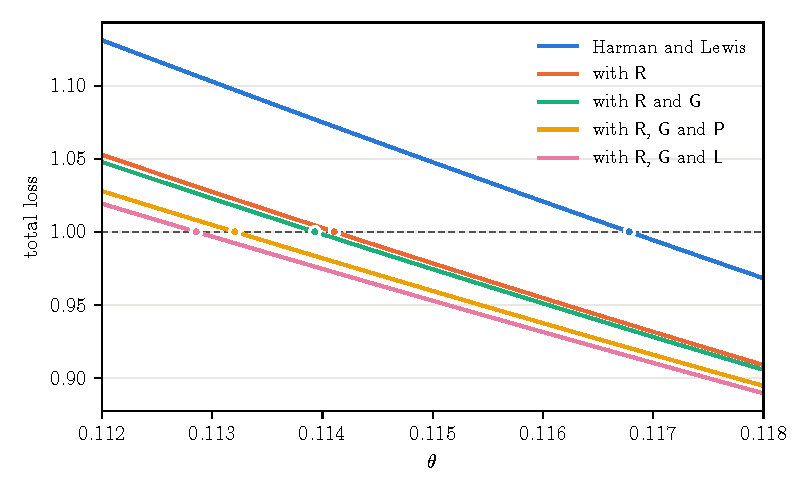
\includegraphics[width=0.8\textwidth]{../Code/figures/total_loss.pdf}
\caption{The total loss of each decomposition of Table~\ref{tab: roots}, computed by the first method of Section~\ref{sec: numerics} at $61$ values of $\theta$ from $0.112$ to $0.118$. The dashed line marks the total loss $1$, and the dots mark the values of $\theta$ in Table~\ref{tab: roots}.}
\label{fig: total loss}
\end{figure}

The computation is not carried out in interval arithmetic, so its accuracy is checked by refining the quadrature of the first method and by comparing the methods. For the first method, the losses at $\theta = 0.1129$ change by at most $2.5 \times 10^{-9}$, and their total by $2.6 \times 10^{-10}$, between the rule used for Table~\ref{tab: losses} and the finest rule tested, which has $512$ panels on the $\alpha$-axis for the regions $\mathsf{D}_k$, $32$ panels per axis for the regions $\mathsf{E}_k$, and $12$ nodes per subinterval. For $8$ coarser rules, with $12$ to $192$ nodes per axis, the total differs from that of the finest rule by amounts that decrease from $8.7 \times 10^{-6}$ to $6.8 \times 10^{-11}$ as the number of nodes grows. The totals of the methods differ by $1.2 \times 10^{-6}$, which is $1.1$ times the error estimate of the second method in Table~\ref{tab: losses}. Both quantities come almost entirely from $\mathsf{E}_{10}$. The gap $1 - \Phi(0.1129) = 9.97 \times 10^{-4}$ exceeds this difference, this error estimate and the change of the total under refinement by a factor of more than $800$.

\begin{proof}[Proof of Theorem~\ref{thm: sector}]
Let $\theta = 0.1129$. By Table~\ref{tab: losses}, $\Phi(\theta) < 1$, so Lemma~\ref{lem: lower bound} gives $S(\mathcal{A}, X^{1/2}) \gg XW^{-1}/\log X = X^{1/2 + \theta}/\log X$, uniformly in $\psi$. Since $S(\mathcal{A}, X^{1/2})$ is the number of Gaussian primes in $\mathcal{A}$, this is \eqref{eq: sector bound}.
\end{proof}

With the polytope $\mathsf{P}$ of \eqref{eq: polytope} in place of $\mathsf{L}$ (Section~\ref{subsec: groupings}), the first and second methods give $\Phi_{\mathsf{P}}(0.1133) = 0.9978243$ and $0.9978250$, so the same argument gives \eqref{eq: sector bound} with $\theta = 0.1133$, and hence $\{\sqrt{p}\} < p^{-0.2734}$ for infinitely many primes.

\section{Conclusion}
\label{sec: conclusion}

Of the total loss $0.999$ at $\theta = 0.1129$, the regions $\mathsf{D}_1$, $\mathsf{D}_2$ and $\mathsf{D}_4$ account for $0.877$. On these regions, after Buchstab's identity \eqref{eq: buchstab} introduces a third prime $r$ as in \eqref{eq: identity 35}, no factorization of $pqr$ satisfies the conditions \eqref{eq: linear exponents} of the linear estimate once $|r|^2$ is close to $|q|^2$. We have not found another grouping that gives the sums over these regions asymptotic formulas. A further improvement may need new arithmetic information for the Hecke characters $\lambda^m$ of Appendix~\ref{app: arithmetic}. \citet[p.~134]{harman2001gaussian} call the improvement of their arithmetic information ``the more interesting challenge''. The numerical evaluation of the losses could be made rigorous by interval arithmetic.

\section*{Data availability}

The code that computes every number in Section~\ref{sec: numerics} and Appendix~\ref{app: inequalities}, and the data of Figures~\ref{fig: domain} and~\ref{fig: total loss}, are in the folder \texttt{Code} of the repository \url{https://github.com/xuda-ye-math/Gaussian-Prime}. The code is written in Julia~1.13, and the file \texttt{Manifest.toml} of the folder fixes the versions of its packages. The file \texttt{README.md} of the folder describes each computation and its output.

\appendix

\section{Proofs of the linear and bilinear estimates}
\label{app: arithmetic}
\label{sec: arithmetic}

This appendix derives Lemmas~\ref{lem: type I} and~\ref{lem: type II} of Section~\ref{sec: estimates} from the arithmetic information. It begins with standard facts, which Sections~\ref{sec: decoupling}, \ref{sec: decomposition} and~\ref{sec: integrals} and Appendices~\ref{app: sieve} and~\ref{app: integrals} also use. Lemma~\ref{lem: prime ideal theorem} bounds sums over Gaussian primes, and Lemma~\ref{lem: counting} counts Gaussian integers and their divisors. Lemma~\ref{lem: perron} is the truncated Perron formula used in the proof of Lemma~\ref{lem: type II}.

\begin{lemma}
\label{lem: prime ideal theorem}
The number $\pi_G(y)$ of Gaussian primes of norm less than $y$ satisfies $\pi_G(y) = \mathrm{Li}(y) + \mathcal{O}(y \exp(-c (\log y)^{1/2}))$ for some $c > 0$, where $\mathrm{Li}(y) := \int_2^y dt/\log t$. Consequently, for fixed $B \Ge 0$ and $\kappa_0 \Ge 1$ and with $H := (\log X)^B$, the following hold once $X$ is large.
\begin{enumerate}[(a)]
\item If $Y \Ge \mu$ and $1 \Le \kappa \Le \kappa_0$, then
\begin{equation*}
\sum_{Y \Le |\varpi|^2 < Y(1 + 1/H)^{\kappa}} |\varpi|^{-2} \Le \frac{2\kappa}{H \log Y}.
\end{equation*}
\item $\sum_{|\varpi|^2 < y} |\varpi|^{-2} \Le \log\log y + C$ for $y \Ge 3$.
\item For fixed $a_0 > 0$, uniformly for $a_0 \Le a < b \Le 1$,
\begin{equation*}
\sum_{X^a \Le |\varpi|^2 < X^b} |\varpi|^{-2} = \log\frac{b}{a} + \mathcal{O}\Bigl( \frac{1}{\log X} \Bigr).
\end{equation*}
\item $\pi_G(y) - \pi_G(y/2) = (1 + \mathcal{O}(1/\log y))\, y/(2\log y)$.
\end{enumerate}
\end{lemma}

\begin{proof}
For $a \in \{1, 3\}$, let $\pi(y; 4, a)$ be the number of rational primes $\ell < y$ with $\ell \equiv a \pmod 4$. A Gaussian prime is $1 + i$, a prime of norm $\ell$ for a rational prime $\ell \equiv 1 \pmod 4$, or a rational prime $\ell \equiv 3 \pmod 4$, of norm $\ell^2$. Hence $\pi_G(y) = 2\pi(y; 4, 1) + \pi(y^{1/2}; 4, 3) + \mathcal{O}(1)$. The formula for $\pi_G(y)$ follows by partial summation from the prime number theorem in progressions modulo $4$ \citep[Section~1.2]{thorner2024refinements}, in the form
\begin{equation*}
\sum_{\ell \Le x,\ \ell \equiv a \,(4)} \log \ell = \frac{x}{2} \Bigl( 1 + \mathcal{O}\bigl( \exp(-c' (\log x)^{3/5} (\log\log x)^{-1/5}) \bigr) \Bigr), \qquad a \in \{1, 3\},
\end{equation*}
with a constant $c' > 0$. Statements (b), (c) and (d) follow by partial summation. In (a), the main term contributes $\log(1 + \kappa \log(1 + 1/H)/\log Y) \Le \kappa/(H \log Y)$, and the error term contributes $\mathcal{O}(\exp(-c (\log Y)^{1/2}))$. Since $\log Y \Ge (\log X)^{4/5}$, the error term is smaller than $1/(H \log Y)$ once $X$ is large, and (a) follows from $\kappa \Ge 1$.
\end{proof}

\begin{lemma}
\label{lem: counting}
\begin{enumerate}[(a)]
\item For $M \Ge 1$, the number of Gaussian integers $u$ with $X/(2M) \Le |u|^2 < X/M$ is at most $C X/M$. In particular $|\mathcal{B}_u| \Le C X/|u|^2$.
\item For $k \Ge 1$ and $Y \Ge 2$,
\begin{equation*}
\sum_{|n|^2 \Le Y} d(n)^k \ll_k Y (\log Y)^{2^k}, \qquad \sum_{|n|^2 \Le Y} d(n)^k |n|^{-2} \ll_k (\log Y)^{2^k}.
\end{equation*}
\item A Gaussian integer $n$ has at most $d(n)^{h - 1}$ ordered factorizations into $h$ factors.
\end{enumerate}
\end{lemma}

\begin{proof}
For (a), the count is $0$ if $X/M < 1$, and $\pi X/(8M) + \mathcal{O}((X/M)^{1/2} + 1)$ otherwise. For (b), $d$ is multiplicative with $d(\varpi^e) = e + 1$. So, by Lemma~\ref{lem: prime ideal theorem}(b), the sum of $d(n)^k |n|^{-2}$ is at most
\begin{equation*}
\prod_{|\varpi|^2 \Le Y} \sum_{e \Ge 0} (e + 1)^k |\varpi|^{-2e} \Le \exp\Bigl( \sum_{|\varpi|^2 \Le Y} \bigl( 2^k |\varpi|^{-2} + C_k |\varpi|^{-4} \bigr) \Bigr) \ll_k (\log Y)^{2^k},
\end{equation*}
and the sum of $d(n)^k$ is at most $Y$ times the sum of $d(n)^k |n|^{-2}$. For (c), the number $d_h(n)$ of ordered factorizations satisfies $d_h(n) = \sum_{u \mid n} d_{h-1}(n/u) \Le d(n)^{h-1}$, by induction on $h$.
\end{proof}

\begin{lemma}
\label{lem: perron}
For $y > 0$, $c > 0$ and $T_0 \Ge c$, let
\begin{equation*}
I(y) := \frac{1}{2\pi i} \int_{c - iT_0}^{c + iT_0} y^s\, \frac{ds}{s}.
\end{equation*} Then $|I(y)| \Le y^c \log(3T_0/c)$, and $|I(y) - \mathbf{1}[y > 1]| \Le y^c/(\pi T_0 |\log y|)$ for $y \neq 1$.
\end{lemma}

\begin{proof}
The bound $|I(y)| \Le y^c \log(3T_0/c)$ follows from $|I(y)| \Le (y^c/2\pi) \int_{-T_0}^{T_0} (c^2 + t^2)^{-1/2}\, dt$. For $y > 1$, move the segment to $\mathrm{Re}\, s = -K$ and let $K \to \infty$. The residue at $0$ is $1$, the integral over $\mathrm{Re}\, s = -K$ tends to $0$, and each horizontal side is at most
\begin{equation*}
\frac{1}{2\pi T_0} \int_{-\infty}^{c} y^u\, du = \frac{y^c}{2\pi T_0 \log y}.
\end{equation*}
For $y < 1$, move the segment to $\mathrm{Re}\, s = K$, where there is no pole, and obtain the same bound with $|\log y|$.
\end{proof}

For an integer $m$ and a Gaussian integer $n \neq 0$ put $\lambda^m(n) := (n/|n|)^{4m}$, as in \citet[p.~122]{harman2001gaussian}. This is a Hecke character. It is unchanged when $n$ is multiplied by a unit, so it is completely multiplicative under the identification of associates fixed in Section~\ref{sec: introduction}. Since $\lambda^m(n) = e^{4im \arg n}$, it detects the argument of $n$ modulo $\pi/2$. Lemmas~\ref{lem: sector inequality} to~\ref{lem: type I input} below are quoted without proof from \citet{harman2001gaussian}, and Lemma~\ref{lem: type I input} combines their Lemmas~6 and~7. Lemmas~\ref{lem: sector inequality} and~\ref{lem: type I input} give the linear estimate, Lemma~\ref{lem: type I}. Lemmas~\ref{lem: sector inequality}, \ref{lem: mean value} and~\ref{lem: hecke pnt} give the bilinear estimate, Lemma~\ref{lem: type II}.

\begin{lemma}[\citet{harman2001gaussian}, (12)]
\label{lem: sector inequality}
For every $T \Ge 1$ and all non-negative weights $a_n$,
\begin{equation*}
\sum_{n \in \mathcal{A}} a_n = \frac{2}{\pi W} \sum_{n \in \mathcal{B}} a_n + \mathcal{O}\Bigl( \frac{1}{T} \sum_{n \in \mathcal{B}} a_n \Bigr) + \mathcal{O}\Bigl( \frac{1}{W} \sum_{m = 1}^{T} \Bigl| \sum_{n \in \mathcal{B}} a_n \lambda^m(n) \Bigr| \Bigr).
\end{equation*}
\end{lemma}

Harman and Lewis state Lemma~\ref{lem: sector inequality} for any weights and note that it follows from \citet[Chapter~2]{baker1986diophantine}. It is quoted here for non-negative weights, the only ones used.

\begin{lemma}[\citet{harman2001gaussian}, Lemma~1]
\label{lem: mean value}
For $T \Ge 1$, $N \Ge 1$ and all coefficients $c(n)$,
\begin{equation*}
\sum_{m = 1}^{T} \Bigl| \sum_{|n|^2 \Le N} c(n) \lambda^m(n) \Bigr|^2 \ll (T + N) \sideset{}{'}\sum_{|n|^2 \Le N} |c_1(n)|^2, \qquad c_1(n) := \sum_{\arg u = \arg n} c(u),
\end{equation*}
where $\sum'$ runs over the primitive Gaussian integers $n = x + iy$, $\gcd(x, y) = 1$.
\end{lemma}

\begin{lemma}[\citet{harman2001gaussian}, Lemma~4]
\label{lem: hecke pnt}
Let $R, T_0 \Ge 2$, $T \Ge S \Ge R + \exp((\log T T_0)^{4/5})$, $1 \Le m \Le T$ and $|t| \Le T_0$. Then
\begin{equation*}
\Bigl| \sum_{R \Le |\varpi|^2 < S} |\varpi|^{2it} \lambda^m(\varpi) \Bigr| \ll S \exp\Bigl( -\frac{\log S}{2 (\log T T_0)^{7/10}} \Bigr).
\end{equation*}
\end{lemma}

Lemma~\ref{lem: mean value} is \citet[Lemma~6]{coleman1993rosser}, and Lemma~\ref{lem: hecke pnt} rests on the zero-free region of \citet{coleman1990zero}.

\begin{lemma}[\citet{harman2001gaussian}, Lemmas~6 and~7]
\label{lem: type I input}
Let $A > 0$, $T := W (\log X)^A$, and let $a_u$, $b_v$ be divisor-bounded.
\begin{enumerate}[(a)]
\item If $U \Le X^{\tau} \mu^{-1}$, then
\begin{equation*}
\sum_{m = 1}^{T} \Bigl| \sum_{u \sim U} a_u \sum_{ut \in \mathcal{B}} \lambda^m(ut) \Bigr| \ll X (\log X)^{-A}.
\end{equation*}
\item If $U \Le X^{\zeta} \mu^{-1}$, $V \Le X^{\rho} \mu^{-1}$ and $UV \Le X^{\nu} \mu^{-1}$, then
\begin{equation*}
\sum_{m = 1}^{T} \Bigl| \sum_{u \sim U} a_u \sum_{v \sim V} b_v \sum_{uvt \in \mathcal{B}} \lambda^m(uvt) \Bigr| \ll X (\log X)^{-A}.
\end{equation*}
\end{enumerate}
Here $t$ runs over all Gaussian integers with the stated product in $\mathcal{B}$.
\end{lemma}

Remark~\ref{rem: annulus} in Appendix~\ref{app: comparison} explains the conditions $ut \in \mathcal{B}$ and $uvt \in \mathcal{B}$ of Lemma~\ref{lem: type I input}.

\begin{proof}[Proof of Lemma~\ref{lem: type I}]
With $c'_n := \sum_{v \mid n} c_v \Ge 0$,
\begin{equation*}
\sum_v c_v |\mathcal{A}_v| = \sum_{n \in \mathcal{A}} c'_n, \qquad \sum_{n \in \mathcal{B}} c'_n = \sum_v c_v |\mathcal{B}_v|.
\end{equation*}
Apply Lemma~\ref{lem: sector inequality} with $a_n = c'_n$ and $T = W (\log X)^A$. By Lemma~\ref{lem: counting}, its error term $\mathcal{O}(T^{-1} \sum_{n \in \mathcal{B}} c'_n)$ is at most
\begin{equation*}
W^{-1} (\log X)^{-A} \cdot C X \sum_v c_v |v|^{-2} \ll X W^{-1} (\log X)^{C - A}.
\end{equation*} Its error term with the sums over $\lambda^m$ is
\begin{equation*}
\frac{1}{W} \sum_{m \Le T} \Bigl| \sum_v c_v \sum_{vt \in \mathcal{B}} \lambda^m(vt) \Bigr|.
\end{equation*} Under (a), after the range of $v$ is split into $\mathcal{O}(\log X)$ dyadic ranges, it is $\ll X W^{-1} (\log X)^{1 - A}$ by Lemma~\ref{lem: type I input}(a). Under (b) it is $\ll X W^{-1} (\log X)^{-A}$ by Lemma~\ref{lem: type I input}(b). Since $A$ is arbitrary, the lemma follows.
\end{proof}

\begin{proof}[Proof of Lemma~\ref{lem: type II}]
Lemma~\ref{lem: perron} separates the variables $u$, $v$ and $\varpi$. Cauchy's inequality and Lemma~\ref{lem: mean value} then bound the sums over $u$ and over $v$ in mean square over $m$, and Lemma~\ref{lem: hecke pnt} bounds the sum over $\varpi$ uniformly in $m$.

Fix $A$, put $T := W (\log X)^A$, and let $E_m$ be the sum of $a_u b_v \lambda^m(uv\varpi)$ over the triples counted in \eqref{eq: type II} with $\mathcal{E} = \mathcal{B}$. As in the proof of Lemma~\ref{lem: type I}, it suffices to show that $\sum_{m \Le T} |E_m| \ll X (\log X)^{-A}$. A triple occurs only if $X/(8UV) \Le |\varpi|^2 < X/(UV)$. Put $Z_1' := \max(Z_1, X/(8UV))$ and $Z_2' := \min(Z_2, X/(UV))$, and assume that $Z_1' < Z_2'$, since otherwise $E_m = 0$. For $N = |uv\varpi|^2 \Le 4X$, write $\mathbf{1}[X/2 \Le N < X] = \mathbf{1}[X/N > 1] - \mathbf{1}[(X/2)/N > 1]$, and apply Lemma~\ref{lem: perron} to $y = Y/N$ for $Y \in \{X, X/2\}$, with $c = 1/\log X$ and $T_0 = X^3$. If $|N - Y| \Ge 1/2$, then $|\log y| \Ge 1/(16X)$ and the error is at most $16eX/(\pi T_0)$. At most $2$ integers $N$ have $|N - Y| < 1/2$, and for them we use $|I(y)| \Le e \log(3T_0/c)$. Each $N \Le 4X$ is the norm of $X^{o(1)}$ Gaussian integers, and by Lemma~\ref{lem: counting}(c) each of these is the product of $X^{o(1)}$ triples, each with weight $a_u b_v \Le X^{o(1)}$. Since $\lambda^m$ is completely multiplicative, this gives
\begin{equation}
\label{eq: perron type II}
E_m = \frac{1}{2\pi i} \int_{c - iT_0}^{c + iT_0} \bigl(X^s - (X/2)^s\bigr) F_m(s) G_m(s) \mathfrak{p}_m(s)\, \frac{ds}{s} + \mathcal{O}(X^{o(1)}),
\end{equation}
where
\begin{equation*}
F_m(s) := \sum_{u \sim U} a_u \lambda^m(u) |u|^{-2s}, \qquad G_m(s) := \sum_{v \sim V} b_v \lambda^m(v) |v|^{-2s}, \qquad \mathfrak{p}_m(s) := \sum_{Z_1' \Le |\varpi|^2 < Z_2'} \lambda^m(\varpi) |\varpi|^{-2s}.
\end{equation*} Since $|X^s| = e$ and $\int_{-T_0}^{T_0} |c + it|^{-1}\, dt \ll \log X$, summing \eqref{eq: perron type II} over $m \Le T$ gives
\begin{equation}
\label{eq: type II reduction}
\sum_{m \Le T} |E_m| \ll \log X \cdot \sup_{|t| \Le T_0} \sum_{m \Le T} \bigl| F_m G_m \mathfrak{p}_m \bigr|(c + it) + X^{\sigma + o(1)}.
\end{equation}
By Cauchy's inequality, the sum over $m$ in \eqref{eq: type II reduction} satisfies
\begin{equation*}
\sum_{m \Le T} \bigl| F_m G_m \mathfrak{p}_m \bigr|(c + it) \Le \max_{m \Le T} |\mathfrak{p}_m(c + it)| \Bigl( \sum_{m \Le T} |F_m(c + it)|^2 \Bigr)^{1/2} \Bigl( \sum_{m \Le T} |G_m(c + it)|^2 \Bigr)^{1/2}.
\end{equation*}

To bound $\sum_m |F_m|^2$, apply Lemma~\ref{lem: mean value} with $2U$ in place of $N$ and with $c(u) = a_u |u|^{-2s}$ for $u \sim U$. A Gaussian integer $u$ with $\arg u = \arg n$, $n$ primitive, is $u = kn$ with $k$ a positive rational integer. So $|c_1(n)| \Le \sum_k d(kn)^{C_0}$, where $k \Ge 1$ runs over the integers with $k^2 |n|^2 \in [U, 2U)$. This sum has at most $(2U)^{1/2}/|n|$ terms. By Cauchy's inequality and $d(kn) \Le d(k) d(n)$,
\begin{equation}
\label{eq: c1 bound}
\sideset{}{'}\sum_{n} |c_1(n)|^2 \Le (2U)^{1/2} \sum_{k^2 \Le 2U} d(k)^{2C_0} \sum_{|n|^2 < 2U/k^2} d(n)^{2C_0} |n|^{-1}.
\end{equation}
By Lemma~\ref{lem: counting}(b) and partial summation, the sum of $d(n)^{2C_0} |n|^{-1}$ in \eqref{eq: c1 bound} is $\ll (U/k^2)^{1/2} (\log X)^C$. The remaining sum, of $d(k)^{2C_0}/k$ over the rational integers $k \Le (2U)^{1/2}$, is at most a product over the rational primes $\ell \Le (2U)^{1/2}$:
\begin{equation*}
\prod_{\ell \Le (2U)^{1/2}} \sum_{e \Ge 0} (e + 1)^{4C_0} \ell^{-e} \ll (\log X)^{2^{4C_0}}.
\end{equation*} Here $d(\ell^e) \Le (e + 1)^2$ for every rational prime $\ell$, and $\sum_{\ell \Le x} 1/\ell \Le \log\log x + \mathcal{O}(1)$ follows from the prime number theorem modulo $4$. So the right side of \eqref{eq: c1 bound} is $\ll U (\log X)^C$, and, since $T \Le C_1 U (\log X)^A$,
\begin{equation*}
\sum_{m \Le T} |F_m|^2 \ll (T + U) U (\log X)^C \ll U^2 (\log X)^{A + C}.
\end{equation*}
The same bound holds for $G_m$ with $V$ in place of $U$.

It remains to bound $\mathfrak{p}_m(c + it)$. The weight $|\varpi|^{-2c}$ in its terms is decreasing in $|\varpi|^2$ and lies in $[e^{-2}, 1]$. By partial summation, $|\mathfrak{p}_m(c + it)|$ is at most $2$ times the largest value, over $Z \in [Z_1', Z_2']$, of
\begin{equation*}
\Bigl| \sum_{Z_1' \Le |\varpi|^2 < Z} \lambda^m(\varpi) |\varpi|^{-2it} \Bigr|.
\end{equation*}
Each of these sums is the difference of the sums over $2 \Le |\varpi|^2 < S$ for $S = Z$ and for $S = Z_1'$. Lemma~\ref{lem: hecke pnt} applies to them with $R = 2$, $|t| \Le T_0$ and $1 \Le m \Le T$, once $T \Ge S \Ge 2 + \exp((\log T T_0)^{4/5})$. The condition $S \Le T$ holds, since $\theta < 1/6$ gives $S \Le X/(UV) \Le C_1^2 X^{2\theta} \Le T$. For the lower condition on $S$, $\log(T T_0) \Le 4 \log X$ and $4^{4/5} < 3.1$ give
\begin{equation*}
S \Ge \frac{\mu^4}{2} > 2 + \exp\bigl( (\log T T_0)^{4/5} \bigr).
\end{equation*}
Since $S \exp(-\log S/(2(\log T T_0)^{7/10}))$ increases with $S$ and $\log Z_2' \Ge \log(\mu^4/2)$, Lemma~\ref{lem: hecke pnt} gives
\begin{equation*}
\max_m |\mathfrak{p}_m| \ll \frac{X}{UV} \exp\Bigl( -\frac34 (\log X)^{1/10} \Bigr).
\end{equation*}
Collecting the bounds in \eqref{eq: type II reduction}, we obtain
\begin{equation*}
\sum_{m \Le T} |E_m| \ll X (\log X)^{A + C + 1} \exp\Bigl( -\frac34 (\log X)^{1/10} \Bigr) + X^{\sigma + o(1)} \ll X (\log X)^{-A}.
\end{equation*}
\end{proof}

\section{Proofs of the sieve lemmas}
\label{app: sieve}

This appendix proves Lemmas~\ref{lem: fundamental}, \ref{lem: level large} and~\ref{lem: level small} of Section~\ref{sec: estimates} and Lemma~\ref{lem: decoupling} of Section~\ref{sec: decoupling}. In the proofs of Lemmas~\ref{lem: level large} and~\ref{lem: level small}, Lemma~\ref{lem: fundamental} treats the sifting by the primes of norm below $\mu^4$, and Lemma~\ref{lem: type II} is applied only to primes of norm at least $\mu^4/2$. As in Section~\ref{sec: decoupling}, short intervals remove the conditions that couple the variables.

\begin{proof}[Proof of Lemma~\ref{lem: fundamental}]
The proof is Brun's pure sieve: the inclusion--exclusion over the primes of norm below $z_0(u)$ that divide the cofactor is truncated after the divisors with $M$ prime factors, and the divisors with $M + 1$ prime factors bound the error of the truncation. Put $M + 1 := \lfloor (\varepsilon_0/4) (\log X)^{1/5} \rfloor$. For $z \Ge 1$, let $\mathfrak{P}(z)$ be the product of the primes of norm less than $z$, and for a squarefree $\mathfrak{d}$ let $\mathfrak{o}(\mathfrak{d})$ be its number of prime factors. For squarefree $\mathfrak{d}$ put
\begin{equation*}
\mathfrak{b}^{\pm}_{\mathfrak{d}}(u) := \mathbf{1}\bigl[\mathfrak{d} \mid \mathfrak{P}(z_0(u)),\ \mathfrak{o}(\mathfrak{d}) \Le M,\ (-1)^{\mathfrak{o}(\mathfrak{d})} = \pm 1\bigr], \qquad \mathfrak{b}^{0}_{\mathfrak{d}}(u) := \mathbf{1}\bigl[\mathfrak{d} \mid \mathfrak{P}(z_0(u)),\ \mathfrak{o}(\mathfrak{d}) = M + 1\bigr],
\end{equation*}
and let $\mathfrak{b}^{+}_{\mathfrak{d}}(u)$, $\mathfrak{b}^{-}_{\mathfrak{d}}(u)$ and $\mathfrak{b}^{0}_{\mathfrak{d}}(u)$ be $0$ for $\mathfrak{d}$ not squarefree. We first show that $\sum_u c_u S'(\mathcal{E}_u, z_0(u))$ has an asymptotic formula if, for each $\mathfrak{b} \in \{\mathfrak{b}^+, \mathfrak{b}^-, \mathfrak{b}^0\}$, the sum $\sum_{u, \mathfrak{d}} c_u \mathfrak{b}_{\mathfrak{d}}(u) |\mathcal{E}_{u\mathfrak{d}}|$ has one.

For $u \mid n$, let $\mathfrak{n}$ be the number of distinct primes of norm less than $z_0(u)$ that divide $n/u$. The number of $\mathfrak{d} \mid \mathfrak{P}(z_0(u))$ with $\mathfrak{d} \mid n/u$ and $\mathfrak{o}(\mathfrak{d}) = i$ is $\binom{\mathfrak{n}}{i}$. For $\mathfrak{n} \Ge 1$,
\begin{equation*}
\sum_{i=0}^{M} (-1)^i \binom{\mathfrak{n}}{i} = (-1)^M \binom{\mathfrak{n} - 1}{M},
\end{equation*}
and this is at most $\binom{\mathfrak{n}}{M+1}$ in absolute value. Hence
\begin{equation}
\label{eq: bonferroni}
S'(\mathcal{E}_u, z_0(u)) = \sum_{\mathfrak{d}} \bigl( \mathfrak{b}^+_{\mathfrak{d}}(u) - \mathfrak{b}^-_{\mathfrak{d}}(u) \bigr) |\mathcal{E}_{u\mathfrak{d}}| + \Delta_u, \qquad |\Delta_u| \Le \sum_{\mathfrak{d}} \mathfrak{b}^0_{\mathfrak{d}}(u) |\mathcal{E}_{u\mathfrak{d}}|.
\end{equation}
Multiply by $c_u$ and sum over $u$. By assumption, the sums of $c_u (\mathfrak{b}^+_{\mathfrak{d}}(u) - \mathfrak{b}^-_{\mathfrak{d}}(u)) |\mathcal{A}_{u\mathfrak{d}}|$ in \eqref{eq: bonferroni} over $u$ and $\mathfrak{d}$ are $2/(\pi W)$ times those for $\mathcal{B}$, up to $\mathcal{O}(XW^{-1}(\log X)^{-A})$. The remainders $\Delta_u$ contribute at most
\begin{equation*}
\sum_{u, \mathfrak{d}} c_u \mathfrak{b}^0_{\mathfrak{d}}(u) \Bigl( |\mathcal{A}_{u\mathfrak{d}}| + \frac{2}{\pi W} |\mathcal{B}_{u\mathfrak{d}}| \Bigr) = \frac{4}{\pi W} \sum_{u, \mathfrak{d}} c_u \mathfrak{b}^0_{\mathfrak{d}}(u) |\mathcal{B}_{u\mathfrak{d}}| + \mathcal{O}\bigl(XW^{-1}(\log X)^{-A}\bigr),
\end{equation*}
where the equality holds by assumption. By Lemma~\ref{lem: counting} and Lemma~\ref{lem: prime ideal theorem}(b), with $\sum_{|\varpi|^2 < \mu^4} |\varpi|^{-2} \Le \log\log X$,
\begin{equation*}
\sum_{u, \mathfrak{d}} c_u \mathfrak{b}^0_{\mathfrak{d}}(u) |\mathcal{B}_{u\mathfrak{d}}| \Le C X \sum_u c_u |u|^{-2} \frac{(\log\log X)^{M+1}}{(M+1)!} \ll X (\log X)^C \Bigl( \frac{e \log\log X}{M + 1} \Bigr)^{M+1} \Le X (\log X)^C e^{-(M+1)},
\end{equation*}
once $M + 1 \Ge e^2 \log\log X$. Finally $e^{-(M+1)} \Le \exp(-(\varepsilon_0/5)(\log X)^{1/5})$ is smaller than every power of $1/\log X$.

It remains to show that the assumption holds in cases (a) and (b). The indicators $\mathfrak{b}_{\mathfrak{d}}(u)$ vanish unless $|\mathfrak{d}|^2 < \mu^{4(M+1)} \Le X^{\varepsilon_0}$. In case (a), $\sum_{v = u\mathfrak{d}} c_u \mathfrak{b}_{\mathfrak{d}}(u)$ is non-negative, at most $d(v)^{C_0 + 1}$, and supported on $|v|^2 \Le X^{\tau} \mu^{-1}$, so Lemma~\ref{lem: type I}(a) applies. In case (b), $\mathfrak{b}_{\mathfrak{d}}$ does not depend on $u$, since $z_0$ is constant. After the range of $u_2 \mathfrak{d}$ is split into dyadic ranges, Lemma~\ref{lem: type I}(b) applies with $u_2 \mathfrak{d}$ as its variable $u'$.
\end{proof}

The proofs of Lemmas~\ref{lem: level large} and~\ref{lem: level small} confine primes to the short intervals $J_\lambda$ of Section~\ref{sec: decoupling}, with the indices $\lambda_q$ defined there. The following estimates bound the terms in which two primes share a short interval. For an index $\lambda$ put $\mathfrak{s}_\lambda := \sum_{|\varpi|^2 \in J_\lambda} |\varpi|^{-2}$. If $\xi_{\lambda + 1} > \mu^4$, then $\xi_\lambda \Ge \mu^4/2 \Ge \mu$, so Lemma~\ref{lem: prime ideal theorem}(a) gives
\begin{equation}
\label{eq: short interval mass}
\mathfrak{s}_\lambda \Le \frac{2}{H \log(\mu^4/2)}.
\end{equation}
In sums over $\lambda$, the index runs over the $\lambda$ with $J_\lambda \cap [1, 2X] \neq \emptyset$. By Lemma~\ref{lem: prime ideal theorem}(b), $\sum_\lambda \mathfrak{s}_\lambda \Le 2\log\log X$, so that
\begin{equation}
\label{eq: short interval square}
\sum_{\lambda:\ \xi_{\lambda + 1} > \mu^4} \mathfrak{s}_\lambda^2 \Le \frac{4 \log\log X}{H \log(\mu^4/2)}.
\end{equation}

\begin{proof}[Proof of Lemma~\ref{lem: level large}]
Buchstab's identity \eqref{eq: buchstab} lowers the level $l(n)$ to $\mu^4$, where Lemma~\ref{lem: fundamental} applies. Once the prime $q$ of the subtracted sum is confined to a short interval, that sum takes the form \eqref{eq: type II}, up to terms that \eqref{eq: short interval mass} and \eqref{eq: short interval square} make small. Fix $A$, let $C$ be such that $\sum_{|n|^2 \Le X} a_n |n|^{-2} \Le (\log X)^C$ (Lemma~\ref{lem: counting}), and take $B = A + C + 3$. Split the support of $a$ into $\mathcal{N}_1 := \{n : l(n) \Le \mu^4\}$ and $\mathcal{N}_2 := \{n : l(n) > \mu^4\}$. On $\mathcal{N}_1$, Lemma~\ref{lem: fundamental}(a) applies with $c_n = a_n \mathbf{1}_{\mathcal{N}_1}(n)$, the level $z_0 = l$ and $\varepsilon_0 = \varepsilon/2$, since $X^{\tau - \varepsilon} \Le X^{\tau - \varepsilon/2} \mu^{-1}$. On $\mathcal{N}_2$, Buchstab's identity \eqref{eq: buchstab} gives
\begin{equation}
\label{eq: buchstab at mu4}
S'(\mathcal{E}_n, l(n)) = S'(\mathcal{E}_n, \mu^4) - \sum_{\mu^4 \Le |q|^2 < l(n)} S'(\mathcal{E}_{nq}, q),
\end{equation}
and the term $S'(\mathcal{E}_n, \mu^4)$ of \eqref{eq: buchstab at mu4}, summed with $a_n$, has an asymptotic formula by Lemma~\ref{lem: fundamental}(a) at the constant level $\mu^4$. It remains to treat
\begin{equation*}
\Sigma_0(\mathcal{E}) := \sum_{n \in \mathcal{N}_2} a_n \sum_{\mu^4 \Le |q|^2 < l(n)} S'(\mathcal{E}_{nq}, q).
\end{equation*}

Two conditions couple $n$, $q$ and the cofactor: $|q|^2 < l(n)$, and the condition that every prime factor of the cofactor is $\succcurlyeq q$. For $n \in \mathcal{N}_2$ let $\lambda(n)$ be the index with $l(n) \in J_{\lambda(n)}$. Then
\begin{equation*}
\mathbf{1}[|q|^2 < l(n)] = \mathbf{1}[\lambda_q < \lambda(n)] + \mathbf{1}[\lambda_q = \lambda(n)]\, \mathbf{1}[|q|^2 < l(n)].
\end{equation*} Moreover, a prime factor $\varpi' \prec q$ of the cofactor with norm at least $\xi_{\lambda_q}$ has its norm in $J_{\lambda_q}$, so
\begin{equation*}
0 \Le S'(\mathcal{E}_{nq}, \xi_{\lambda_q}) - S'(\mathcal{E}_{nq}, q) \Le \sum_{|\varpi'|^2 \in J_{\lambda_q}} |\mathcal{E}_{nq\varpi'}|.
\end{equation*} With $q$ running over the primes of norm at least $\mu^4$ in $J_\lambda$, this gives
\begin{equation}
\label{eq: level large split}
\Bigl| \Sigma_0(\mathcal{E}) - \sum_\lambda \mathfrak{M}_\lambda(\mathcal{E}) \Bigr| \Le \sum_\lambda \bigl( \mathfrak{D}_\lambda(\mathcal{E}) + \mathfrak{D}'_\lambda(\mathcal{E}) \bigr),
\end{equation}
where
\begin{equation*}
\mathfrak{M}_\lambda(\mathcal{E}) := \sum_{\lambda(n) > \lambda} a_n \sum_q S'(\mathcal{E}_{nq}, \xi_\lambda), \quad \mathfrak{D}_\lambda(\mathcal{E}) := \sum_{\lambda(n) = \lambda} a_n \sum_q |\mathcal{E}_{nq}|, \quad \mathfrak{D}'_\lambda(\mathcal{E}) := \sum_{\lambda(n) \Ge \lambda} a_n \sum_q \sum_{|\varpi'|^2 \in J_\lambda} |\mathcal{E}_{nq\varpi'}|.
\end{equation*}
Each of these sums has the form
\begin{equation*}
\sum_{u, v} b'_u b_v\, \#\{q : |q|^2 \in J_\lambda,\ |q|^2 \Ge \mu^4,\ uvq \in \mathcal{E}\},
\end{equation*}
with $u = n$, with $b'_u$ equal to $a_n$ restricted to $\lambda(n) > \lambda$, $\lambda(n) = \lambda$ or $\lambda(n) \Ge \lambda$, and with $v$ the cofactor of $nq$. For $\mathfrak{M}_\lambda$, the coefficient $b_v$ is the indicator that every prime factor of $v$ has norm at least $\xi_\lambda$. For $\mathfrak{D}_\lambda$ it is $1$, and for $\mathfrak{D}'_\lambda$ it is the number of primes in $J_\lambda$ dividing $v$, which is at most $d(v)$. For $\lambda(n) \Ge \lambda$ and $|q|^2 \in J_\lambda$,
\begin{equation*}
|q|^2 < \xi_{\lambda+1} \Le (1 + 1/H)\, l(n) \Le \frac{2C_l X^{\tau}}{|n|^2},
\end{equation*}
so $|v|^2 \Ge (X/2)/|nq|^2 \Ge W/(4C_l)$. In addition, $|n|^2 \Ge W/C_l$ and $|q|^2 \Ge \mu^4$. After $u$ and $v$ are split into dyadic ranges, Lemma~\ref{lem: type II} gives $\mathfrak{M}_\lambda$, $\mathfrak{D}_\lambda$ and $\mathfrak{D}'_\lambda$ asymptotic formulas, uniformly in $\lambda$. At most $2H \log X$ indices and $\mathcal{O}((\log X)^2)$ pairs of dyadic ranges occur, so Lemma~\ref{lem: type II} is applied $\mathcal{O}(H (\log X)^3)$ times. With the saving $(\log X)^{-A-B-5}$ in each application, the errors add up to $\mathcal{O}(XW^{-1}(\log X)^{-A})$.

By \eqref{eq: level large split}, $\Sigma_0(\mathcal{A}) - \frac{2}{\pi W} \Sigma_0(\mathcal{B})$ is $\mathcal{O}(XW^{-1}(\log X)^{-A})$ plus
\begin{equation*}
\mathcal{O}\Bigl( \sum_\lambda (\mathfrak{D}_\lambda + \mathfrak{D}'_\lambda)(\mathcal{A}) + \frac{2}{\pi W} \sum_\lambda (\mathfrak{D}_\lambda + \mathfrak{D}'_\lambda)(\mathcal{B}) \Bigr),
\end{equation*}
and the sums over $\mathcal{A}$ equal $\frac{2}{\pi W}$ times those over $\mathcal{B}$ up to the same error. By Lemma~\ref{lem: counting},
\begin{equation*}
\sum_\lambda \mathfrak{D}_\lambda(\mathcal{B}) \Le C X \sum_n a_n |n|^{-2} \mathfrak{s}_{\lambda(n)}, \qquad \sum_\lambda \mathfrak{D}'_\lambda(\mathcal{B}) \Le C X \sum_n a_n |n|^{-2} \sum_\lambda \mathfrak{s}_\lambda^2,
\end{equation*}
and, by \eqref{eq: short interval mass} and \eqref{eq: short interval square}, both are $\ll X (\log X)^C \log\log X/(H (\log X)^{4/5}) \ll X (\log X)^{-A}$. Hence $\Sigma_0$ has an asymptotic formula, and so does $\sum_n a_n S'(\mathcal{E}_n, l(n))$.
\end{proof}

\begin{proof}[Proof of Lemma~\ref{lem: level small}]
Here $|n|^2$ may be much smaller than $W$, while Lemma~\ref{lem: level large} needs $|n|^2 \Ge W/C_l$. So Buchstab's identity \eqref{eq: buchstab} is iterated until the product of $n$ and the primes it introduces has norm at least $W$, and Lemma~\ref{lem: level large} is applied to that product. Fix $A$, let $C$ be as in the proof of Lemma~\ref{lem: level large}, and take $B = A + C + 4$. The set $\mathcal{N}_1 := \{n : l(n) \Le \mu^4\}$ is handled by Lemma~\ref{lem: fundamental}(a) with the level $l$, since $|n|^2 < W \Le X^{\tau - 2\theta}$. On $\mathcal{N}_2 := \{n : l(n) > \mu^4\}$, \eqref{eq: buchstab at mu4} holds, and the term $S'(\mathcal{E}_n, \mu^4)$ of \eqref{eq: buchstab at mu4} again has an asymptotic formula by Lemma~\ref{lem: fundamental}(a). It remains to treat the sum $\Sigma_0(\mathcal{E})$, defined as in the proof of Lemma~\ref{lem: level large}.

A \emph{chain of length} $i \Ge 0$ is a tuple $\mathfrak{c} = (n, p_1, \dots, p_i, q)$ with $n \in \mathcal{N}_2$ and primes $p_1 \succ \dots \succ p_i \succ q$ of norm at least $\mu^4$, such that the largest of these primes ($p_1$, or $q$ if $i = 0$) has norm less than $l(n)$, and $|n p_1 \cdots p_{i'}|^2 < W$ for $1 \Le i' \Le i$. Write $N(\mathfrak{c}) := n p_1 \cdots p_i q$ and $q(\mathfrak{c}) := q$. Let $\mathcal{K}_i$ be the set of chains of length $i$, split into the exits $\mathcal{K}^{\Ge}_i$, with $|N(\mathfrak{c})|^2 \Ge W$, and the continuations $\mathcal{K}^{<}_i$, with $|N(\mathfrak{c})|^2 < W$, and put
\begin{equation*}
\Sigma_i(\mathcal{E}) := \sum_{\mathfrak{c} \in \mathcal{K}_i} a_n S'(\mathcal{E}_{N(\mathfrak{c})}, q(\mathfrak{c})).
\end{equation*}
For $\mathfrak{c} \in \mathcal{K}^{<}_i$, Buchstab's identity \eqref{eq: buchstab} gives
\begin{equation*}
S'(\mathcal{E}_{N(\mathfrak{c})}, q) = S'(\mathcal{E}_{N(\mathfrak{c})}, \mu^4) - \sum_{q' \prec q,\ |q'|^2 \Ge \mu^4} S'(\mathcal{E}_{N(\mathfrak{c}) q'}, q').
\end{equation*}
The map $(\mathfrak{c}, q') \mapsto (n, p_1, \dots, p_i, q, q')$, on the pairs that occur in these sums, is a bijection onto $\mathcal{K}_{i+1}$. Hence $\Sigma_i = \mathfrak{E}_i + \mathfrak{F}_i - \Sigma_{i+1}$, where
\begin{equation*}
\mathfrak{E}_i(\mathcal{E}) := \sum_{\mathfrak{c} \in \mathcal{K}^{\Ge}_i} a_n S'(\mathcal{E}_{N(\mathfrak{c})}, q(\mathfrak{c})), \qquad \mathfrak{F}_i(\mathcal{E}) := \sum_{\mathfrak{c} \in \mathcal{K}^{<}_i} a_n S'(\mathcal{E}_{N(\mathfrak{c})}, \mu^4).
\end{equation*}
A chain of length $i$ has $\mu^{4i} \Le |p_1 \cdots p_i|^2 < W$, so $\mathcal{K}_i$ is empty for $i > i_{\max} := \lfloor \sigma (\log X)^{1/5}/4 \rfloor$. Hence, for $\mathcal{E} = \mathcal{A}$ and for $\mathcal{E} = \mathcal{B}$,
\begin{equation}
\label{eq: chain sum}
\Sigma_0 = \sum_{i=0}^{i_{\max}} (-1)^i (\mathfrak{E}_i + \mathfrak{F}_i).
\end{equation}

The primes of a chain are distinct and their order is forced, so a chain is determined by its product and the set of its primes. The number of chains with a given product $N$ is therefore at most $d(N)$, and every coefficient defined from chains in this proof is at most $d(N)^{C_0 + 1}$, uniformly in $i$. The sum $\mathfrak{F}_i$ is $\sum_N c_i(N) S'(\mathcal{E}_N, \mu^4)$, where $c_i(N)$ is the sum of $a_n$ over the chains $\mathfrak{c} \in \mathcal{K}^{<}_i$ with $N(\mathfrak{c}) = N$. This $c_i(N)$ is supported on $|N|^2 < W$, so Lemma~\ref{lem: fundamental}(a) gives $\mathfrak{F}_i$ an asymptotic formula, uniformly in $i$.

For the exits, Lemma~\ref{lem: level large} is applied with $N(\mathfrak{c})$ in place of $n$, and \eqref{eq: exit bound} below gives its hypotheses. Let $j_{\max} := \lceil \sigma/\theta \rceil$ and $C_E := 2 C_l^{j_{\max} + 2}$. We claim that every $\mathfrak{c} \in \mathcal{K}^{\Ge}_i$ satisfies
\begin{equation}
\label{eq: exit bound}
W \Le |N(\mathfrak{c})|^2 \Le C_E X^{\tau - \theta/2}, \qquad |N(\mathfrak{c})|^2 |q(\mathfrak{c})|^2 \Le C_E X^{\tau}.
\end{equation}
Write the primes of $\mathfrak{c}$ as $p_1 \succ \dots \succ p_k$ with $p_k = q$ and $k = i + 1$, and put $N' := N(\mathfrak{c})/q$, so that $|N'|^2 < W \Le |N(\mathfrak{c})|^2$. Let $j = j(|n|^2)$. Then $0 \Le j < \sigma/\theta \Le j_{\max}$. Since $|n|^2 \Ge W X^{-(j+1)\theta}$, we have $z(|n|^2) \Le X^{(j+3)\theta/(j+2)} \Le X^{3\theta/2}$, and
\begin{equation*}
|n|^2 |p_1|^{2(j+2)} < |n|^2 l(n)^{j+2} \Le C_l^{j+2} X^{\tau}.
\end{equation*}
We bound $|N(\mathfrak{c})|^2 |q|^2$ first. If $|q|^2 \Le X^{\theta}$, then $|N(\mathfrak{c})|^2 |q|^2 = |N'|^2 |q|^4 < W X^{2\theta} = X^{\tau}$. If $|q|^2 > X^{\theta}$, then every prime $p_h$ of $\mathfrak{c}$ has norm greater than $X^{\theta}$, so
\begin{equation*}
|n|^2 X^{(k-1)\theta} \Le |N'|^2 < W \Le |n|^2 X^{(j+1)\theta}.
\end{equation*}
This gives $k \Le j + 1$, and then
\begin{equation*}
|N(\mathfrak{c})|^2 |q|^2 \Le |n|^2 |p_1|^{2(k+1)} \Le |n|^2 |p_1|^{2(j+2)} \Le C_l^{j+2} X^{\tau}.
\end{equation*}
It remains to bound $|N(\mathfrak{c})|^2$. Since $|N'|^2 < W$ and $|q|^2 \Le |p_1|^2 < l(n) \Le C_l X^{3\theta/2}$,
\begin{equation*}
|N(\mathfrak{c})|^2 < W|q|^2 < C_l W X^{3\theta/2} = C_l X^{\tau - \theta/2}.
\end{equation*}

Now confine the prime $q(\mathfrak{c})$ to short intervals. For $\mathfrak{c} \in \mathcal{K}^{\Ge}_i$ with $\lambda_{q(\mathfrak{c})} = \lambda$, the difference $S'(\mathcal{E}_{N(\mathfrak{c})}, \xi_\lambda) - S'(\mathcal{E}_{N(\mathfrak{c})}, q(\mathfrak{c}))$ lies between $0$ and $\sum_{|\varpi'|^2 \in J_\lambda} |\mathcal{E}_{N(\mathfrak{c})\varpi'}|$. Hence
\begin{equation}
\label{eq: exit split}
\Bigl| \mathfrak{E}_i - \sum_\lambda \sum_N c_{i,\lambda}(N) S'(\mathcal{E}_N, \xi_\lambda) \Bigr| \Le \mathfrak{E}'_i = \sum_\lambda \sum_N c_{i,\lambda}(N) \sum_{|\varpi'|^2 \in J_\lambda} |\mathcal{E}_{N\varpi'}|,
\end{equation}
where $c_{i,\lambda}(N)$ is the sum of $a_n$ over the chains $\mathfrak{c} \in \mathcal{K}^{\Ge}_i$ with $N(\mathfrak{c}) = N$ and $\lambda_{q(\mathfrak{c})} = \lambda$. By \eqref{eq: exit bound}, on the support of $c_{i,\lambda}$ we have $W \Le |N|^2 \Le C_E X^{\tau - \theta/2}$ and $\xi_\lambda \Le |q|^2 \Le C_E X^{\tau}/|N|^2$. So Lemma~\ref{lem: level large}, with the constant level $\xi_\lambda$, with $\theta/4$ in place of $\varepsilon$ and with $C_E$ in place of $C_l$, gives each sum $\sum_N c_{i,\lambda}(N) S'(\mathcal{E}_N, \xi_\lambda)$ in \eqref{eq: exit split} an asymptotic formula. The sum $\mathfrak{E}'_i$ is of the form \eqref{eq: type II} with $u = N$, with the prime $\varpi'$ and with $v$ the cofactor. The norm of $\varpi'$ lies in $J_\lambda$ and is at least $\mu^4/2$, and $|v|^2 \Ge (X/2)/(|N|^2 \xi_{\lambda+1}) \Ge W/(3C_E)$. So Lemma~\ref{lem: type II} gives it an asymptotic formula.

The \emph{stage} $i$ consists of the sums $\mathfrak{E}_i$ and $\mathfrak{F}_i$. Each stage has at most $2H \log X$ indices $\lambda$, at most $\log X$ dyadic ranges of $N$ and at most $\log X$ dyadic ranges of $v$. So \eqref{eq: chain sum} and \eqref{eq: exit split} express $\Sigma_0$ through at most $2H(\log X)^2$ applications of Lemma~\ref{lem: level large}, at most $2H(\log X)^3$ of Lemma~\ref{lem: type II} and $1$ of Lemma~\ref{lem: fundamental} per stage, over at most $(\log X)^{1/5}$ stages. These are $\mathcal{O}(H (\log X)^{16/5})$ sums in all. With the saving $(\log X)^{-A-B-5}$ in each, their errors add up to $\mathcal{O}(XW^{-1}(\log X)^{-A})$.

It remains to bound the remainders $\mathfrak{E}'_i$. By Lemma~\ref{lem: counting},
\begin{equation*}
\sum_i \mathfrak{E}'_i(\mathcal{B}) \Le C X \sum_n a_n |n|^{-2} \sum_{i \Ge 0} \sum_{p_1 \succ \dots \succ p_i} \prod_{h} |p_h|^{-2} \sum_\lambda \mathfrak{s}_\lambda^2,
\end{equation*}
where the factor $\mathfrak{s}_\lambda^2$ comes from the primes $q$ and $\varpi'$, which both lie in $J_\lambda$. The sum of $\prod_h |p_h|^{-2}$ over the tuples $p_1 \succ \dots \succ p_i$ of primes of norm at most $X$ is at most $(2\log\log X)^i/i!$, so the sum over $i$ is at most $(\log X)^2$. With \eqref{eq: short interval square},
\begin{equation*}
\sum_i \mathfrak{E}'_i(\mathcal{B}) \ll \frac{X (\log X)^{C+2} \log\log X}{H (\log X)^{4/5}} \ll X(\log X)^{-A},
\end{equation*}
and the asymptotic formulas for the sums $\mathfrak{E}'_i$ give $\sum_i \mathfrak{E}'_i(\mathcal{A}) \ll XW^{-1}(\log X)^{-A}$. Summing \eqref{eq: chain sum} term by term gives
\begin{equation*}
\Sigma_0(\mathcal{A}) - \frac{2}{\pi W}\, \Sigma_0(\mathcal{B}) = \mathcal{O}\bigl(XW^{-1}(\log X)^{-A}\bigr).
\end{equation*}
\end{proof}

\begin{proof}[Proof of Lemma~\ref{lem: decoupling}]
The proof compares $\Sigma_{\mathcal{C}}$, tuple by tuple, with the sum of the pieces $\mathcal{P}_{\boldsymbol{\lambda}}(\mathcal{E}; y_{\boldsymbol{\lambda}})$ of \eqref{eq: pieces} over the index vectors that satisfy all constraints. The difference is bounded by the straddling pieces and the window pieces, each of which confines a prime to a short interval. Fix $A$ and take $B = A + 1$. For a tuple $\boldsymbol{\varpi}$, let $\boldsymbol{\lambda}(\boldsymbol{\varpi}) := (\lambda_{\varpi_1}, \dots, \lambda_{\varpi_k})$ be its index vector. For a constraint $c$, let $g_c(\boldsymbol{\lambda}) := 1$ if $\boldsymbol{\lambda}$ satisfies $c$ and $h_c(\boldsymbol{\lambda}) := 1$ if $\boldsymbol{\lambda}$ straddles $c$, and let both be $0$ otherwise. An index vector that neither satisfies nor straddles $c$ has no tuple satisfying $c$, so
\begin{equation*}
\mathbf{1}_c(\boldsymbol{\varpi}) = g_c(\boldsymbol{\lambda}(\boldsymbol{\varpi})) + \mathbf{1}_c(\boldsymbol{\varpi})\, h_c(\boldsymbol{\lambda}(\boldsymbol{\varpi})), \qquad g_c h_c = 0.
\end{equation*}
Let $\Xi_{\boldsymbol{\lambda}}(t)$ be the indicator that every prime factor of $t$ has norm at least the level $y_{\boldsymbol{\lambda}}$ of \eqref{eq: piece level}. For $\boldsymbol{\lambda} = \boldsymbol{\lambda}(\boldsymbol{\varpi})$ we have $\Xi(\boldsymbol{\varpi}, t) \Le \Xi_{\boldsymbol{\lambda}}(t)$, and the difference is at most the number of prime factors of $t$ with norm in $J_{\lambda'}$ for some $\lambda'$ in the window $\mathcal{W}(\boldsymbol{\lambda})$ of \eqref{eq: window}. Indeed, in type (S), a prime factor $\varpi' \prec \varpi_{i_s}$ of $t$ with $|\varpi'|^2 \Ge \xi_{\lambda_{i_s}}$ has its norm in $J_{\lambda_{i_s}}$. In type (M), a prime factor $\varpi'$ of $t$ with $\inf_{\mathcal{T}(\boldsymbol{\lambda})} m_s \Le |\varpi'|^2 < m_s(\boldsymbol{\varpi})$ has its norm in $J_{\lambda'}$ for some $\lambda' \in \mathcal{W}(\boldsymbol{\lambda})$. In types (C) and (F), $\Xi_{\boldsymbol{\lambda}} = \Xi$. All these indicators take values in $\{0, 1\}$, so for $\boldsymbol{\lambda} = \boldsymbol{\lambda}(\boldsymbol{\varpi})$,
\begin{equation}
\label{eq: decoupling pointwise}
\Bigl| \prod_c \mathbf{1}_c(\boldsymbol{\varpi})\, \Xi(\boldsymbol{\varpi}, t) - \prod_c g_c(\boldsymbol{\lambda})\, \Xi_{\boldsymbol{\lambda}}(t) \Bigr| \Le \sum_c h_c(\boldsymbol{\lambda}) + \prod_c g_c(\boldsymbol{\lambda})\, \bigl(\Xi_{\boldsymbol{\lambda}}(t) - \Xi(\boldsymbol{\varpi}, t)\bigr).
\end{equation}
Let $\mathfrak{I}_0$ be the set of index vectors that satisfy all constraints, and $\mathfrak{I}_c$ the set of those that straddle $c$. Multiply \eqref{eq: decoupling pointwise} by $\mathbf{1}[\varpi_1 \cdots \varpi_k t \in \mathcal{E}] \prod_i \mathbf{1}[|\varpi_i|^2 \in \mathcal{I}_i]$ and sum. This gives
\begin{equation}
\label{eq: decoupling sum}
\Bigl| \Sigma_{\mathcal{C}}(\mathcal{E}) - \sum_{\boldsymbol{\lambda} \in \mathfrak{I}_0} \mathcal{P}_{\boldsymbol{\lambda}}(\mathcal{E}; y_{\boldsymbol{\lambda}}) \Bigr| \Le E^+(\mathcal{E}),
\end{equation}
where
\begin{equation*}
E^+(\mathcal{E}) := \sum_c \sum_{\boldsymbol{\lambda} \in \mathfrak{I}_c} \mathcal{P}_{\boldsymbol{\lambda}}(\mathcal{E}; 1) + \sum_{\boldsymbol{\lambda} \in \mathfrak{I}_0} \sum_{\lambda' \in \mathcal{W}(\boldsymbol{\lambda})} \mathcal{P}'_{\boldsymbol{\lambda},\lambda'}(\mathcal{E}).
\end{equation*}
At most $(2H \log X)^k$ index vectors have $\mathcal{T}(\boldsymbol{\lambda}) \neq \emptyset$. By \eqref{eq: decoupling sum} for $\mathcal{A}$ and for $\mathcal{B}$, and by the hypotheses with $A' = A + (k+1)(A+3)$ in place of $A$, we obtain
\begin{align*}
\Sigma_{\mathcal{C}}(\mathcal{A}) - \frac{2}{\pi W}\Sigma_{\mathcal{C}}(\mathcal{B}) &= \mathcal{O}\Bigl(E^+(\mathcal{A}) + \frac{2}{\pi W} E^+(\mathcal{B})\Bigr) + \mathcal{O}\bigl(XW^{-1}(\log X)^{-A}\bigr), \\
E^+(\mathcal{A}) &= \frac{2}{\pi W} E^+(\mathcal{B}) + \mathcal{O}\bigl(XW^{-1}(\log X)^{-A}\bigr).
\end{align*}
It therefore suffices to show
\begin{equation}
\label{eq: diagonal bound}
E^+(\mathcal{B}) \ll \frac{X (\log\log X)^k}{H (\log X)^{4/5}}.
\end{equation}

By Lemma~\ref{lem: counting}(a), a tuple $\boldsymbol{\varpi}$ contributes at most $CX/|\varpi_1 \cdots \varpi_k|^2$ to $\mathcal{P}_{\boldsymbol{\lambda}}(\mathcal{B}; 1)$, and a tuple $(\boldsymbol{\varpi}, \varpi')$ at most $CX/|\varpi_1 \cdots \varpi_k \varpi'|^2$ to $\mathcal{P}'_{\boldsymbol{\lambda},\lambda'}(\mathcal{B})$. If $\boldsymbol{\lambda}$ straddles $c$, every tuple of $\mathcal{T}(\boldsymbol{\lambda})$ has $m_c(\boldsymbol{\varpi})$ within the factor $(1 + 1/H)^{2k}$ of $Z_c$. Choose $i_1$ with $e_{c,i_1} \neq 0$. For fixed $\varpi_i$, $i \neq i_1$, the norm $|\varpi_{i_1}|^2$ then lies in an interval $[Y, Y(1 + 1/H)^{4k})$ with $Y \Ge \mu^4$, and Lemma~\ref{lem: prime ideal theorem}(a) bounds the sum of $|\varpi_{i_1}|^{-2}$ over it by $8k/(H \log \mu^4)$. Each other variable contributes at most $\sum_{|\varpi|^2 \Le X} |\varpi|^{-2} \Le 2\log\log X$. This bounds the sums over $\mathfrak{I}_c$ in $E^+(\mathcal{B})$ by the right side of \eqref{eq: diagonal bound}. In the sum over $\mathfrak{I}_0$, for fixed $\boldsymbol{\lambda}$, the norm of $\varpi'$ runs over an interval $[Y', Y'(1 + 1/H)^{2k+2})$ with $Y' \Ge \mu^4/2$, and Lemma~\ref{lem: prime ideal theorem}(a) bounds the sum of $|\varpi'|^{-2}$ over it by $(4k + 4)/(H \log(\mu^4/2))$. The remaining sums over $\mathcal{T}(\boldsymbol{\lambda})$ add up, over all $\boldsymbol{\lambda}$, to at most $(2\log\log X)^k$. This bounds the sum over $\mathfrak{I}_0$ by the right side of \eqref{eq: diagonal bound}.

The terms of $\Sigma_{\mathcal{C}}$ in which $\prec$ compares two primes of equal norm need no separate treatment: \eqref{eq: diagonal bound} covers those in which two of the $\varpi_i$ have equal norm, and those in which a prime factor of $t$ has the norm of $\varpi_{i_s}$. Two primes of equal norm lie in the same short interval, so the index vector of such a tuple straddles the order constraint between them. A prime factor of $t$ with the norm of $\varpi_{i_s}$ has its norm in $J_{\lambda'}$ with $\lambda' = \lambda_{i_s} \in \mathcal{W}(\boldsymbol{\lambda})$.
\end{proof}

\section{Discarded sums as integrals}
\label{app: integrals}

This appendix proves Lemma~\ref{lem: boxes to integrals}, which the proof of Lemma~\ref{lem: lower bound} uses to bound the discarded sums over $\mathcal{B}$. The proof counts tuples of primes in \eqref{eq: prime tuples}, writes the left side of \eqref{eq: boxes to integrals} as an integral of a function $g$ that sums over the factorizations of the cofactor, and identifies $g$ with Buchstab's function \eqref{eq: buchstab function} through the recursion \eqref{eq: g relation}.

\begin{proof}[Proof of Lemma~\ref{lem: boxes to integrals}]
We first count tuples $(\varpi_0, \dots, \varpi_{K'})$ with a \emph{free prime} $\varpi_0$, restricted only by $\varpi_0 \cdots \varpi_{K'} \in \mathcal{B}$. Let $K' \Ge 1$, and let $\mathcal{R}' \subset \mathbb{R}^{K'}$ be bounded, with boundary of measure $0$, and with $y_i \Ge c_1$ and $\sum_i y_i \Le 1 - c_1$ on $\mathcal{R}'$. We claim
\begin{equation}
\label{eq: prime tuples}
\#\bigl\{ (\varpi_0, \dots, \varpi_{K'}) : \boldsymbol{y}(\varpi_1, \dots, \varpi_{K'}) \in \mathcal{R}',\ \varpi_0 \cdots \varpi_{K'} \in \mathcal{B} \bigr\} = \frac{X}{2\log X} \Bigl( \int_{\mathcal{R}'} \frac{d\boldsymbol{y}}{y_1 \cdots y_{K'} (1 - \sum_i y_i)} + o(1) \Bigr).
\end{equation}
For fixed $\varpi_1, \dots, \varpi_{K'}$ with $Y = \prod_i |\varpi_i|^2 \Le X^{1 - c_1}$, Lemma~\ref{lem: prime ideal theorem}(d) gives the number of $\varpi_0$ as
\begin{equation*}
\pi_G(X/Y) - \pi_G(X/(2Y)) = (1 + o(1)) \frac{X}{2Y (1 - \sum_i y_i) \log X}.
\end{equation*}
So the left side of \eqref{eq: prime tuples} is
\begin{equation*}
(1 + o(1)) \frac{X}{2\log X} \sum_{\varpi_1, \dots, \varpi_{K'}} F(\boldsymbol{y}(\boldsymbol{\varpi})) \prod_i |\varpi_i|^{-2}, \qquad F := \frac{\mathbf{1}_{\mathcal{R}'}}{1 - \sum_i y_i}.
\end{equation*}
Let $\mathfrak{m}_X$ be the measure on $[c_1, 1]$ that gives mass $|\varpi|^{-2}$ to the point $\log|\varpi|^2/\log X$ for each prime $\varpi$ with $|\varpi|^2 \Ge X^{c_1}$, so that $\sum_{\varpi_1, \dots, \varpi_{K'}} F(\boldsymbol{y}(\boldsymbol{\varpi})) \prod_i |\varpi_i|^{-2} = \int F\, d\mathfrak{m}_X^{\otimes K'}$. By Lemma~\ref{lem: prime ideal theorem}(c) with $a_0 = c_1$, the $\mathfrak{m}_X^{\otimes K'}$-measure of every product of intervals $\prod_i [a_i, b_i)$ tends to $\prod_i \log(b_i/a_i)$, its mass under $\prod_i dy_i/y_i$. The function $F$ is bounded and continuous outside the null set $\partial\mathcal{R}'$, hence Riemann integrable: there are step functions $F_- \Le F \Le F_+$ on finite grids of such products with $\int (F_+ - F_-) \prod_i dy_i/y_i$ arbitrarily small. This gives \eqref{eq: prime tuples}.

Now consider the left side of \eqref{eq: boxes to integrals}. For each tuple $\boldsymbol{\varpi}$ in its range, $S(\mathcal{B}_{\varpi_1 \cdots \varpi_K}, \varpi_K)$ counts the cofactors $t = \varpi'_1 \cdots \varpi'_h$ with $\varpi_K \preccurlyeq \varpi'_1 \preccurlyeq \dots \preccurlyeq \varpi'_h$ and $\varpi_1 \cdots \varpi_K t \in \mathcal{B}$. Here $t \neq 1$ because $\sum_i y_i \Le 1 - c_1$, and $h \Le 1/c_1$. The tuples with a repeated prime, or with $\varpi'_1 = \varpi_K$, number $\ll \sum_{|\varpi'|^2 \Ge X^{c_1}} X|\varpi'|^{-4} \ll X^{1 - c_1}$. The tuples in which two distinct primes have equal norm also number $\ll X^{1 - c_1}$. The remaining tuples have distinct norms, and their number is $1/h!$ times the number of such tuples without the order condition on $\varpi'_1, \dots, \varpi'_h$. Apply \eqref{eq: prime tuples} with $K' = K + h - 1$ and the free prime $\varpi_0 = \varpi'_h$ to the region
\begin{equation*}
\mathcal{R}'_h := \Bigl\{ (\boldsymbol{y}, x_1, \dots, x_{h-1}) : \boldsymbol{y} \in \mathcal{R},\ x_i \Ge y_K,\ 1 - \sum_i y_i - \sum_i x_i \Ge y_K \Bigr\},
\end{equation*}
where $x_i := \log|\varpi'_i|^2/\log X$ is the exponent of $\varpi'_i$.
Since $|\varpi_1 \cdots \varpi_K t|^2 \in [X/2, X)$, the condition $1 - \sum_i y_i - \sum_i x_i \Ge y_K$ of $\mathcal{R}'_h$ is the condition $\varpi'_h \succcurlyeq \varpi_K$ in exponents, up to $\mathcal{O}(1/\log X)$. So the count lies between the values of \eqref{eq: prime tuples} for the regions obtained from $\mathcal{R}'_h$ by moving this boundary by a fixed small amount in either direction. The integrals over these regions tend to the integral over $\mathcal{R}'_h$ as the amount tends to $0$. The integrand $\prod_{i \Le h} 1/x_i$, with $x_h = w - \sum_{i < h} x_i$ and $w = 1 - \sum_i y_i$, is symmetric in the $h$ coordinates, so $1/h!$ of the integral over $\mathcal{R}'_h$ is the integral over the subset with $x_1 \Le \dots \Le x_h$. Hence the left side of \eqref{eq: boxes to integrals} is
\begin{equation*}
\frac{X}{2\log X} \Bigl( \int_{\mathcal{R}} g\Bigl(1 - \sum_i y_i;\, y_K\Bigr) \frac{d\boldsymbol{y}}{y_1 \cdots y_K} + o(1) \Bigr),
\end{equation*}
where
\begin{equation*}
g(w; b) := \sum_{h \Ge 1} \int_{b \Le x_1 \Le \dots \Le x_{h-1} \Le w - \sum_{i < h} x_i} \prod_{i < h} \frac{dx_i}{x_i} \cdot \Bigl( w - \sum_{i < h} x_i \Bigr)^{-1}.
\end{equation*}
It remains to show that $g(w; b) = \omega(w/b)/b$, since then the integrand $g(1 - \sum_i y_i; y_K)/(y_1 \cdots y_K)$ is that of \eqref{eq: boxes to integrals}. The term $h = 1$ of $g(w; b)$ is $1/w$ for $w \Ge b$. For $h \Ge 2$, the smallest coordinate $x = x_1$ lies in $[b, w/2]$, and the other coordinates $x_2 \Le \dots \Le x_h$ are at least $x$ and sum to $w - x$, so they give the term $h - 1$ of $g(w - x; x)$. Hence
\begin{equation}
\label{eq: g relation}
g(w; b) = \frac{1}{w} + \int_b^{w/2} g(w - x; x)\, \frac{dx}{x} \quad (w \Ge b), \qquad g(w; b) = 0 \quad (w < b).
\end{equation}
For $w \Ge b$, put $\omega(w/b)/b$ in place of $g$ on the right side of \eqref{eq: g relation}. The substitution $x = w/(t + 1)$ and then \eqref{eq: buchstab function} at $u = w/b$ give
\begin{equation*}
\frac{1}{w} + \int_b^{w/2} \omega\Bigl( \frac{w - x}{x} \Bigr) \frac{dx}{x^2} = \frac{1}{w} \Bigl( 1 + \int_1^{w/b - 1} \omega(t)\, dt \Bigr) = \frac{1}{b}\, \omega\Bigl( \frac{w}{b} \Bigr),
\end{equation*}
so $\omega(w/b)/b$ satisfies \eqref{eq: g relation}.
Both functions vanish for $w < b$, and \eqref{eq: g relation} determines them by induction on $\lceil w/b \rceil$, since $(w - x)/x \Le w/b - 1$. So $g(w; b) = \omega(w/b)/b$, and \eqref{eq: boxes to integrals} follows from \eqref{eq: primes in B}.
\end{proof}

\section{Inequalities used in the decomposition}
\label{app: inequalities}

Table~\ref{tab: inequalities} lists the inequalities between the parameters \eqref{eq: parameters} that the decomposition uses, directly or through the lemmas of Sections~\ref{sec: estimates}--\ref{sec: two primes}. The exponent $\chi = (\nu + 2\theta)/2$ in the table is that of Section~\ref{sec: decomposition}. Each inequality of a row is equivalent to the positivity of the quantity of that row. The quantities are linear in $\theta$ and non-negative at $\theta = 1/9$ and $\theta = 1/8$, hence positive for $1/9 < \theta < 1/8$.

\begin{table}[ht]
\centering
\begin{tabular}{llc}
\toprule
Quantity & Inequality and use & Value at $\theta = 0.1129$ \\
\midrule
$\theta - 1/10$ & $3\sigma/2 < \tau$, $\sigma - 3\theta < \theta$; Lemmas~\ref{lem: lemma 14} and~\ref{lem: identity 37} & 0.0129000 \\
$1/8 - \theta$ & $\tau/5 < \sigma - 2\theta$; Lemma~\ref{lem: identity 37} & 0.0121000 \\
$(1 - 8\theta)/3$ & $\nu + \rho < 1$; Lemma~\ref{lem: lemma 11} & 0.0322667 \\
$1/6 - \theta$ & $2\theta < \sigma$; Lemmas~\ref{lem: type II} and~\ref{lem: lemma 11} & 0.0537667 \\
$2\theta - 1/6$ & $\sigma - \theta < 1/3$; $j = 0$ in Range~2 & 0.0591333 \\
$3\theta/2 - 1/12$ & $\sigma < (1/3 + \tau)/2$; $PQ \Ge W$ in Range~2 and on $\mathsf{R}$ & 0.0860167 \\
$(3 - 22\theta)/12$ & $2\zeta - 1/3 < \nu$; $PQ^2 \Le X^{\nu}$ in Range~2 & 0.0430167 \\
$(1 + 6\theta)/12$ & $\zeta - 1/3 < \rho$; $Q \Le X^{\rho}$ in Range~2 & 0.1397833 \\
$(1 - 2\theta)/6$ & $\zeta < \tau$; $PQ \Le X^{\tau - \varepsilon}$ where $\alpha + \beta \Le \zeta$ & 0.1290333 \\
$(14\theta - 1)/6$ & $\sigma < \zeta$, $\zeta < 2\rho$; $P \Le X^{\zeta}$ on $\mathsf{R}$, $Q \Le X^{\rho}$ in Range~3 & 0.0967667 \\
$(5 - 34\theta)/24$ & $\zeta - \sigma < \rho/2$, $\rho < \sigma$; $\mathsf{R} \neq \emptyset$, Lemma~\ref{lem: lemma 11} & 0.0483917 \\
$(26\theta - 1)/24$ & $\sigma + \rho/2 < \tau$; $PQ \Le X^{\tau - \varepsilon}$ on $\mathsf{R}$ & 0.0806417 \\
$(1 - 7\theta)/3$ & $\tau/3 < \sigma - \theta$; Lemma~\ref{lem: identity 37} & 0.0699000 \\
$(46\theta - 5)/12$ & $\sigma - \theta < \rho$; $j = 0$ in Range~3, $Q \Le X^{\rho}$ in Range~5 & 0.0161167 \\
$(58\theta - 5)/24$ & $\sigma < (\rho + \tau)/2$; $PQ \Ge W$ in Range~3 & 0.0645083 \\
$(1 - 2\theta)/24$ & $\chi < \zeta$; Lemma~\ref{lem: lemma 11} in Range~1 & 0.0322583 \\
$(11 - 82\theta)/36$ & $\nu/3 < \sigma - \theta$; $\mathsf{D}_8 \neq \emptyset$ & 0.0483944 \\
$(46\theta - 5)/24$ & $(\nu + \sigma - \theta)/2 < \zeta$; $PQ \Le X^{\zeta}$ in Range~5 & 0.0080583 \\
$5\theta/3 - 1/6$ & $\sigma < 2\tau/3$; $PQ \Ge W$ on $\mathsf{E}_9$ & 0.0215000 \\
$5\theta/2 - 1/4$ & $\sigma - \theta < \tau/2$; $\mathsf{E}_{10}$ lies in Range~5 & 0.0322500 \\
$17\theta/5 - 3/10$ & $\sigma - 2\theta < 2\tau/5$; $|pq|^2 \Ge WX^{-2\theta}$ in Range~6 & 0.0838600 \\
$21\theta/5 - 2/5$ & $\sigma - 3\theta < \tau/5$; $j(X^{\alpha}) \Le 2$ in Range~6 & 0.0741800 \\
\bottomrule
\end{tabular}
\caption{Inequalities between the parameters \eqref{eq: parameters}, written as quantities that must be positive, with the place where each is used and its value at $\theta = 0.1129$.}
\label{tab: inequalities}
\end{table}

\section{Comparison with the argument of Harman and Lewis}
\label{app: comparison}

Table~\ref{tab: corrections} lists the points where this paper adds to, or differs from, the argument of \citet{harman2001gaussian}. The paragraphs and remarks after the table give the details, in the order of the table.

\begin{table}[ht]
\centering
\small
\begin{tabular}{p{4.3cm}p{5.6cm}p{4.9cm}}
\toprule
Item of \citet{harman2001gaussian} & Difference & Treated in \\
\midrule
(27), (28) & conditions $ut \in \mathcal{A}$, $uvt \in \mathcal{A}$ read as $\mathcal{B}$ & Remark~\ref{rem: annulus} \\
Lemma~5 and (30) & prime restricted to norms at least $\mu^4/2$, within the range of their Lemma~4 (Lemma~\ref{lem: hecke pnt}) & Remark~\ref{rem: lemma 4 range} \\
fundamental lemma in Lemmas 8, 9, 11, 12 & stated and proved here & Lemma~\ref{lem: fundamental} \\
Lemmas 8--10 & proofs given in full & Lemmas~\ref{lem: level large}, \ref{lem: level small}, Corollary~\ref{cor: level one} \\
Lemmas 11, 12, (30) & conditions coupling variables removed by short intervals & Lemma~\ref{lem: decoupling} \\
Lemma 11 & lower bound $X^{\tau}/P$ for $Q$ not needed & Lemma~\ref{lem: lemma 11} \\
Lemma 12 & hypothesis $R \Ge X^{\theta}$ not needed & Lemma~\ref{lem: three primes} \\
Lemma 13 & a level not of the form $R|n|^k$; case (b) added & Lemma~\ref{lem: lemma 13} \\
part~6 of \S5 & step stated and proved here & Lemma~\ref{lem: lemma 14} \\
(37), sum of $S(\mathcal{E}_p, z(|p|^2))$ & level above the prime for small $|p|^2$ & Lemma~\ref{lem: identity 37}, Remark~\ref{rem: second term 37} \\
\S5 & decomposition extended to $\theta < 3/26$ & Section~\ref{sec: decomposition} \\
regions of $\varphi_2$ and $\varphi_{10}$, value of $\chi$ & printed limits and value made precise & Remark~\ref{rem: misprints} \\
cuts in $\varphi_3$, $\varphi_7$, $\varphi_9$ & the cut in $\varphi_7$ lies in $\mathsf{G}$; that in $\varphi_3$ and $\varphi_9$ follows from the limits of $\delta$ & Section~\ref{sec: four}; \eqref{eq: four dim regions} and \eqref{eq: loss} \\
bounds for $\varphi_2$, $\varphi_5$, $\varphi_9$ at $\theta = 0.119$ & below the losses & Table~\ref{tab: hl 0119} \\
(17) & factor $1 + \mathcal{O}(\eta)$ replaced by the term $o(1)$ & Lemma~\ref{lem: boxes to integrals} \\
\bottomrule
\end{tabular}
\caption{Points where this paper adds to, or differs from, the argument of \citet{harman2001gaussian}, and the place where each is treated. The column ``Item of \citet{harman2001gaussian}'' uses the numbering of lemmas and displays of Harman and Lewis. The symbols $\eta$ and $\varphi_k$ are those of \citet{harman2001gaussian}, and $\chi$ is the exponent of Section~\ref{sec: decomposition}. The cuts are the inequalities by which Harman and Lewis remove subregions of the regions of $\varphi_3$, $\varphi_7$ and $\varphi_9$.}
\label{tab: corrections}
\end{table}

\begin{remark}
\label{rem: annulus}
Harman and Lewis print, in their (27) and (28), the conditions $ut \in \mathcal{A}$ and $uvt \in \mathcal{A}$, here written in the notation of Lemma~\ref{lem: type I input}. The proof of their Lemma~6 selects the norm range by the factor $(X/|u|^2)^s (1 - 2^{-s})$ in a Perron integral of the Hecke $L$-function $L(s, \lambda^m)$ of \citet[(19)]{harman2001gaussian}, with no condition on the argument, and the proof of their Lemma~7 proceeds in the same way. So the conditions are $ut \in \mathcal{B}$ and $uvt \in \mathcal{B}$, which is also the form needed in Lemma~\ref{lem: sector inequality}. Their stated bound is $X\eta$, for their small parameter $\eta$. This bound holds for every $\eta = (\log X)^{-A}$, since the proofs save $\exp(-c (\log X)^{1/10})$ or a power of $\mu$. The hypothesis $\theta > 1/14$ of their Lemma~7 holds throughout this paper.
\end{remark}

\begin{remark}
\label{rem: lemma 4 range}
\citet[Lemma~5 and (30)]{harman2001gaussian} state the bilinear estimate for $U, V \Ge W$ and $UV \Le X\mu^{-1}$, with the prime $\varpi$ running over all norms up to $4X/(UV)$. Their proof applies their Lemma~4, which is Lemma~\ref{lem: hecke pnt}, with $|t| \Le X$ and $S = 4X/(UV)$. As stated, Lemma~\ref{lem: hecke pnt} then requires
\begin{equation*}
S \Ge \exp\bigl( ((1 + \sigma) \log X + A \log\log X)^{4/5} \bigr),
\end{equation*}
and this lower bound is about $\mu^{1.3}$. This requirement is not met when $UV$ is close to $X\mu^{-1}$. Lemma~\ref{lem: type II} stays within the range of Lemma~\ref{lem: hecke pnt}: its prime has norm at least $\mu^4/2$. Every use of the bilinear estimate in this paper goes through Lemma~\ref{lem: type II}, and primes of norm below $\mu^4$ are handled by the fundamental lemma, Lemma~\ref{lem: fundamental}.
\end{remark}

Harman and Lewis invoke a fundamental lemma of sieve theory in the proofs of their Lemmas~8, 9, 11 and~12. Lemma~\ref{lem: fundamental} states the form used in this paper, at levels up to $\mu^4$, and Appendix~\ref{app: sieve} proves it by Brun's pure sieve.

Lemmas~8, 9 and~10 of \citet{harman2001gaussian} give asymptotic formulas for $\sum_n a_n S(\mathcal{E}_n, l(n))$, and Lemmas~\ref{lem: level large} and~\ref{lem: level small} and Corollary~\ref{cor: level one} prove them. The proofs of Harman and Lewis apply the bilinear estimate with a prime of norm down to $\mu$, while Lemma~\ref{lem: type II} keeps the prime at norm at least $\mu^4/2$. For the prime $q$ of the first Buchstab step, they remove the condition $|q|^2 < l(n)$ by Perron's formula \citep[p.~128]{harman2001gaussian}, and the proof of Lemma~\ref{lem: level large} removes it by short intervals. Their Lemma~9 iterates Buchstab's identity \eqref{eq: buchstab} up to $(\log X)^{1/5}$ times. The proof of Lemma~\ref{lem: level small} organizes this iteration into stages, with coefficients bounded uniformly in the stage.

Lemmas~8 and~9 of \citet{harman2001gaussian} concern $S$ and coefficients $a_n$ bounded by a divisor function, while Lemmas~\ref{lem: level large} and~\ref{lem: level small} are stated for $S'$ and for $a_n \Ge 0$. The forms with $S$ and with complex $a_n$ follow. For a divisor-bounded $a_n \Ge 0$ and a function $l$,
\begin{equation*}
\sum_n a_n S(\mathcal{E}_n, l(n)) = \sum_n a'_n S'(\mathcal{E}_n, l(n)),
\end{equation*}
where $a'_n := a_n$ if every prime factor of $n$ has norm at least $l(n)$, and $a'_n := 0$ otherwise. A divisor-bounded complex sequence is a combination of $4$ non-negative divisor-bounded sequences.

Lemma~8 of \citet{harman2001gaussian} is the case of Lemma~\ref{lem: level large} with $n \sim Y$ and $l(n) = R|n|^k$, where $-2 \Le k \Le 2$ and $\mu \Le l(n)$.

Lemma~9 of \citet{harman2001gaussian}, for $n \sim Y$ with $X^{\theta} \ll Y \ll W$ and $l(n) = R|n|^k \ll z(Y)$, follows from Lemmas~\ref{lem: level small} and~\ref{lem: level large}. For the $n$ with $|n|^2 < W$, Lemma~\ref{lem: level small} applies, since then $z(|n|^2) \Ge z(Y)/2$. For the $n$ with $|n|^2 \Ge W$, Lemma~\ref{lem: level large} applies, since $z(Y) \Le X^{\tau}/Y \Le 2X^{\tau}/|n|^2$. Lemma~10 of \citet{harman2001gaussian} is Corollary~\ref{cor: level one}.

In the proofs of their Lemmas~11 and~12, Harman and Lewis remove the conditions that couple the variables before applying their bilinear estimate (30), by ``applying Perron's formula to disentangle the relationship between $r$ and $s$'' and by ``removing the interdependence between $s$ and $t$'' \citep[p.~130]{harman2001gaussian}. Lemma~\ref{lem: decoupling} removes them by short intervals.

In their Lemma~11, Harman and Lewis assume
\begin{equation*}
W \Le P \ll X^{\chi}, \qquad \max(X^{\tau}/P, PX^{-2\theta}) \ll Q \ll X^{\nu}/(P\mu), \qquad \chi = (34\theta + 7)/24 = (\nu + 2\theta)/2.
\end{equation*}
Since $\chi < \zeta$, their hypotheses imply those of Lemma~\ref{lem: lemma 11} on boxes at distance at least $\varepsilon$ from the boundary of the region that these hypotheses define. Their lower bound $X^{\tau}/P$ for $Q$ is not used.

Lemma~12 of \citet{harman2001gaussian} is case (a) of Lemma~\ref{lem: three primes} with $\mathcal{Q} = [Q, 2Q)$ and $\mathcal{I} = [R, 2R)$ for $R \Ge X^{\tau}/(PQ)$, without the constraints $q \prec p$ and $r \prec q$. The proof of Lemma~\ref{lem: three primes} applies without the constraint $r \prec q$, and, when $P \Ge \inf \mathcal{Q}$, without the constraint $q \prec p$, since dropping a constraint changes none of the checks in that proof. Their hypothesis $R \Ge X^{\theta}$ is not used in the proof of Lemma~\ref{lem: three primes}. In their Lemma~13, where their Lemma~12 is applied, $R \Ge X^{\tau}/(PQ) \Ge X^{\tau - \zeta} > X^{\theta}$ holds automatically. In the decomposition of Section~\ref{sec: decomposition}, the inequality $R \Ge X^{\theta}$ does not always hold.

Lemma~13 of \citet{harman2001gaussian} is case (a) of Lemma~\ref{lem: lemma 13}. Their condition ``$Q^2P < X^{\tau}$'' is the case $S_\Ge = 0$. Case (a) of Lemma~\ref{lem: lemma 13} also needs $Q \Le X^{\rho - \varepsilon}$, which is not among their hypotheses. Their hypotheses imply it for small $\varepsilon$, because $Q^2 \Le 2PQ \Le 2X^{\zeta}$ and $\rho - \zeta/2 = (14\theta - 1)/12 > 0$. Their proof cites their Lemmas~8 and~12. The sum over the pairs with $|q|^2 < X^{\tau}/(PQ)$ has the level $|q|^2$, which is not of the form $R|n|^k$ of their Lemma~8 for $n = pq$. Lemmas~\ref{lem: level large} and~\ref{lem: decoupling} of this paper allow this level. Case (b) of Lemma~\ref{lem: lemma 13} has no counterpart in their Lemma~13. Section~\ref{sec: outline} describes its use on $\mathsf{R}$.

Part~6 of \citet[\S5]{harman2001gaussian} uses the case $j = 1$ of Lemma~\ref{lem: lemma 14}, which is stated and proved here. For $j = 0$, Lemma~\ref{lem: lemma 14} is Lemma~14 and (36) of \citet{harman2001gaussian}, and their condition $PQ^3 < X^{\tau}$ is the case $S_\Ge = 0$.

\begin{remark}
\label{rem: second term 37}
\citet[(37)]{harman2001gaussian} sum $S(\mathcal{E}_p, z(|p|^2))$ over all $p$ with $X^{\theta} \Le |p|^2 < X^{1/2}$. For $p \in \Pi_2$ the function $S(\mathcal{E}_p, z(|p|^2))$ sifts $p$ itself and vanishes, while the term $S(\mathcal{E}_p, p)$ of the first Buchstab step remains. Identity \eqref{eq: identity 37} keeps the sum of $S(\mathcal{E}_p, p)$ over $p \in \Pi_2$, and Lemma~\ref{lem: identity 37} gives it an asymptotic formula.
\end{remark}

The primes with $\tau/4 \Le \alpha < \sigma - 2\theta$ exist only for $\theta < 3/26$, so they do not occur in the decomposition of \citet[\S5]{harman2001gaussian} at $\theta = 0.119$. Section~\ref{sec: decomposition} treats them in the paragraph after \eqref{eq: four dim regions}.

\begin{remark}
\label{rem: misprints}
The regions of Section~\ref{sec: decomposition} are derived from the lemmas. Two of them differ from the regions that Harman and Lewis print for $\varphi_2$ and $\varphi_{10}$. \citet[p.~132]{harman2001gaussian} print the lower limit $\zeta - \alpha$ for $\beta$ in $\varphi_2$. For $\alpha > (1 + 10\theta)/6$, this limit lies below $\beta_0(\alpha) = (\tau - \alpha)/2$, and the strip between these limits contains no pair of $\sum^*$. Harman and Lewis print the upper limit $1/2 - 2\theta - \alpha$ for $\beta$ in $\varphi_{10}$, which makes the region empty for every $\alpha \Ge \tau/4$. The condition $|pq|^2 < W$ of Lemma~\ref{lem: lemma 14} with $j = 0$ gives the upper limit $\sigma - \alpha$. They also print $\chi = 0.46205$ at $\theta = 0.119$, while $(34\theta + 7)/24 = 0.46025$.
\end{remark}

Harman and Lewis discard the third sums of \eqref{eq: identity 35} and \eqref{eq: identity 36}, except on a few subregions of the regions of $\varphi_3$, $\varphi_7$ and $\varphi_9$ that they remove by further inequalities, the \emph{cuts}. \citet[p.~133]{harman2001gaussian} use a grouping of the kind that defines $\mathsf{G}$ and $\mathsf{L}$ only in their $\varphi_7$. There, the condition $\delta > 1 - \alpha - \gamma - \sigma$ when $\alpha + \gamma \Ge \sigma$ excludes from the region of $\varphi_7$ the subset of $\mathsf{G}$ given by $\mathcal{S} = \{p, r\}$. This exclusion changes no loss once $\mathsf{G}$ is added, and the evaluation of the decomposition of Harman and Lewis in Section~\ref{sec: numerics} keeps it. Their cut $\gamma \Le \alpha + \beta - 2\theta$ in $\varphi_3$ and $\varphi_9$ is implied by the limits of $\delta$. On $\mathsf{E}_3$ and $\mathsf{E}_9$, $\delta \Ge \tau - \alpha - \beta$ by \eqref{eq: four dim regions}, and the integrand of $\Phi(\mathsf{F}')$ in \eqref{eq: loss} vanishes unless $\delta \Le (1 - \alpha - \beta - \gamma)/2$. These bounds are compatible only if $\gamma \Le 1 - 2\tau + \alpha + \beta = \alpha + \beta - 2\theta$.

At $\theta = 0.119$, the bounds that Harman and Lewis print for $\varphi_2$, $\varphi_5$ and $\varphi_9$ lie below the losses of Table~\ref{tab: hl 0119}.

\begin{table}[ht]
\centering
\begin{tabular}{llccc}
\toprule
Loss & Region & First method & Second method & Bound of Harman and Lewis \\
\midrule
$\varphi_1$ & $\mathsf{D}_1$ & 0.2747838 & 0.2747838 & 0.275 \\
$\varphi_2$ & $\mathsf{D}_2 \cup \mathsf{R}$ & 0.3456458 & 0.3456458 & 0.341 \\
$\varphi_3$ & $\mathsf{E}_3$ & 0.0000918 & 0.0000918 & 0.001 \\
$\varphi_4$ & $\mathsf{D}_4$ & 0.1554561 & 0.1554561 & 0.156 \\
$\varphi_5$ & $\mathsf{E}_5$ & 0.0011859 & 0.0011859 & 0.001 \\
$\varphi_6$ & $\mathsf{D}_6$ & 0.1116255 & 0.1116255 & 0.112 \\
$\varphi_7$ & $\mathsf{E}_7$ & 0.0008847 & 0.0008847 & 0.001 \\
$\varphi_8$ & $\mathsf{D}_8$ & 0.0356394 & 0.0356394 & 0.036 \\
$\varphi_9$ & $\mathsf{E}_9$ & 0.0010752 & 0.0010752 & 0.001 \\
$\varphi_{10}$ & $\mathsf{E}_{10}$ & 0.0161420 & 0.0161419 & 0.017 \\
$\varphi_{11}$ & $\mathsf{E}_{11}$ & 0.0000285 & 0.0000285 & 0.001 \\
\midrule
total & & 0.9425585 & 0.9425585 & 0.943 \\
\bottomrule
\end{tabular}
\caption{The losses \eqref{eq: loss} of the decomposition of Harman and Lewis at $\theta = 0.119$, computed by the methods of Section~\ref{sec: numerics} with the regions derived from the lemmas (Remark~\ref{rem: misprints}) and with the cut of Harman and Lewis in $\varphi_7$, rounded to $7$ decimal places. The column ``Bound of Harman and Lewis'' gives the bounds of \citet[pp.~132--134]{harman2001gaussian}.}
\label{tab: hl 0119}
\end{table}

\citet[(17)]{harman2001gaussian} state the case $K = 2$ of Lemma~\ref{lem: boxes to integrals} with a factor $1 + \mathcal{O}(\eta)$ in place of the term $o(1)$ of \eqref{eq: boxes to integrals}, where $\eta = (\log X)^{-A}$ as in Remark~\ref{rem: annulus}. For $K = 4$, Lemma~\ref{lem: boxes to integrals} is the form they use for $\varphi_3$, $\varphi_5$, $\varphi_7$, $\varphi_9$, $\varphi_{10}$ and $\varphi_{11}$. The passage from the prime number theorem to the integral already loses $\mathcal{O}(1/\log X)$ through Lemma~\ref{lem: prime ideal theorem}(c), so the factor $1 + \mathcal{O}(\eta)$ is not available in general.

\bibliographystyle{plainnat}
\bibliography{references}

\end{document}

